\setcounter{part}{32}  % X

\part{Chimie organique PCSI/PC}
\section{Classification périodique (ancien programme)}
% Niveau :      PCSI *
% Discipline :  Chimie Orga I
% Mots clés :   Spectrométrie UV-visible, Réactions acidobasiques

\begin{exercise}{Classification périodique\quad---\quad Le zirconium}{1}{PCSI}
{Atomistique,Classification périodique, Structure électronique}{bermu}

\begin{questions}
    \question En justifiant, donner la position du zirconium (Zr $Z=40$) dans la classification périodique.
    \question Donner le numéro atomique du hafnium Hf qui se situe dans la même colonne mais sur la période suivante.
\end{questions}
\end{exercise}

\vfill

\begin{exercise}{Classification périodique\quad---\quad Le molybdène}{1}{PCSI}
{Atomistique,Classification périodique, Structure électronique}{bermu}

\begin{questions}
    \question En justifiant, donner la position du molybdène (Mo $Z=42$) dans la classification périodique.
    \question Proposer un remplissage alternatif de la couche de valence du molybdène et justifier qu'il possède des propriétés magnétiques.
\end{questions}
\end{exercise}

\vfill

\begin{exercise}{Classification périodique\quad---\quad Le molybdène}{1}{PCSI}
{Atomistique,Classification périodique, Structure électronique}{bermu}    

\begin{questions}
    \question En justifiant, donner la position du manganèse (Mn $Z=25$) dans la classification périodique.
    \question  Proposer des degrés d'oxydation et les ions susceptibles d'être observés pour le manganèse.
\end{questions}
\end{exercise}

\vfill 
~
% Niveau :      PCSI *
% Discipline :  Chimie Orga I
% Mots clés :   Spectrométrie UV-visible, Réactions acidobasiques

\begin{exercise}{Parahélium et orthohélium}{3}{PCSI}
{Atomistique,Classification périodique, Structure électronique}{bermu}



\begin{questions}
    \questioncours Quantification de l'énergie dans l'atome d'hydrogène. Nombres quantiques.

\begin{EnvUplevel}
On appelle parahélium et orthohélium les deux variantes de l'atome d'hélium dans lesquelles les spins des électrons sont parallèles ou antiparallèles.
 
    \begin{figure}[H]
        \centering
        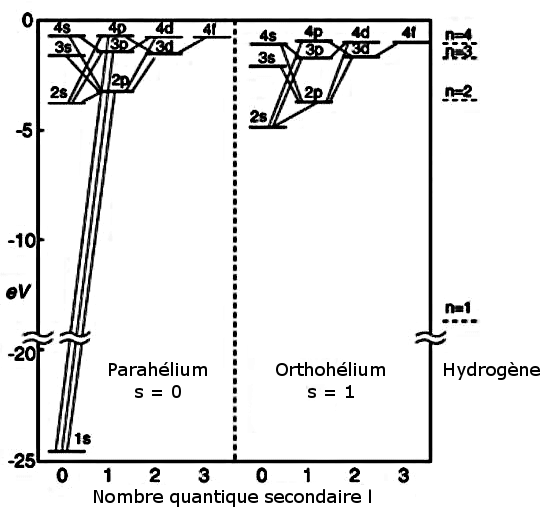
\includegraphics[scale=.7]{chimiePC/atomes/helium.png}
        \caption{Niveaux énergétiques de l'hélium comparés à ceux de l'hydrogène}
    \end{figure}
    
\end{EnvUplevel}
    \question Préciser ce que signifie $s= 0$ et $s = 1$.
    
    \question Représenter par deux diagrammes énergétiques la configuration électronique fondamentale du parahélium et de l'orthohélium. Pourquoi le l'orthohélium n'a pas de niveau 1s sur le schéma ? \'Enoncer la règle illustrée ici.
    \question Comparer les niveaux d'énergie 1s du parahélium et de l'hydrogène et expliquer cette différence.
    \question Représenter les niveaux énergétique des sous-couches de l'hydrogène pour $n\leqslant 3$.
    \question Comparer les les niveaux d'énergie des sous-couches de $n=2$ entre le parahélium et l'hydrogène. Comment s'appelle ce phénomène ?
    \questionbonus Pourquoi ce phénomène n'est pas présent dans l'hydrogène ?
    \question Commenter (sans expliquer) l'ordre des sous-couches $n=3$ et $n=4$ dans le parahélium. \'Enoncer la règle violée.
    \question Comment qualifier les niveaux énergétiques des orbitales atomiques au sein d'une même sous-couche ?
    \question Retrouver la formule donnant le nombre d'orbitales atomiques et le nombre maximal d'électrons dans une couche donnée.
    \question Comparer les les niveaux d'énergie des sous-couches de $n=2$ entre le parahélium et l'orthohélium. \'Enoncer la règle de remplissage illustrée ici ?
    
\end{questions}
\end{exercise}
% Niveau :      PCSI *
% Discipline :  Chimie Orga I
% Mots clés :   Spectrométrie UV-visible, Réactions acidobasiques

\begin{exercise}{Réactivité et électronégativité}{2}{PCSI}
{Atomistique,Classification périodique, Structure électronique}{bermu}

\begin{questions}
    \questioncours \'Evolution de l'énergie de liaison et de l'électronégativité des atomes dans la classification périodique. 
    On illustrera à l'aide de la figure ci-dessous.
    
\begin{EnvUplevel}
    \begin{figure}[H]
        \centering
        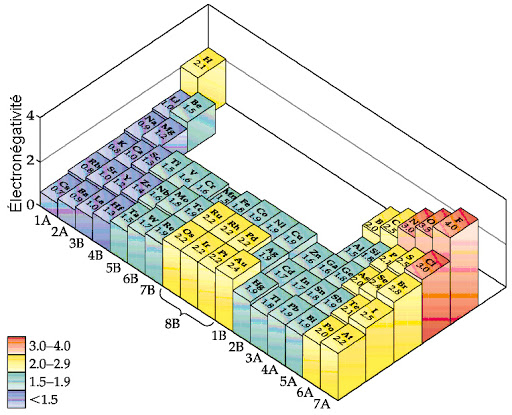
\includegraphics[scale=.6]{chimiePC/atomes/electroneg.jpg}
        \caption{\'Evolution de l'électronégativité au sens de Pauling dans la classification périodique.}
        \label{fig:my_label}
    \end{figure}
\end{EnvUplevel}

\begin{EnvUplevel}
On étudie la réactivité de différents composés organométalliques H$_3$C--M, où M est un atome métallique. Selon l'atome M, la réaction conduit à deux produits \textbf{A} et \textbf{B} en proportion variable comme l'indique la table ci-dessous.

\begin{table}[H]
    \centering
    \begin{tabular}{rlccr}
        Organométallique & H$_3$C--M  & \% ion. C--M & \textbf{A} : \textbf{B} \\ \hline\hline
        Organopotassique      & H$_3$C--K    & 53 & $\sim 1:0$~ \\
        Organosodique         & H$_3$C--Na   & 48 & $99:1$~ \\
        Organolithien         & H$_3$C--Li   & 46 & $98:2$~ \\
        Organomagnésien mixte & H$_3$C--MgBr & 32 & $86:14$ \\
        Organozincique mixte  & H$_3$C--ZnBr & 32 & $72:28$ \\
        Organocuprate lithié  & H$_3$C--CuLi & 10 & $\sim 0:1$~ \\ \hline
    \end{tabular}
    \caption{Propriétés et sélectivité de différents composés organométalliques.}
\end{table}
\end{EnvUplevel}

\question Que signifie l'appellation 'atome métallique' ? Cette appellation est-elle propre ? Décrire quels atomes de la classification périodique peuvent être qualifiés de métalliques.

\question Expliquer l'évolution du pourcentage d'ionicité de la liaison C--M dans la table ci-dessus.

\question Justifier que la réactivité de H$_3$C--M est conditionnée par l'ionicité de la liaison C--M. \\
Réécrire H$_3$C--M dans la limite d'un comportement 100 \% ionique.

\question Donner rapidement la configuration électronique de valence des atomes métalliques K, Na, Li, Mg, Zn, Cu et Mg. \\
On utilisera les abréviation [He], [Ar] et [Ne] (resp. 1$^\text{ère}$, 2$^\text{ème}$ et 3$^\text{ème}$ période).

\question À l'aide de la question précédente, justifier la forme des composés organométalliques (qui sont quasi-ioniques) dans la table ci-dessus.

\question Définir et décrire l'évolution du potentiel d'ionisation dans la table périodique.

\question Les organométalliques H$_3$C--M réagissent très bien avec H$_3$C--Br. Justifier susccintement.

\question Décrire et commenter succinctement l'évolution de la proportion \textbf{A} : \textbf{B}.

\question Qu'en-est-il du rayon ionique de M ?

\end{questions}

\end{exercise}
% Niveau :      PCSI *
% Discipline :  Chimie Orga I
% Mots clés :   Spectrométrie UV-visible, Réactions acidobasiques

\begin{exercise}{Magnétisme et table périodique}{3}{PCSI}
{Atomistique,Classification périodique, Structure électronique}{bermu}

\paragraph{Question ouverte :} après avoir rappelé ce qui caractérise la configuration électronique fondamentale des atomes diamagnétiques et paramagnétiques, décrire et justifier la table ci-dessous dans la mesure de vos connaissances.


    \begin{figure}[H]
        \centering
        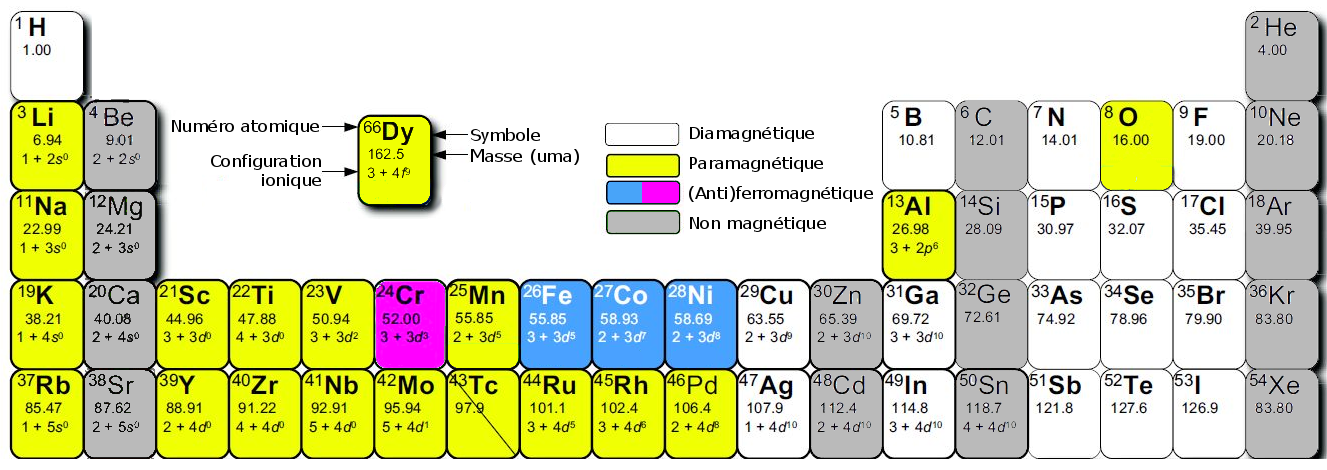
\includegraphics[width=\linewidth]{chimiePC/atomes/magnet.png}
        \caption{Propriétés magnétiques et tableau périodique}
    \end{figure}

\end{exercise}
% Niveau :      PCSI *
% Discipline :  Chimie Orga I
% Mots clés :   Spectrométrie UV-visible, Réactions acidobasiques

\begin{exercise}{Chimie click, chimie verte}{2}{PCSI}
{Solvants}{bermu}



\begin{questions}
    \questioncours Différentes étapes de la solvatation d'un soluté dans un solvant. \\
    On illustrera la question d'exemple en rentrant dans le détail des différents types de solvants.

\begin{EnvUplevel}
Un des principes très importants de chimique organique est de réduire la quantité de solvants organiques utilisés.

Une des tendances actuelles en chimie de synthèse est la chimie click au micro-onde de la réaction de Biginelli :
\begin{center}
    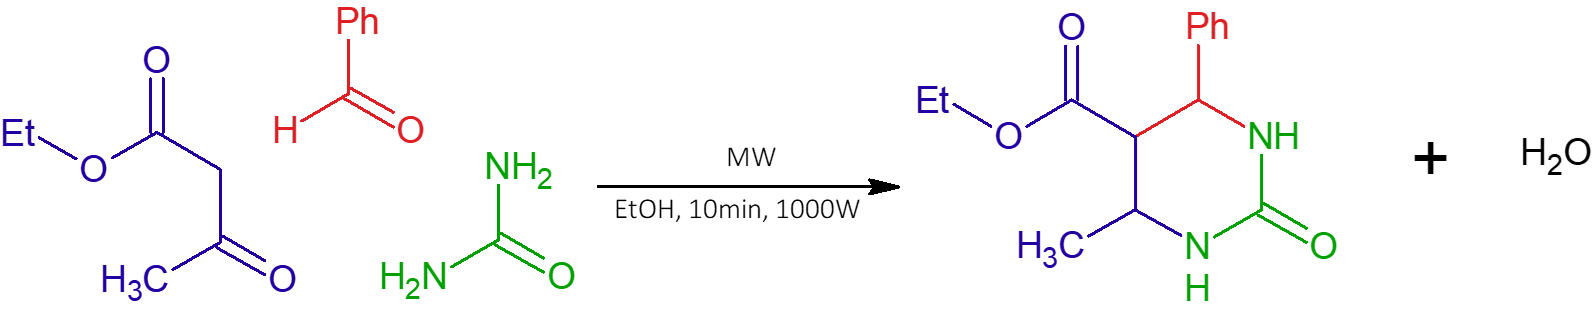
\includegraphics[width=.9\linewidth]{chimiePC/atomes/click.png}
\end{center}

\end{EnvUplevel}
    
    \question Classiquement, pour faire une telle réaction on utilise du toluène et un catalyseur qui sont tous deux très polluants.
    
    \begin{parts}
        \part Justifier le choix du toluène (solvant apolaire).
        
        \part \`A la suite de la réaction, il faut ensuite extraire le produit. Donner le principe de l'extraction par solvants et indiquer ici un solvant que l'on pourrait utiliser pour cela.
    
    \end{parts}
    
    \question En chimie click, on utilise uniquement de l'éthanol pour la réaction. Celle-ci est activée grace aux micro-ondes.
    
    \begin{parts}
        \part Justifier le choix de l'éthanol.
        
        \part Justifier que l'éthanol est excité par les micro-ondes et que cela permet de catalyser la réaction.
    \end{parts}
    
    \question Conclure quant aux gains écologique pour réaliser cette réaction. Pour information les 12 principes de la chimie verte ci-dessous.
    
    \begin{table}[H]
        \centering
        \begin{tabular}{ll}
            \\\hline\hline
            1. Prévention : moins de déchets ; &
            7. Matières renouvelables  ;\\
            2. Économie d'atomes : moins de sous-produits ; &
            8. Schéma de synthèse efficace ;\\
            3. Réactif doux : pas de substances toxiques ; &
            9. Catalyse ;\\
            4. Réduire la toxicité des produits utilisés ; &
            10. Produits biodégradables ;\\
            5. Pas de substances auxiliaires (solvants...) &
            11. Contrôle des conditions de réaction ; \\
            6. Conditions douces : CNTP ; &
            12. Réduire les risques d'accidents. \\ \hline
        \end{tabular}
        \caption{Principes de la chimie verte}
    \end{table}
    
    \question (\emph{Bilan}) Récapituler les rôles du solvant en chimie de synthèse et la manière de réduire son impact écologique.
\end{questions}
\end{exercise}

\section{Stéréochimie}
% Niveau :      PCSI *
% Discipline :  Chimie Orga
% Mots clés :   Stéréochimie

\begin{exercise}{Benzène de Ladenburg}{2}{PCSI}
{Chimie organique I,Stéréochimie}{jbb}

\begin{questions}
\questioncours Répondre aux questions suivantes en redéfinissant les notions abordées et en les illustrant par un (des) exemple(s) pertinent(s).
\hspace*{-1ex}\begin{tabbing}
    \textsf{\bfseries a) } Une molécule qui possède (ne possède pas) un axe de symétrie \hspace{3ex} \= est-elle (a)chirale ? \\
    \textsf{\bfseries b) } Une molécule qui possède (ne possède pas) un plan de symétrie \> est-elle (a)chirale ? \\
    \textsf{\bfseries c) } Une molécule qui possède (ne possède pas) un centre de symétrie \> est-elle (a)chirale ? \\
    \textsf{\bfseries d) } Quel est le lien entre les stéréodescripteurs L,D et R,S ?
\end{tabbing}


\begin{EnvUplevel}
    Au XIX\textsuperscript{ème} siècle, la structure du benzène était un mystère pour les chimistes. Seule la formule brute $\mathrm{C_6H_6}$ était connue. En 1874, Ladenburg a proposé de présenter la structure du benzène sous forme d'un prisme droit à base triangulaire dont chaque sommet était un atome de carbone lié à un atome d'hydrogène.
\end{EnvUplevel}

\question Représenter le benzène de Ladenburg sous forme semi-développée.

\question Les benzènes disubstitués $\mathrm{C_6H_4X_2}$, pour lequel on a remplacé deux liasons C--H par une liaison C--X, existent sous forme de trois isomères isolés expérimentalement.
\begin{parts}
    \part Montrer que la structure proposée est compatible avec ce fait et donner les isomères en question.
    \part Comment peut-on isoler expérimentalement ces isomères ?
\end{parts}

\question En 1876, Van't Hoff a critiqué la structure de Ladenburg en indiquant qu'elle implique la présence d'énantiomères, ce qui est en contradiction avec les observations expérimentales effectuées jusqu'alors.
\begin{parts}
    \part Montrer que pour la structure proposée, les isomères du benzène disubstitué $\mathrm{C_6H_4X_2}$ donnent lieu à la formation d'énantiomères.
    \part Combien y a-t-il d'isomères (au sens large) au total ? \part Pourquoi certains isomères ne donnent pas lieu à des énantiomères ?
    \part Comment peut-on expérimentalement séparer ces isomères ?
    \part Conclure quant à l'objection de Van't Hoff.
\end{parts}

\question Reprendre la question précédente avec un benzène disubstitué de deux groupes différents, \\
X et Y : $\mathrm{C_6H_4XY}$.

\question Rappeler la vraie structure du benzène (formule de Kékulé) et vérifier pour cette formule que toutes les observations expérimentales sont compatibles.
\paragraph{Rappel :} le benzène est un cyclohexane dont les liaisons sont par alternance simples et doubles.

\end{questions}

\plusloin Pouvez-vous penser à d'autres structures que celles de Kékulé et Ladenbourg ?

\end{exercise}

\section{Polarimétrie}
% Niveau :      PCSI *
% Discipline :  Chimie Orgam
% Mots clés :   Ballistique, Mécanique du point, PFD, Chute libre

\begin{exercise}{Excès énantiomérique}{1}{PCSI}
{Chimie organique I,Polarimétrie,Excès énantiomérique,Pouvoir optique}{poublanc}
\index{\'Enantiomère}

\begin{questions}
\questioncours Loi de Biot. On fera bien attention de préciser les dépendances implicites des paramètres et les hypothèses de validité de la loi.

\begin{EnvUplevel}
    L'époxydation de Sharpless (prix Nobel de chimie 2001) permet la formation d'époxydes à partir d'alcools allyliques, selon le schéma réactionnel :
    
    Dans cette réaction l'excès énantiométrique est $\mathrm{e.e.} = 94 \%$.
    
    \paragraph{Rappel :}en notant $[\textsfbf{R}]$ et $[\textsfbf{S}]$ les concentrations respectives des énantiomères R et S, on définit l'excès énantiomérique comme
    $$\mathrm{e.e.} = \abs{\dfrac{[\textsfbf{R}] - [\textsfbf{S}]}{[\textsfbf{R}] + [\textsfbf{S}]}}.$$
\end{EnvUplevel}

\question Entre quelles bornes l'excès énantiométrique $\mathrm{e.e.}$ peut varier ? Dans quelles cas les bornes sont atteintes ?
\question Déterminer les pourcentages des composés \textsfbf{R} et \textsfbf{S} dans le mélange de produits ? Commenter.

\begin{EnvUplevel}
    Afin de mesurer l'excès énantiométrique et donc la stéréosélectivité de la aréaction, on utilise la polarimétrie. En notant $\alpha_\text{max} >0$ la valeur absolue du pouvoir rotatoire d'une solution énantiomériquement pure à la concentration $C_1$, on définit le pouvoir optique $\mathrm{p.o.}$ comme le rapport
    $$\mathrm{p.o.} = \abs{\dfrac{\alpha}{\alpha_\text{max}}}.$$
\end{EnvUplevel}

\question Etablir la relation entre l'excès énantiométrique $\mathrm{e.e.}$ et le pouvoir optique $\mathrm{p.o.}$ Quel est le pouvoir optique de cette solution ?


\question Sous quelles conditions la donnée expérimentale du pouvoir optique p.o. permet-elle de remonter à l'excès énantiomérique. On prendra gare au fait que les angles sont définis à $2\pi$ près.

\question Comment généraliser ces résultats avec des diastéréoisomères ?

\end{questions}
\end{exercise}

\section{Spectrométrie UV-visible}
% Niveau :      PCSI *
% Discipline :  Chimie Orga
% Mots clés :   Infrarouge

\begin{exercise}{Spectroscopies d'absorption}{0}{PCSI}
{Chimie organique I,Spectroscopie}{bermu}

\begin{questions}
\question Rappelez brièvement le principe physique des spectroscopies d'absorption et d'émission.

\uplevel{Par la suite, nous allons évoquer différents types de spectroscopies. On les placera sur un diagramme ayant pour axe la fréquence / la longueur d'onde / l'énergie des transitions employées.}

\question On considère tout d'abord une molécule monoatomique (\emph{e.g.} He).
\begin{parts}
    \part Quelles transitions énergétiques y a-t-il pour une telle molécule ?
    \part Placer sur le diagramme l'ordre de grandeur des fréquences en jeu.
    \part Quelle loi connaissez-vous concernant les niveaux d'énergie de ces transitions ?
    \part Donnez un ou des exemple$\cdot$s de spectroscopie$\cdot$s mettant en jeu ces transitions.
    \part Quel$\cdot$s objet$\cdot$s du quotidien met$\cdot$tent en jeu de telles transitions ?
\end{parts}
\question On considère à présent une molécule polyatomique (\emph{e.g.} $\mathrm{NO_2}$). Quels nouveaux types de transitions faut-il considérer ? Reprendre les étapes de la question précédente pour chaque type de transition.

\end{questions}

\end{exercise}
% Niveau :      PCSI *
% Discipline :  Chimie Orga I
% Mots clés :   Spectrométrie UV-visible, Réactions acidobasiques

\begin{exercise}{Bleu de bromothymol}{2}{PCSI}
{Chimie organique I,Spectroscopie,UV-visible,Réactions acidobasiques}{bermu}

\begin{questions}
\questioncours Loi de Beer-Lambert. On fera bien attention de préciser les dépendances implicites des paramètres et les hypothèses de validité de la loi.

\begin{EnvUplevel}
    Le bleu de bromothymol (BBT) est un indicateur de pH très utilisé en biologie pour mettre en présence le $\mathrm{CO_2}$. Vers $\text{pH} = 7.0$, il passe de sa forme acide jaune à sa forme basique bleue (notées $\mathrm{InH}$ et $\mathrm{In^{-}}$) :\vspace{-1em}
    \begin{figure}[H]
        \centering
        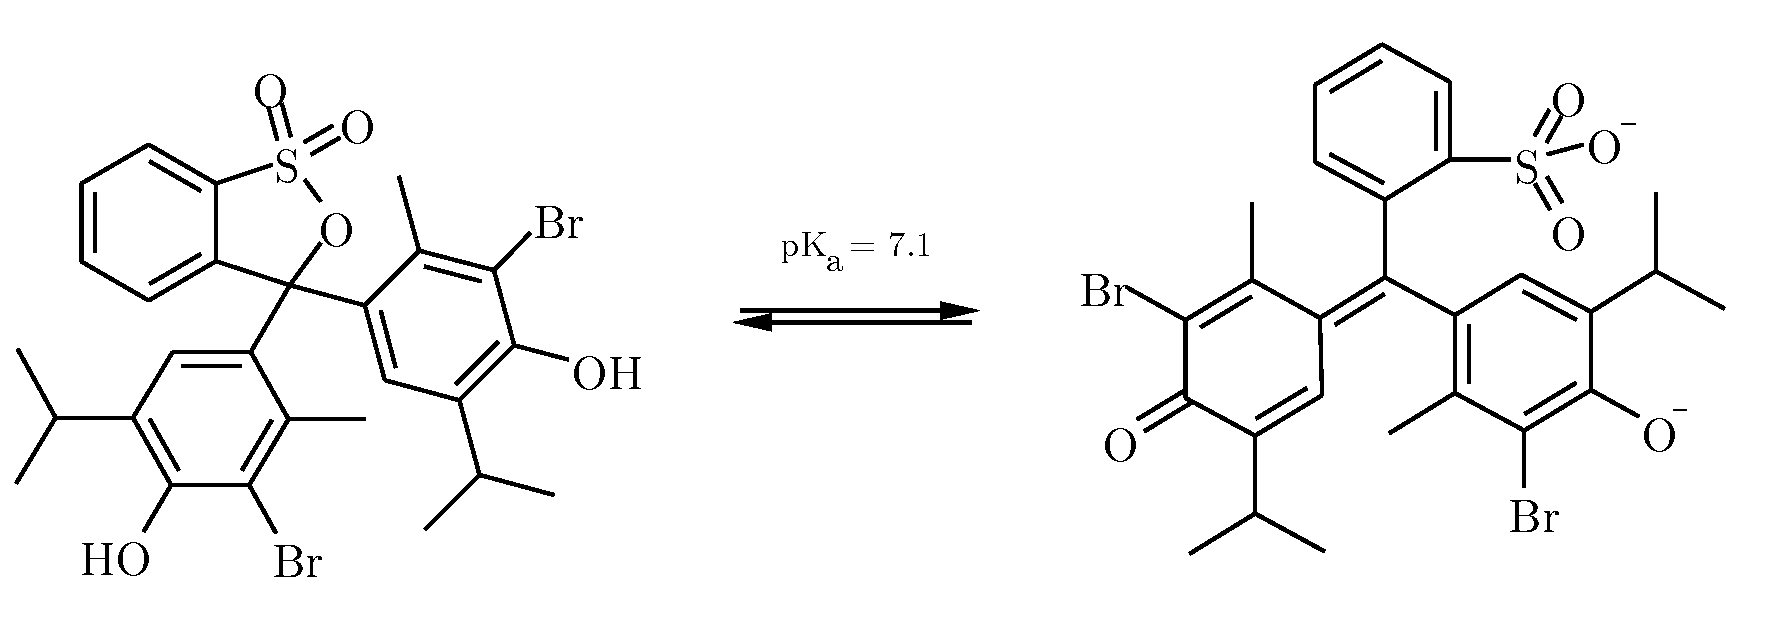
\includegraphics[width=.6\linewidth]{chimiePC/orga/BBT1.pdf}\vspace{-2em}
        \caption{\'Equilibre acidobasique du bleu de bromothymol.}
        \label{fig:BBT1}\vspace{-1em}
    \end{figure}
    
    Dans une publication récente (Hui Hou, \emph{Nature Scientific Reports}, 7:1759, 2017), les auteurs proposent une méthodologie pour mesurer le pH par mesure de l'absorbance.
    \begin{figure}[H]
        \centering
        \begin{tabularx}{\linewidth}{XX}
            \small{\textbf{(a)}} & \small{\textbf{(b)}}. \\
            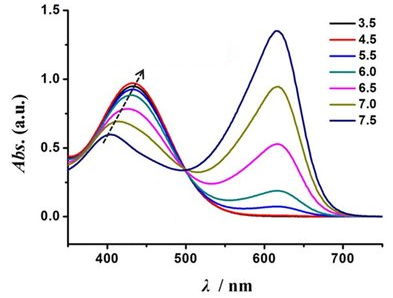
\includegraphics[width=\linewidth]{chimiePC/orga/BBT2.png} &
            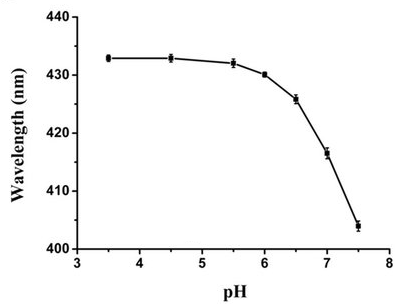
\includegraphics[width=\linewidth]{chimiePC/orga/BBT3.png}
        \end{tabularx}\vspace{-1em}
        \caption{Spectres d'absorption UV-Visible (\textbf{a}) et courbe de calibration du pic à $\sim$ 420 nm (\textbf{b}) du bleu de bromothymol pour différentes valeurs de pH.}
        \label{fig:BBT2}
    \end{figure}
\end{EnvUplevel}\vspace{-1em}

\question Interpréter qualitativement la fig. \ref{fig:BBT2}a avec les deux maxima $\lambda_\text{max,a} = 433$ nm et {$\lambda_\text{max,b} = 616$~nm}.

\question\label{qu:1} Rappeler l'intérêt de mesurer l'absorbance au niveau des maxima d'intensité et justifier que
$$A(\lambda) \simeq A_\text{max} + \dfrac{1}{2}\dv[2]{A}{\lambda} \qty(\lambda - \lambda_\text{max})^2 \qqtext{pour} \lambda \simeq \lambda_\text{max}.$$

\question Le point $\lambda_i = 500$ nm est nommé un point isobestique. Justifier par un simple calcul que ce point d'absorption constante $A_i$ durant la transformation $\mathrm{InH \xrightleftharpoons{} In^- + H^+}$ indique que cette transformation ne fait pas intervenir d'intermédiaire. \vspace{-2em}
\begin{EnvUplevel}
\paragraph{Indication :} exprimer l'absorbance de la solution en fonction des concentrations $[\mathrm{In^-}]$ et $[\mathrm{InH}]$.

On va maintenant s'intéresser à modéliser la courbe de calibration.
\end{EnvUplevel}

\question La forme basique du BBT possède également un maximum d'absorption en $\lambda_\text{max,b'} = 403$~nm. A l'aide de l'approximation de la question \ref{qu:1}, modéliser la longueur d'onde maximale $\lambda_\text{max}$ en fonction des concentrations $[\mathrm{In^-}]$ et $[\mathrm{InH}]$.
\end{questions}

\plusloin
\`A l'aide de la relation d'Henderson--Hasselbalch et du $\mathrm{pK_a}$ du BBT, exprimer la relation $\lambda(\text{pH})$. 
\end{exercise}

\section{Spectroscopie IR}
% Niveau :      PCSI *
% Discipline :  Chimie Orga
% Mots clés :   IR

\begin{exercise}{Spectre infrarouge du nitrophénol}{1}{PCSI}
{Chimie organique I,Spectroscopie,Infrarouge}{bermu}

\begin{questions}
    \question Donnez la structure de l'ortho-nitrophénol, du méta-nitrophénol et du para-nitrophénol.
    \uplevel{\paragraph{Aide :}ortho, méta et para correspondent respectivement aux positions 2, 3 et 4 sur le cycle benzénique.}

    \question Sont donnés ci-dessous les spectres IR de ces trois espèces en phase gaz. Interprétez les différences observées.
    
    \uplevel{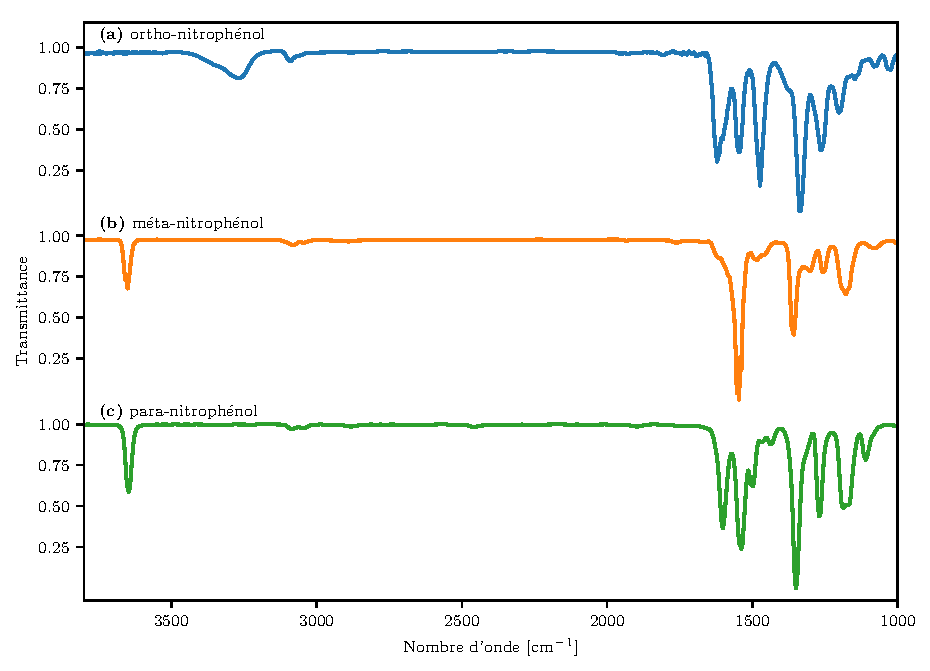
\includegraphics[width=\linewidth]{chimiePC/orga/nitro.pdf}}
    
    \question Qu'attendrait-on si les spectres étaient effectués en phase liquide ?
\end{questions}
\end{exercise}
% Niveau :      PCSI *
% Discipline :  Chimie Orga
% Mots clés :   Infrarouge

\begin{exercise}{Spectre infrarouge de l'eau}{2}{PCSI}
{Chimie organique I,Spectroscopie,Infrarouge}{bermu}

\begin{questions}
\questioncours Spectroscopie infrarouge
\begin{itemize}
    \item principe physique ;
    \item exemple d'une molécule diatomique simple ;
    \item paramètres influençant la fréquence de résonance et la largeur spectrale des raies ;
\end{itemize}

\uplevel{On considère désormais la molécule d'eau $\mathrm{H_2O}$.}

\question Donnez sa géométrie selon la théorie VSEPR.

\question Quels sont les différents modes de vibration de la molécule d'eau ? Les illustrer par un schéma.

\begin{EnvUplevel}
    On donne ci-dessous les spectres IR de l'eau $\mathrm{H_2O}$ et de l'eau ‘lourde’ $\mathrm{D_2O}$.
    
    \begin{figure}[H]
        \centering
        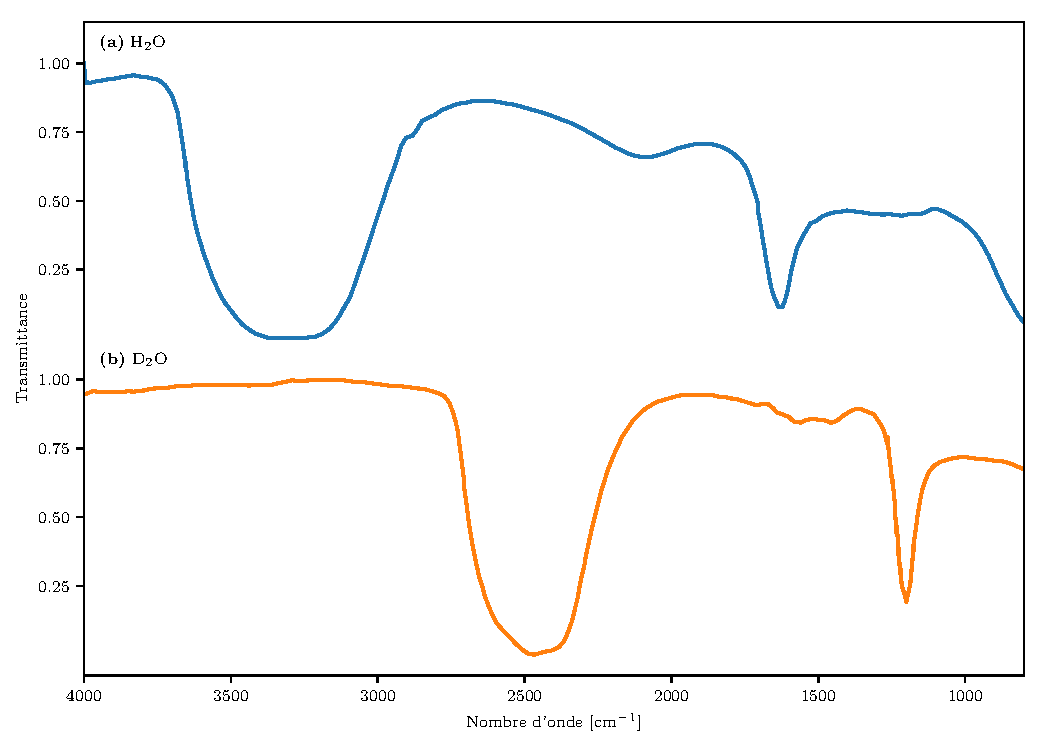
\includegraphics[width=\linewidth]{chimiePC/orga/H2OD2O.pdf}\vspace{-1em}
        \caption{Spectres infrarouges de l'eau et de l'eau lourde.}
    \end{figure}
\end{EnvUplevel}

\question Interprétez quantitativement les spectres ci-dessous à l'aide de la question de cours.

\question A quoi est dû le fort élargissement de la bande 3500 cm$^{-1}$ (2500 cm$^{-1}$ pour $\mathrm{D_2O}$) ?
\end{questions}
\end{exercise}
% Niveau :      PCSI *
% Discipline :  Chimie Orga
% Mots clés :   IR

\begin{exercise}{Spectre infrarouge des cétones cycliques}{3}{PCSI}
{Chimie organique I,Spectroscopie,Infrarouge}{bermu}

\begin{questions}
    \questioncours Spectroscopie infrarouge.
\begin{itemize}
    \item allure d'un spectre IR ;
    \item mesure d'un spectre IR ;
    \item fonctionnement de l'appareil (grandes lignes) ;
    \item paramètres influençant la vibration d'une liason donnée (\emph{e.g.} C=O) ;
\end{itemize}
    \question Interprétez les différences observées dans les spectres des différentes cétones ci-dessous :
\end{questions}
\noindent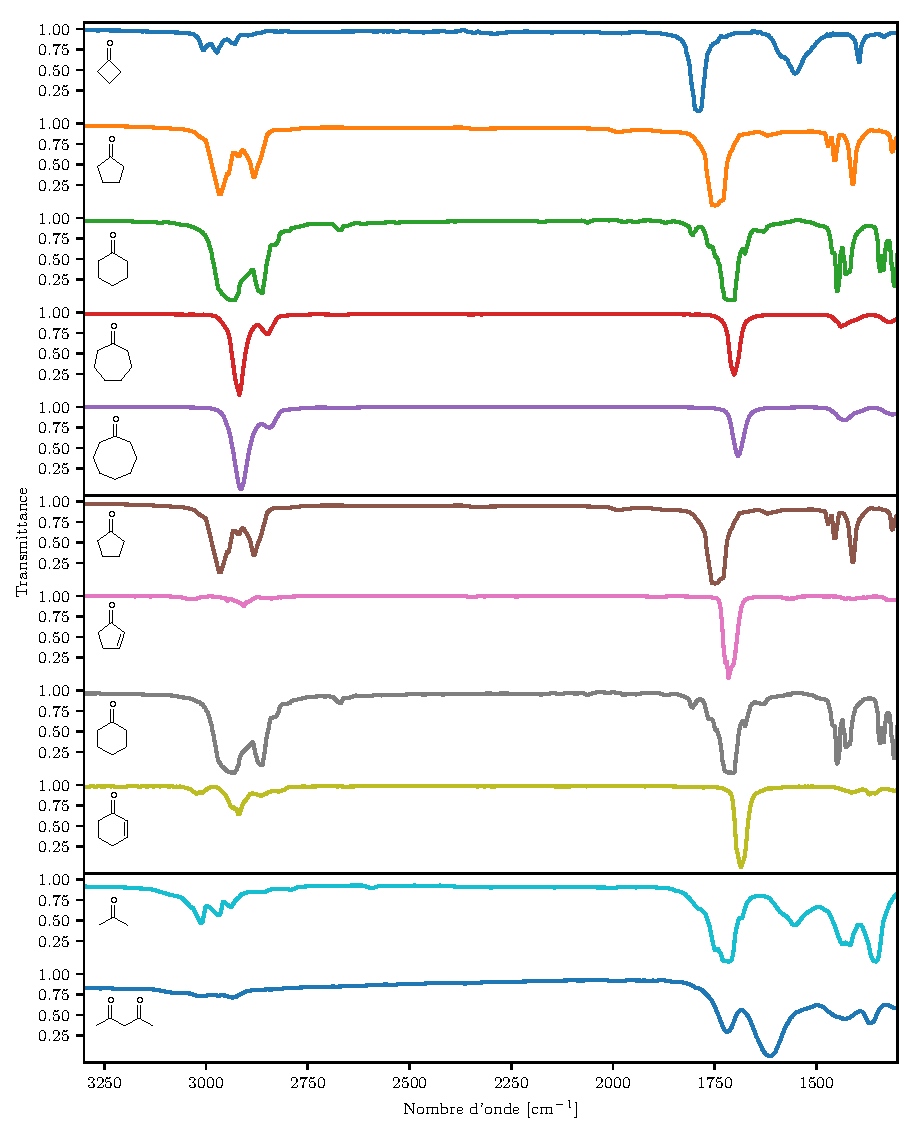
\includegraphics[width=\linewidth]{chimiePC/orga/cetones_ir_fig.pdf}
\end{exercise}

\section{RMN}
% Niveau :      PCSI *
% Discipline :  Chimie Orga
% Mots clés :   Stéréochimie

\begin{exercise}{Couplage \textit{J} dans les diènes}{3}{PCSI}
{Chimie organique I,Spectroscopie,RMN,Stéréochimie}{bermu}

\begin{questions}
\questioncours Couplage spin-spin $^{2}J$, $^{3}J$ et $^{4}J$ en RMN du proton $^{1}$H. \\
On prendra soin d'expliquer l'origine du phénomène sur un exemple simple et d'énoncer des facteurs d'influence de la valeur de $J$.

\begin{EnvUplevel}
On s'intéresse par la suite au couplage spin-spin dans les diènes conjugués à 6 carbones $\mathrm{C_6H_{10}}$

\begin{center}
    \chemfig{X-[1](-[3]X)=[-1](-[-3]X)-[1](-[3]X)=[-1](-[-3]X)-[1]X},
\end{center}
où X désigne un hydrogène ou groupe méthyle.

Les spectres RMN de ces espèces sont donnés dans l'annexe ci après.
\end{EnvUplevel}

\question Lister les isomères \underline{de constitution} de la forme donnée et donner leur nomenclature IUPAC.

\question Pour chaque isomère, établir quels spectres RMN peuvent (ou non) lui correspondre.

\question Parmi ces isomères, combien donnent lieu à des stéréoisomères \underline{de configuration} ? \\
Lister les différents stéréodescripteurs possibles pour chaque isomère de constitution.

\uplevel{Pour attribuer à chaque stéréoisomère un spectre, nous allons nous intéresser aux couplages $J$.}

\question Retrouver dans la mesure du possible les couplages $J$ du signal ddd dans le spectre \textbf{(\textit{a})}. \\
Pourquoi on ne peut pas retrouver tous les couplages ?

\question Essayez dans la mesure du possible d'attribuer pour chaque stéréodescripteur le spectre qui lui est associé. On pourra s'aider de l'annexe du handbook.
\end{questions}

\end{exercise}

\cleardoublepage

\subsection*{Annexe : spectres RMN $^{1}$H des diènes}

\begin{center}
    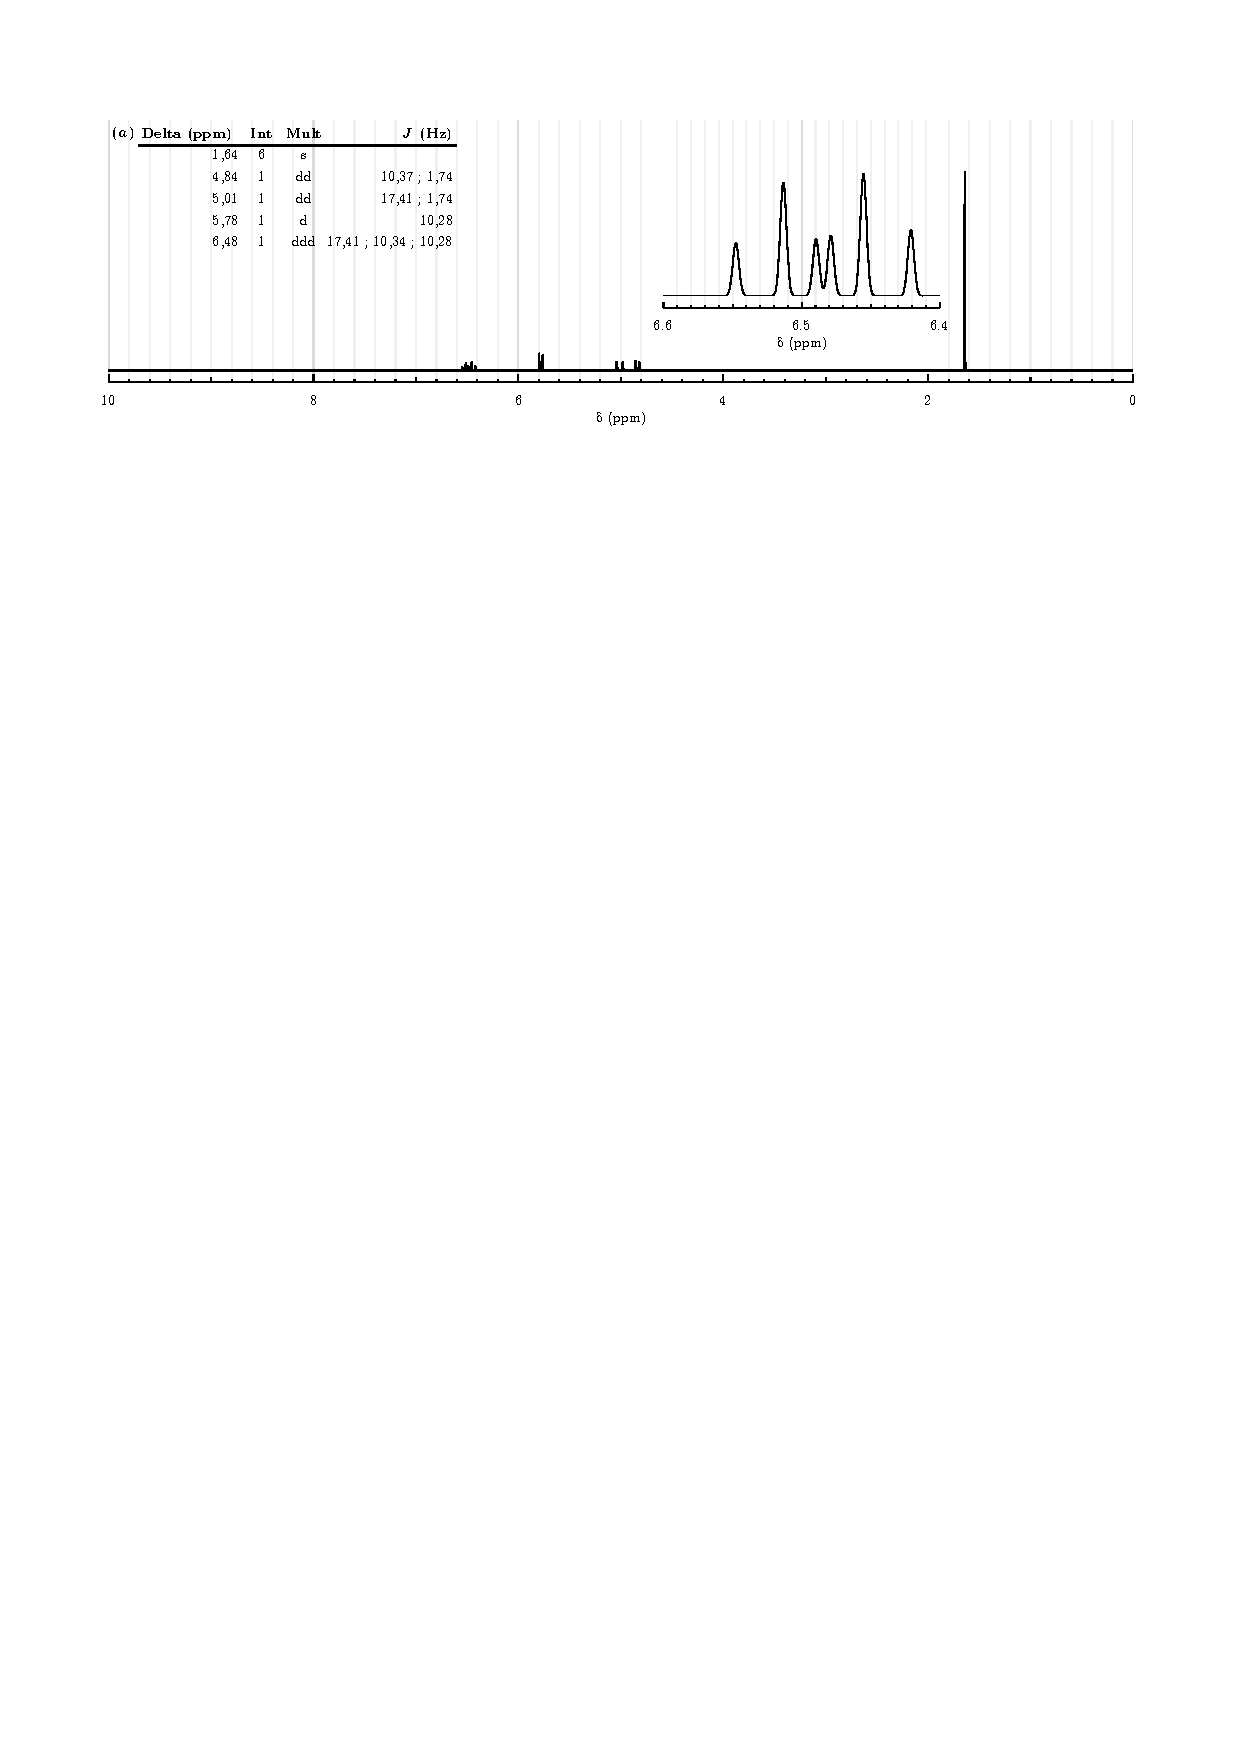
\includegraphics[width=.95\linewidth]{chimiePC/orga/RMN_4met.pdf}
    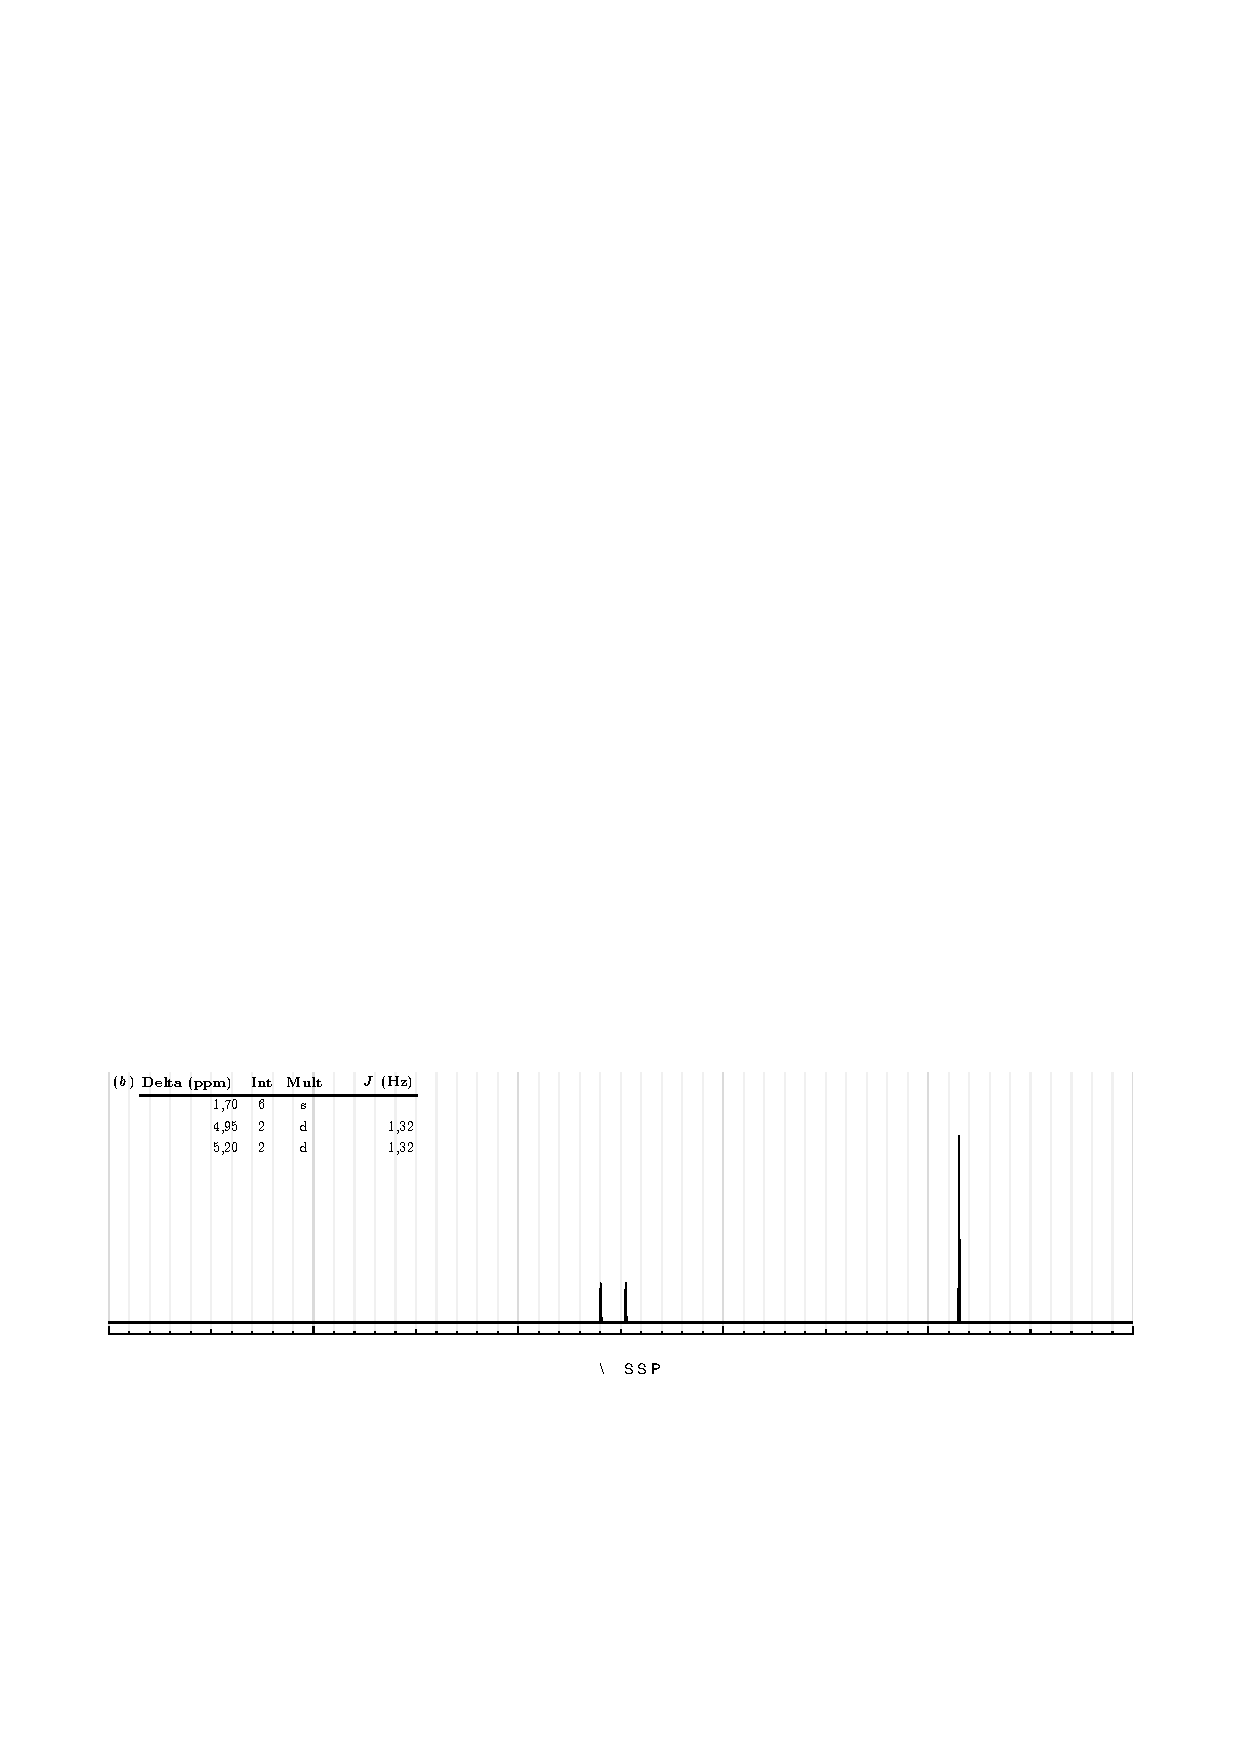
\includegraphics[width=.95\linewidth]{chimiePC/orga/RMN_23.pdf}
    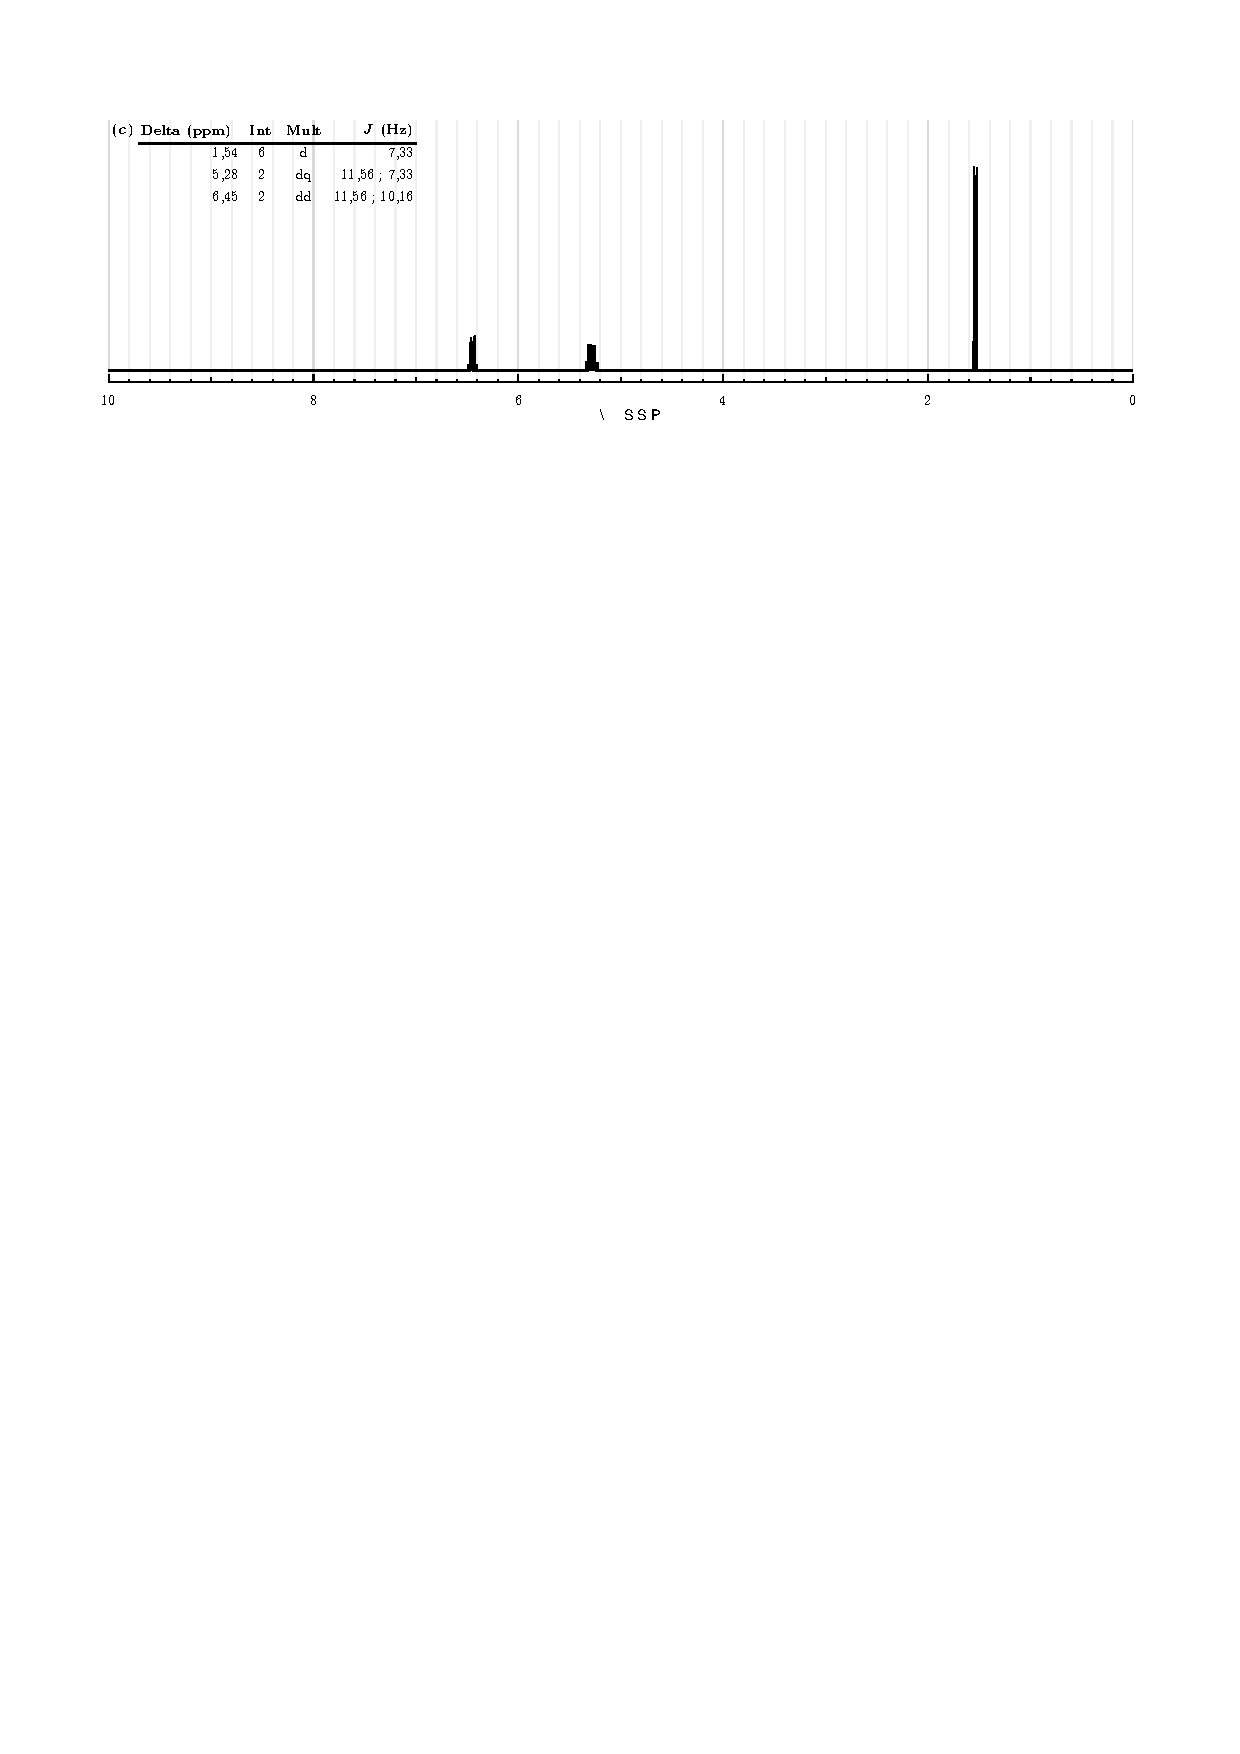
\includegraphics[width=.95\linewidth]{chimiePC/orga/RMN_ZZ.pdf}
    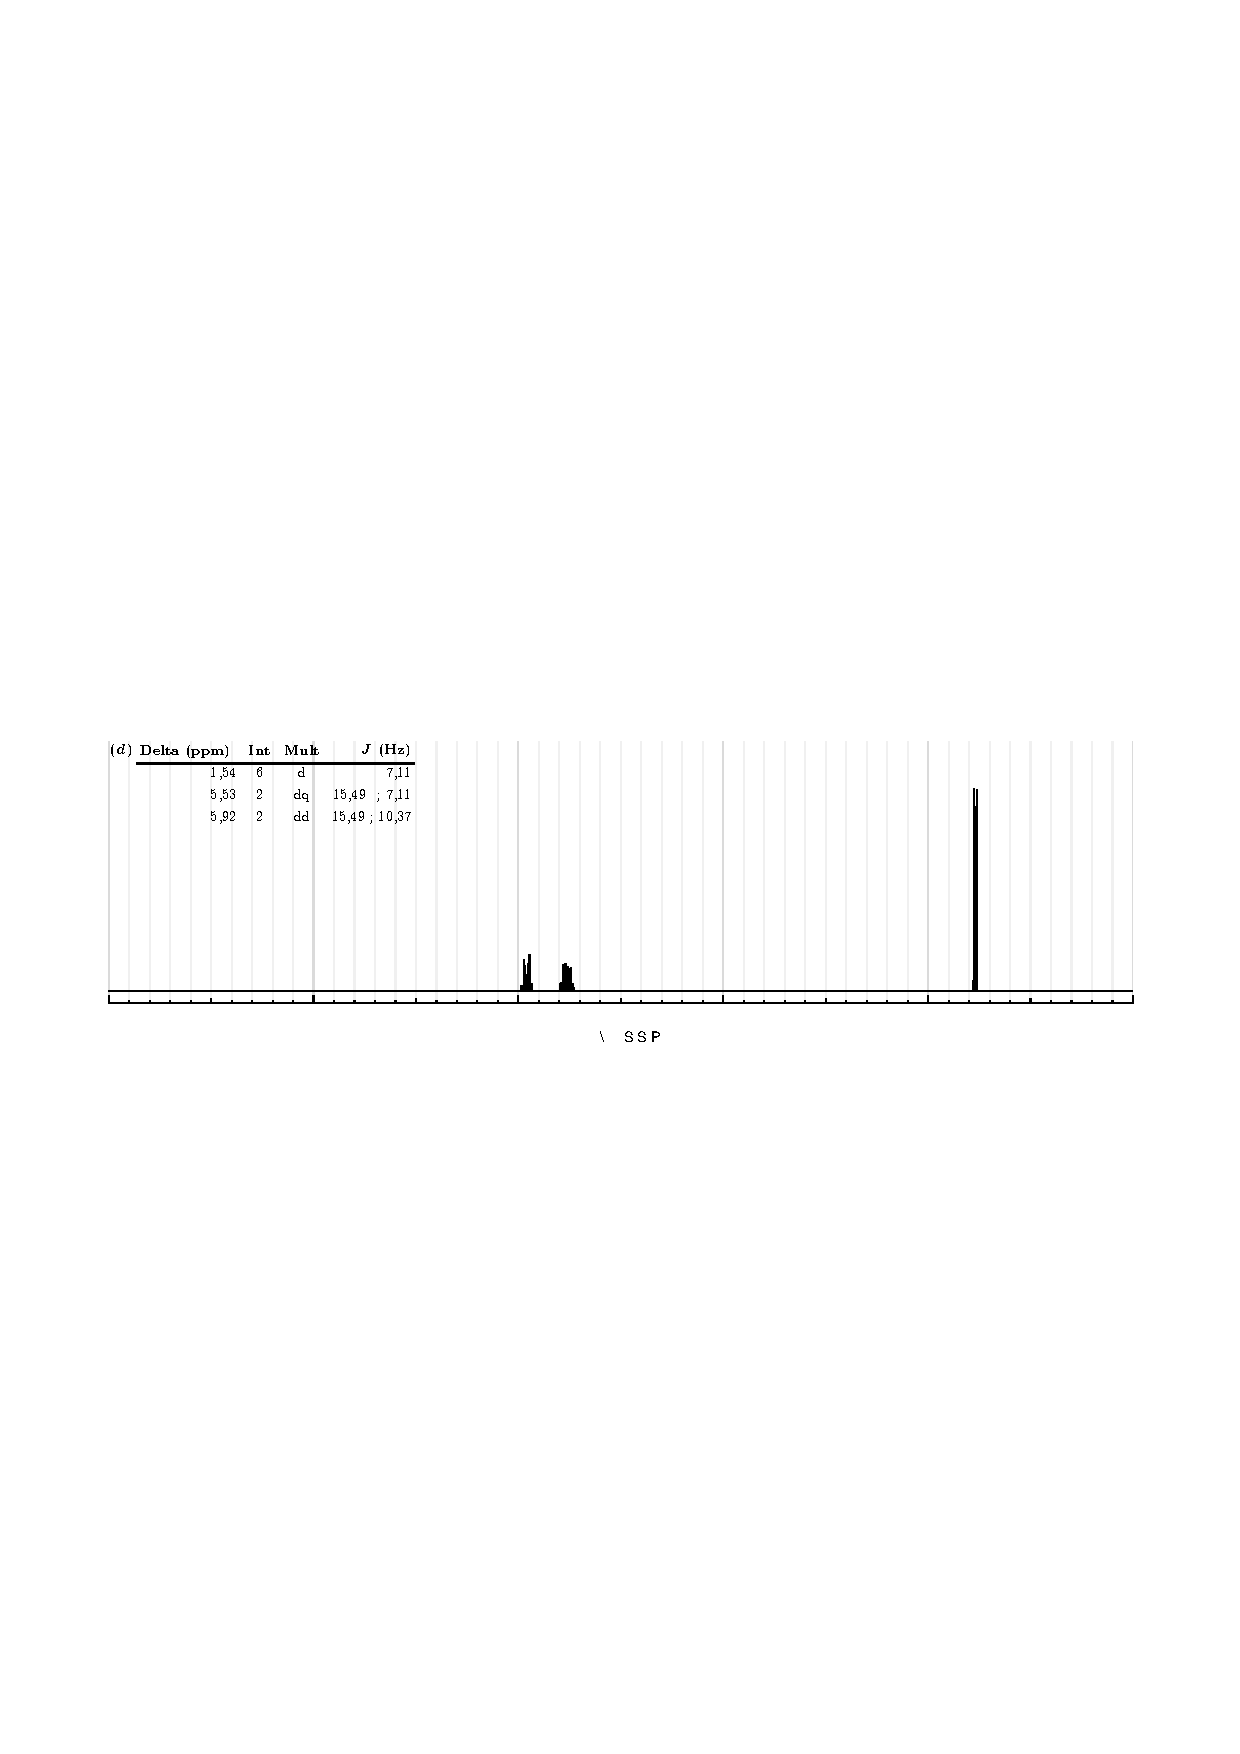
\includegraphics[width=.95\linewidth]{chimiePC/orga/RMN_EE.pdf}
    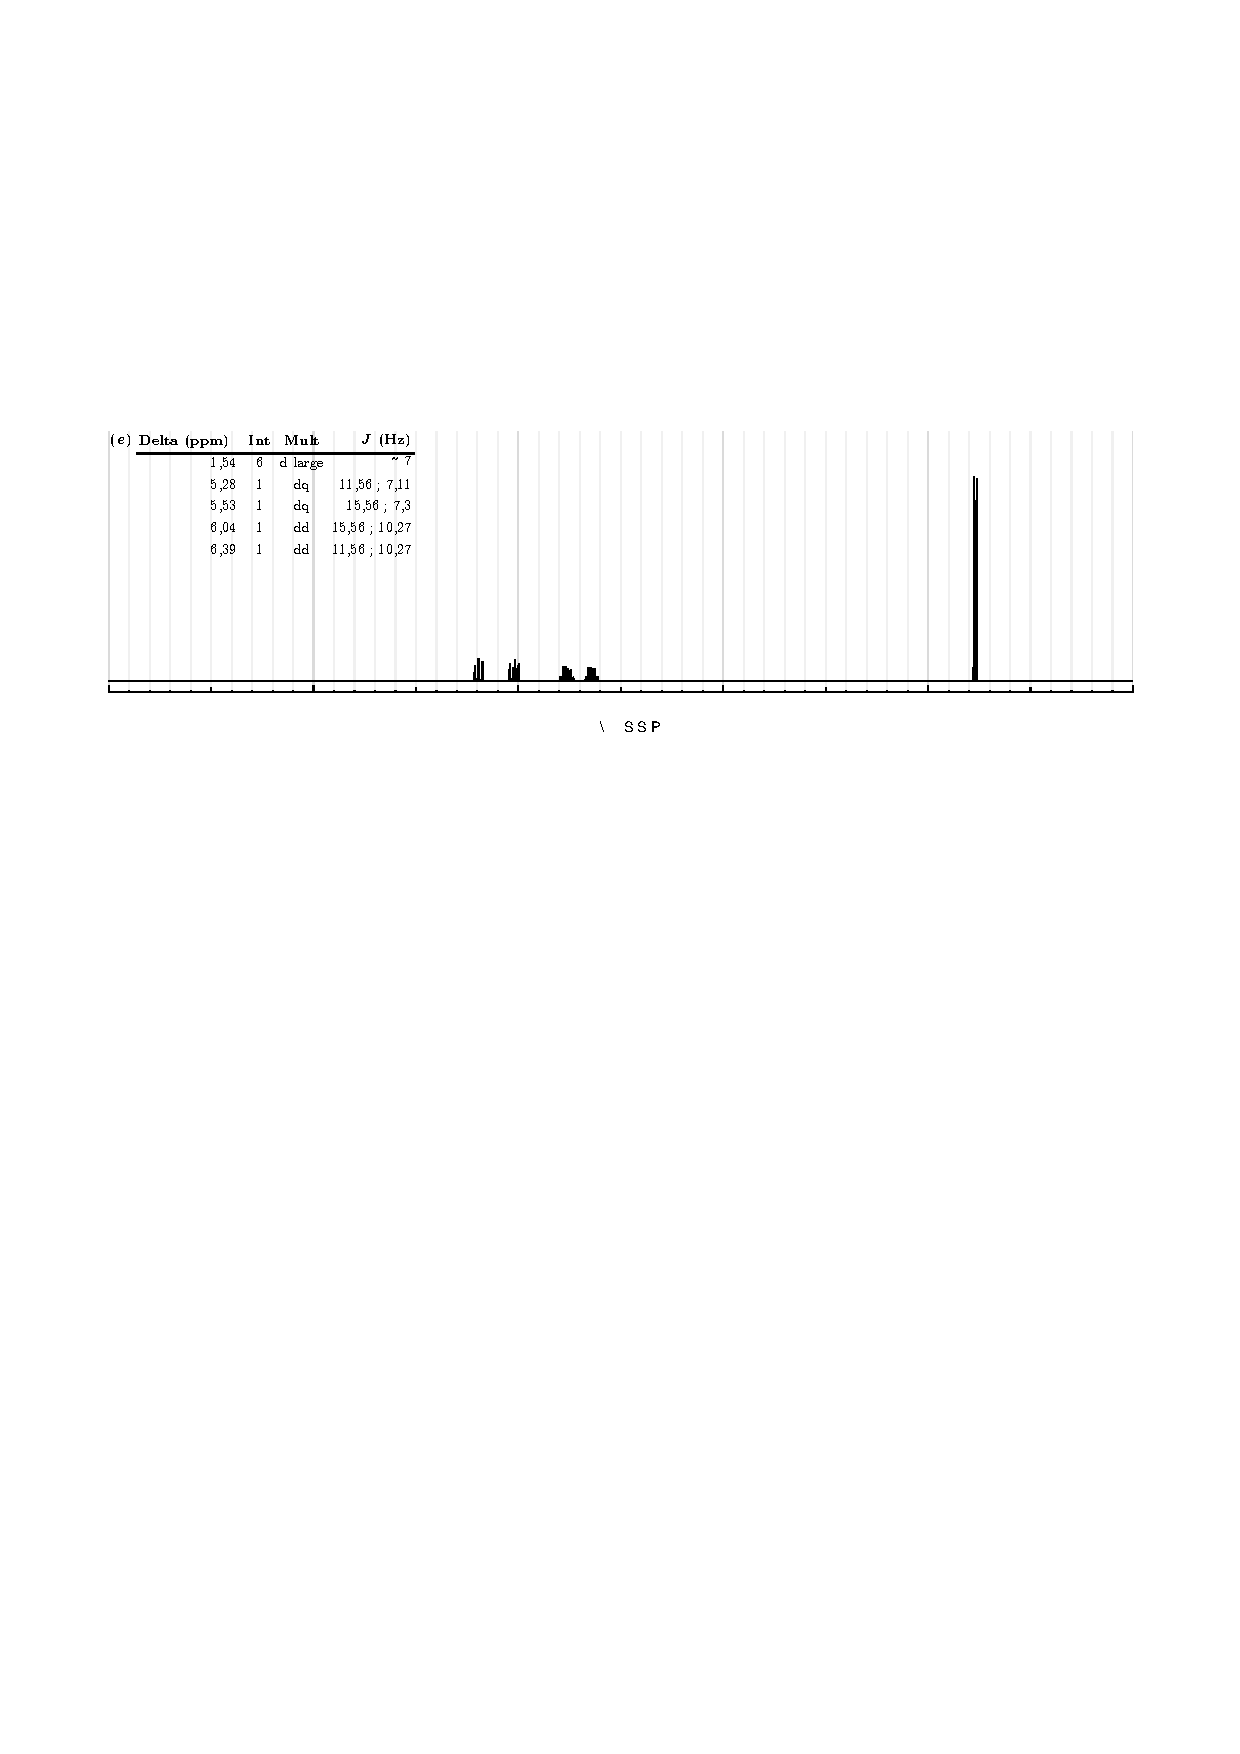
\includegraphics[width=.95\linewidth]{chimiePC/orga/RMN_ZE.pdf}
    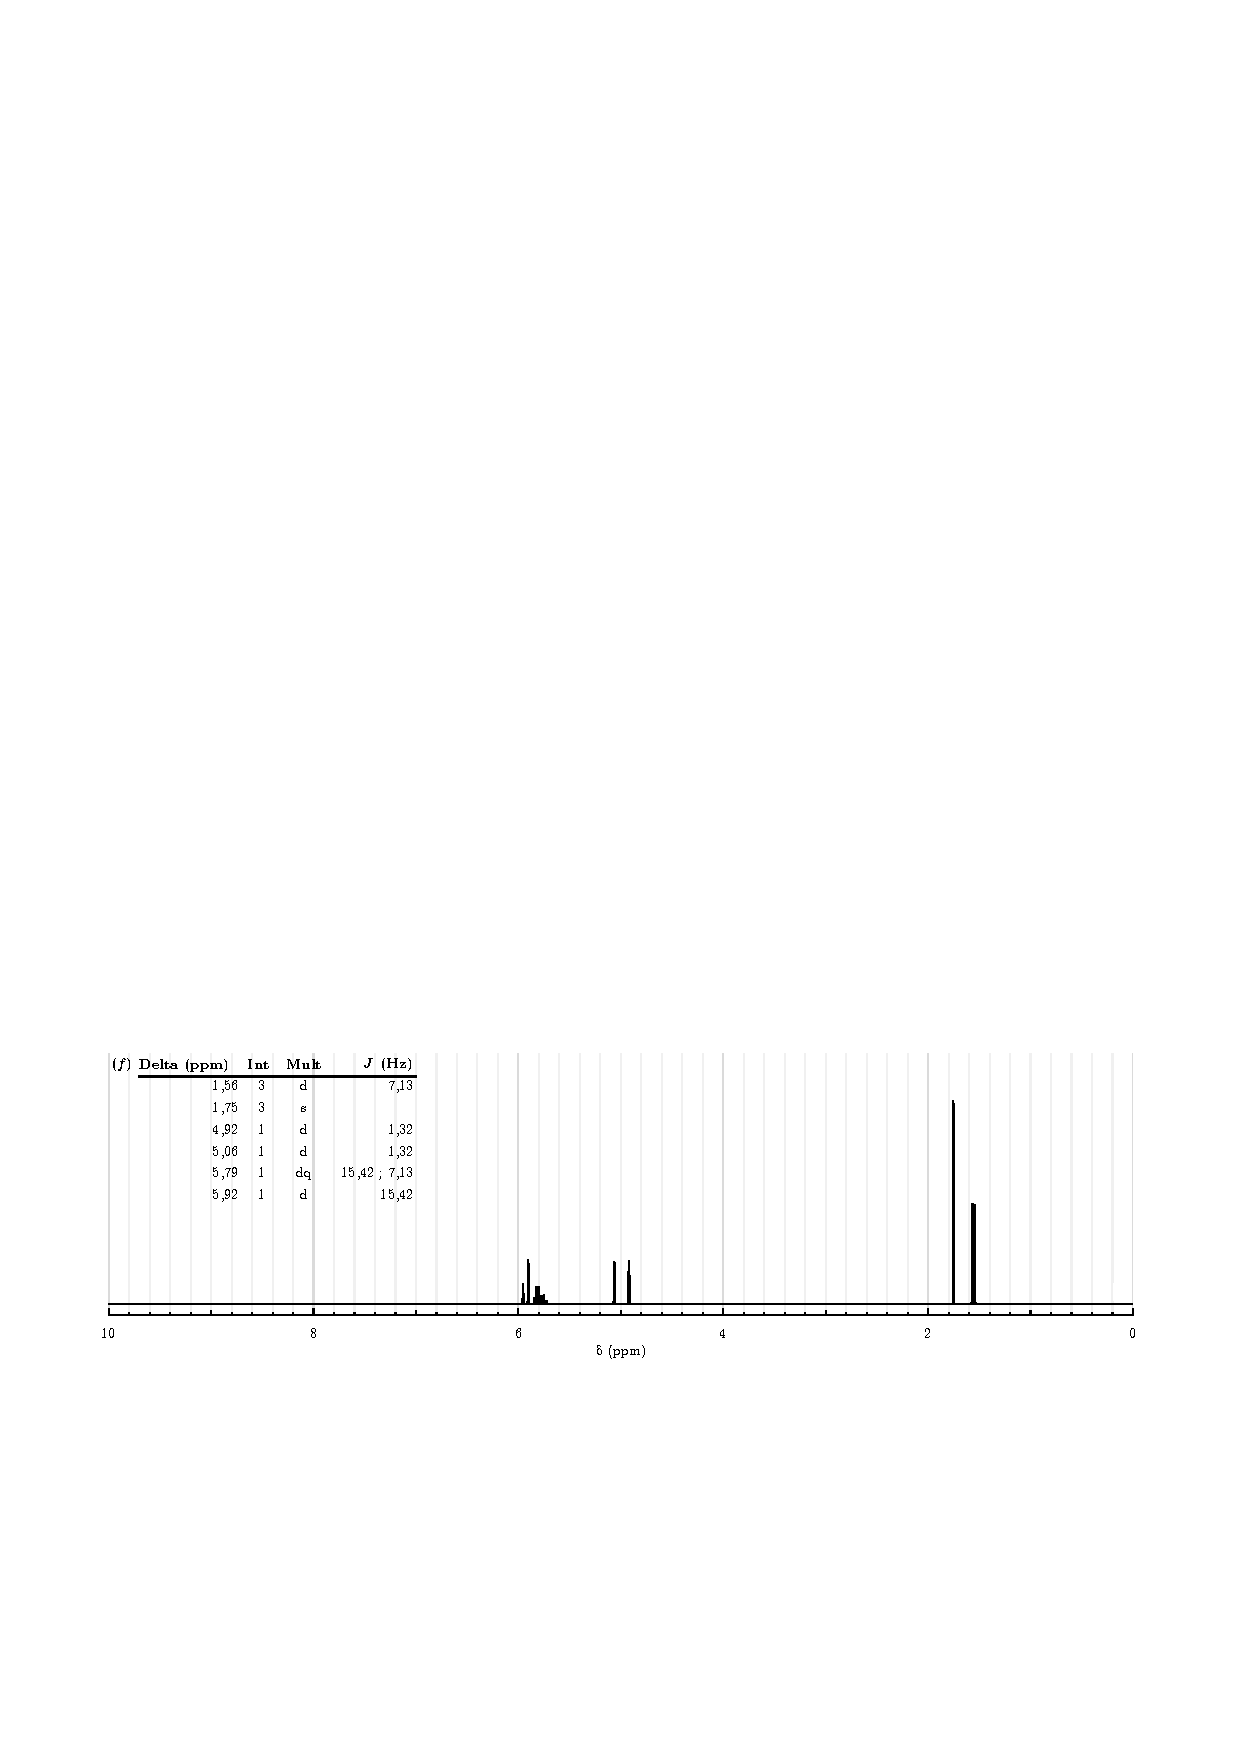
\includegraphics[width=.95\linewidth]{chimiePC/orga/RMN_3E-2.pdf}
    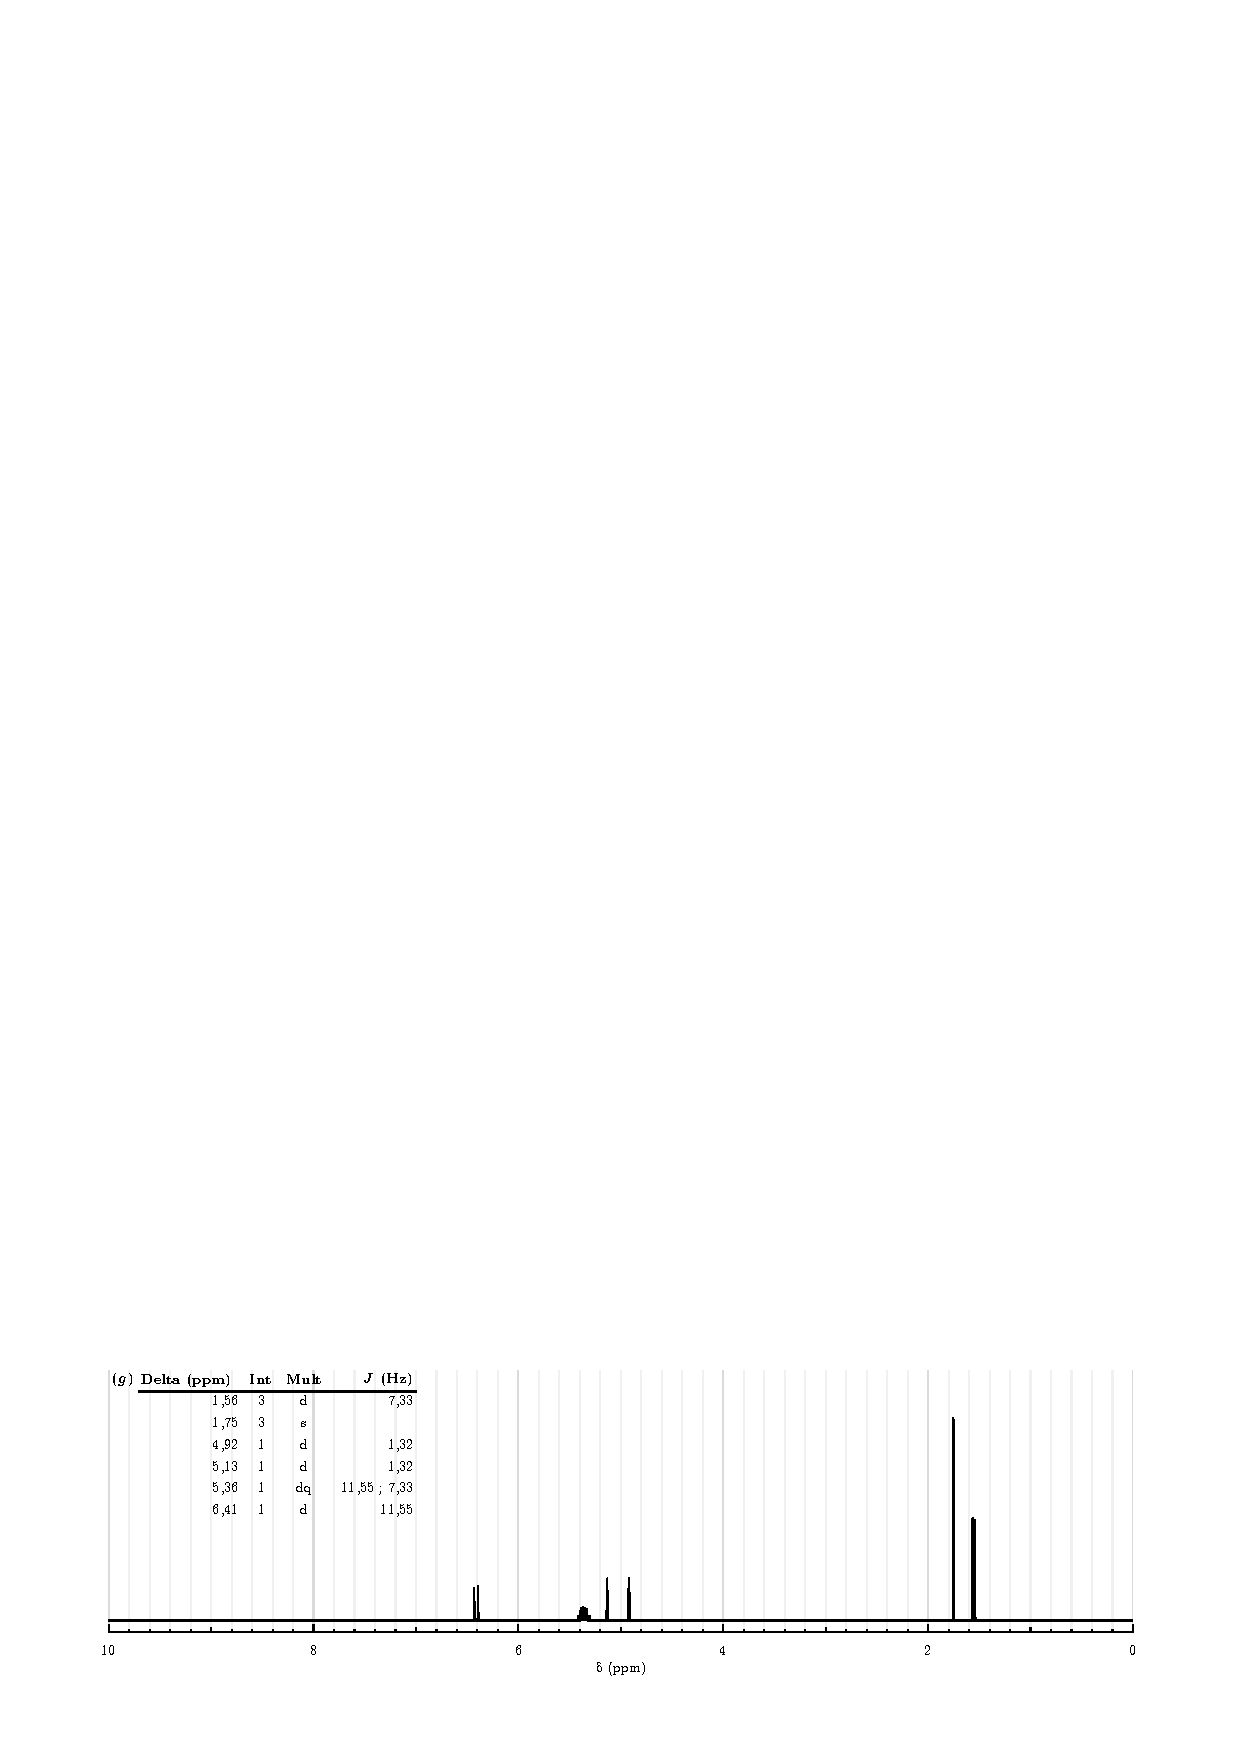
\includegraphics[width=.95\linewidth]{chimiePC/orga/RMN_3Z-2.pdf}
    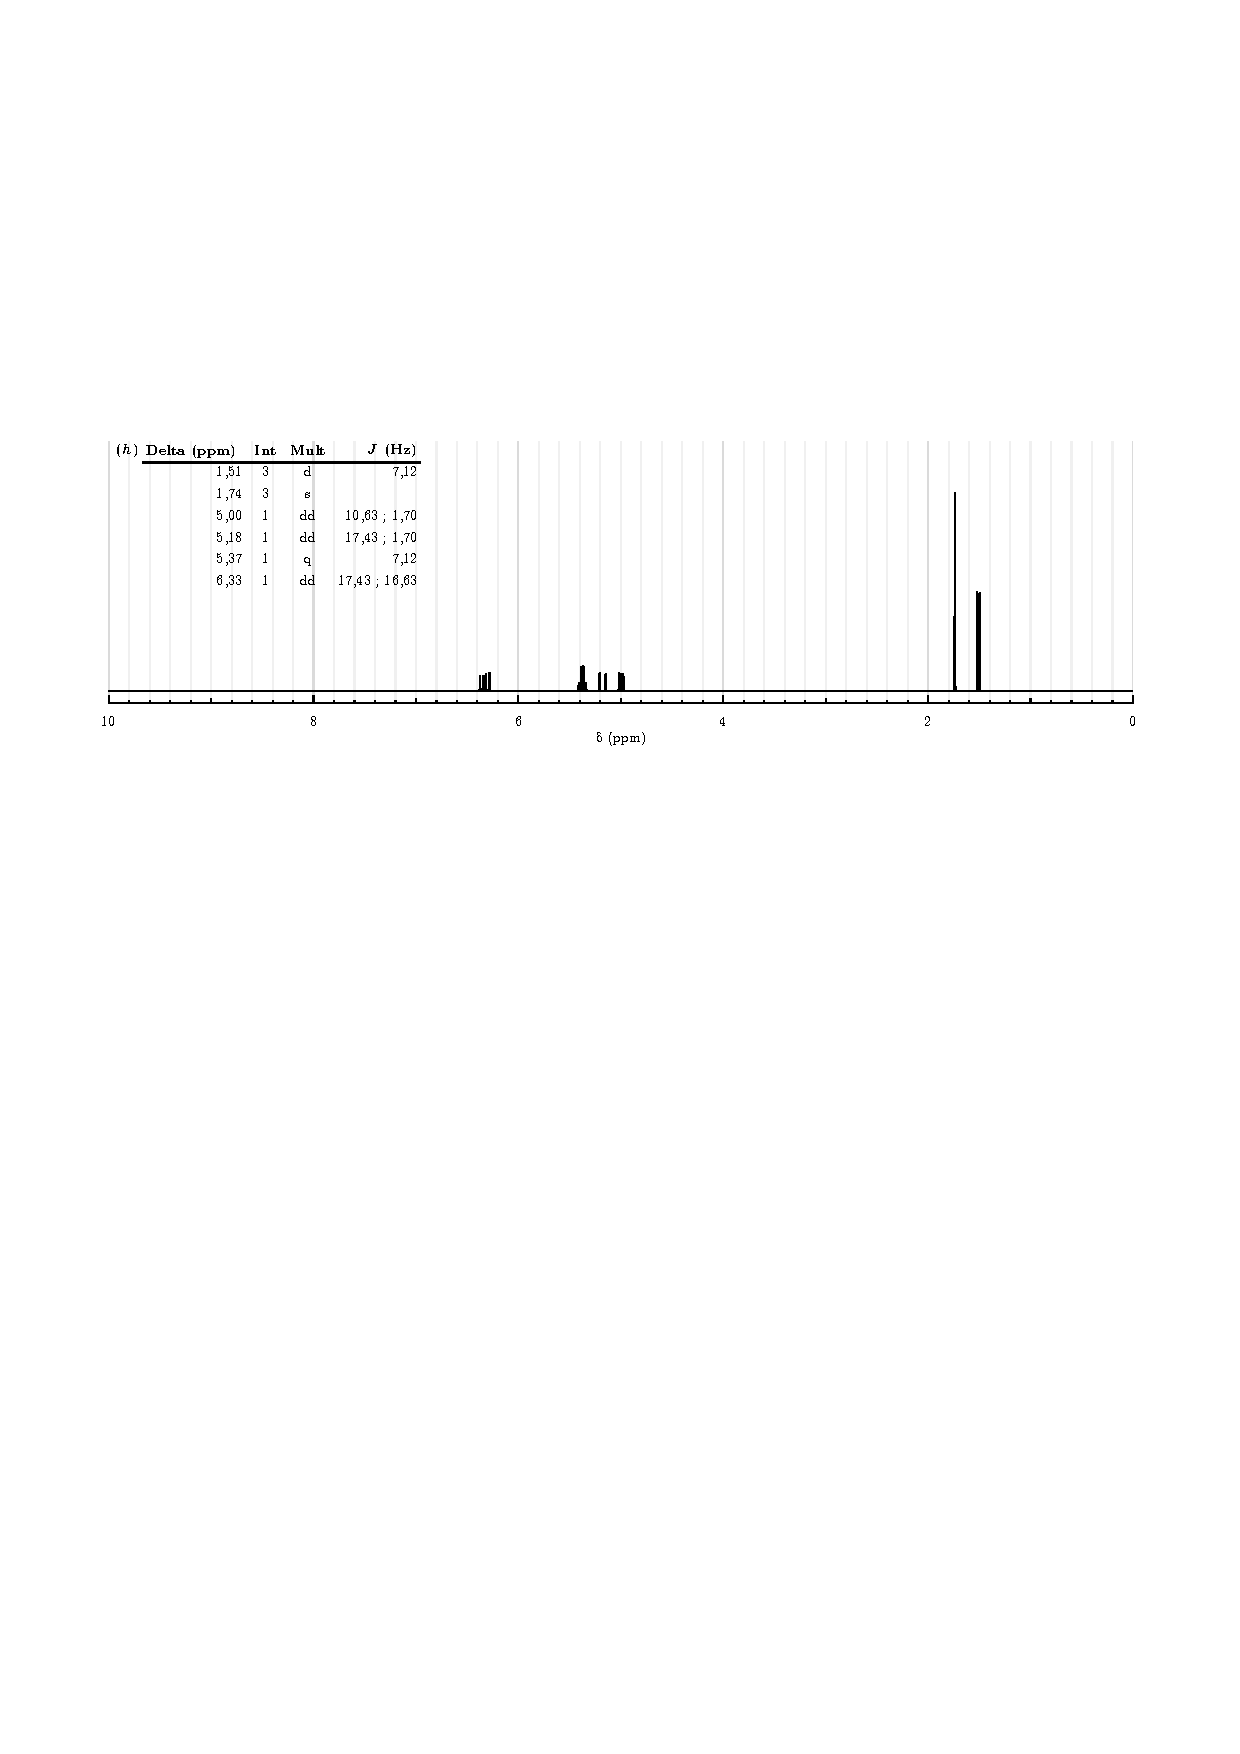
\includegraphics[width=.95\linewidth]{chimiePC/orga/RMN_3E-3.pdf}
    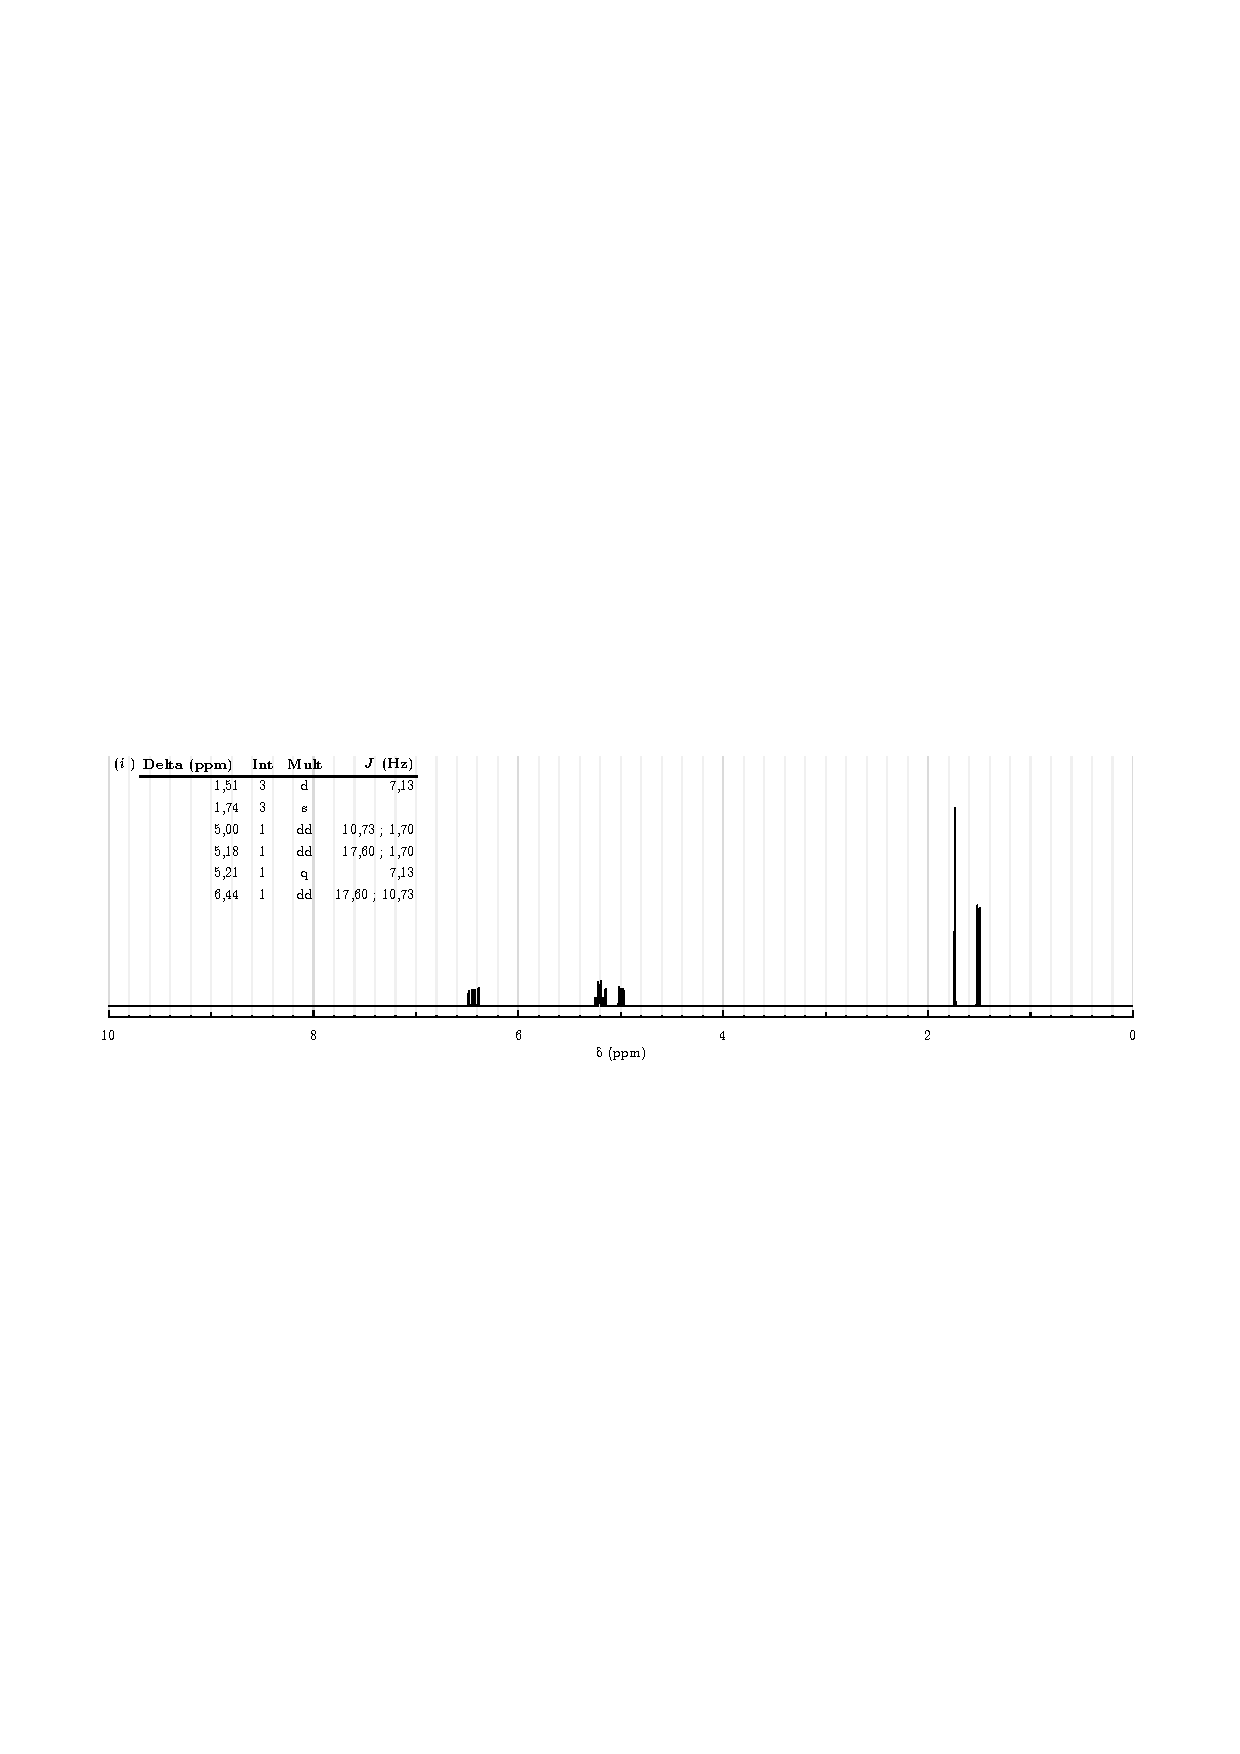
\includegraphics[width=.95\linewidth]{chimiePC/orga/RMN_3Z-3.pdf}
\end{center}

\begin{solution}
\begin{questions}
    \questioncours Multiplicité, topicité...
    
    \question 
    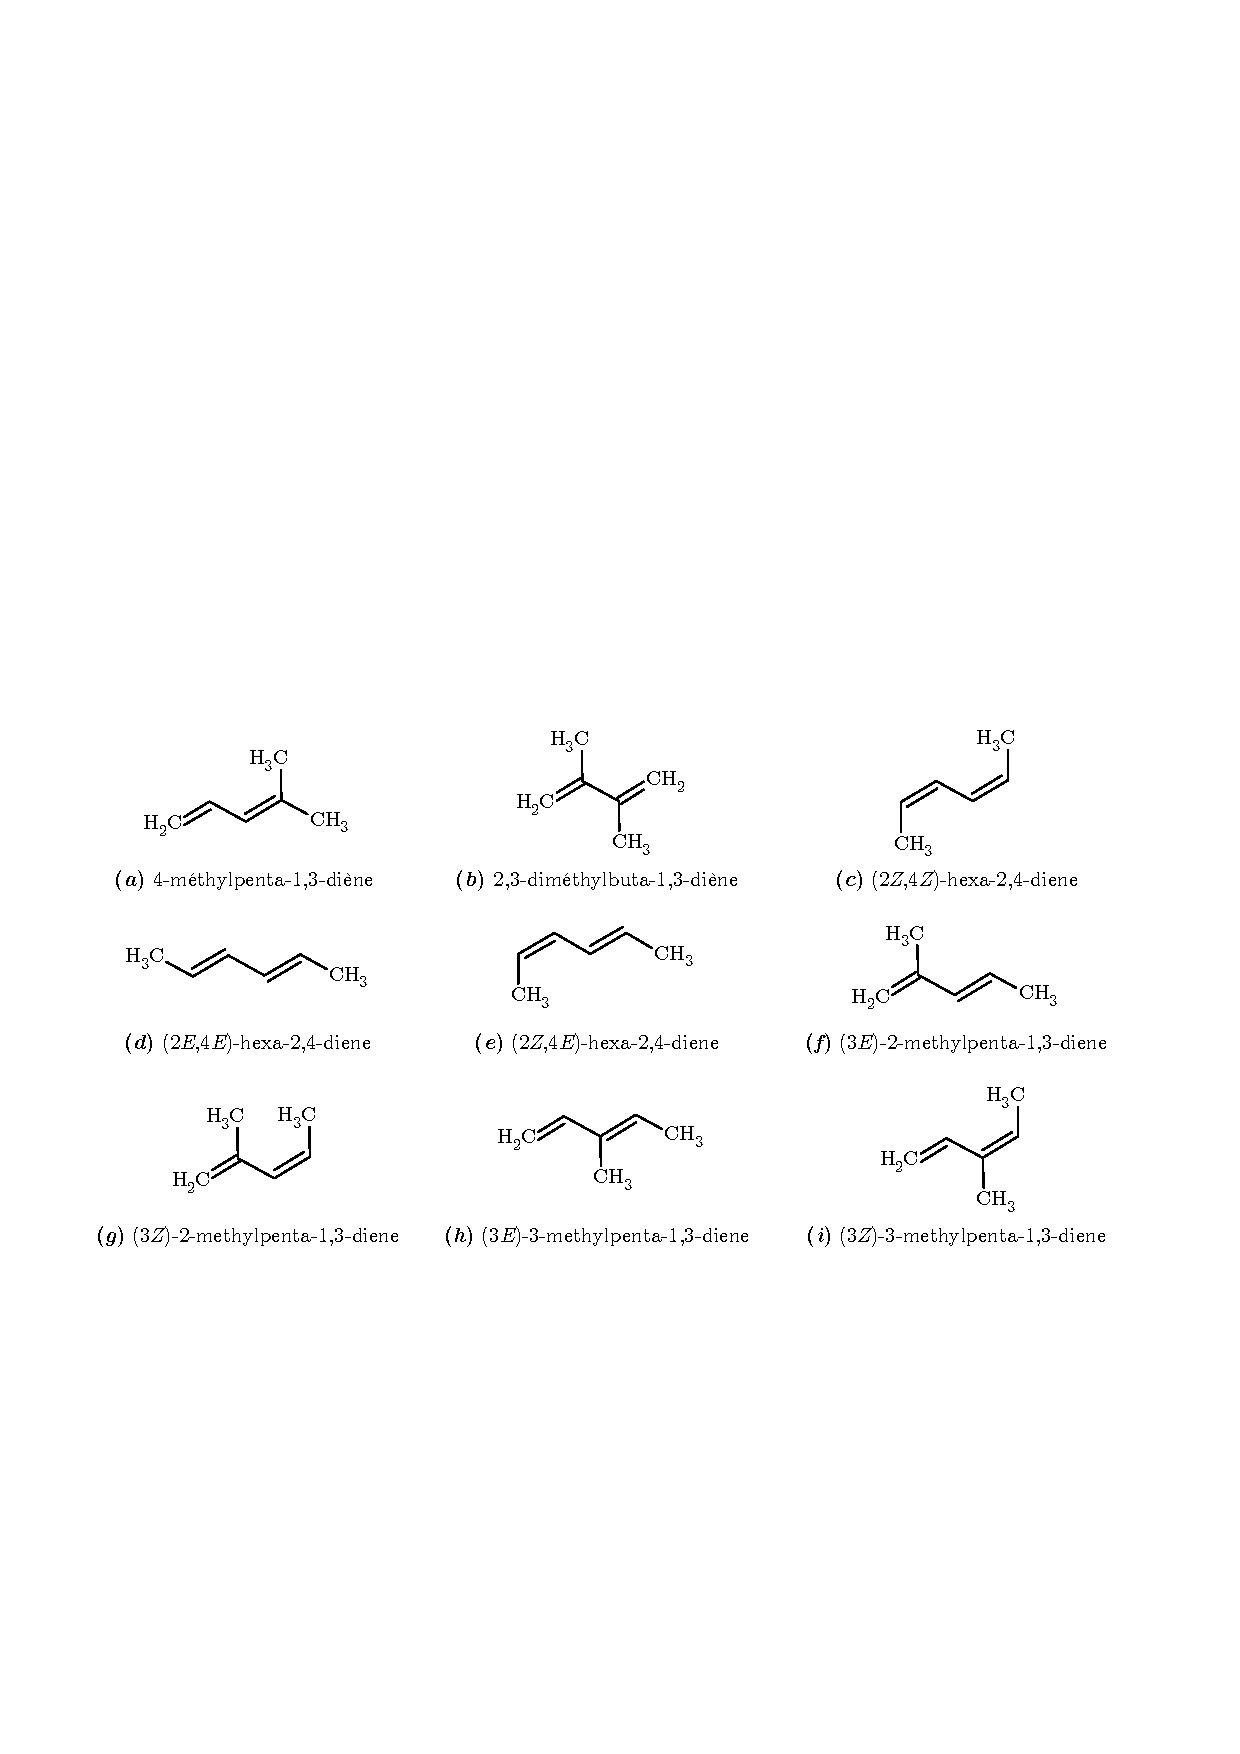
\includegraphics[width=.99\linewidth]{chimiePC/orga/RMN_sols.pdf}
\end{questions}
\end{solution}
% Niveau :      PCSI *
% Discipline :  Chimie Orga
% Mots clés :   Stéréochimie

\begin{exercise}{\'Equilibre céto-énolique et RMN}{2}{PCSI}
{Chimie organique I,Spectroscopie,RMN,Tautomérie}{bermu}

\begin{questions}
\questioncours RMN du proton $^{1}$H. Réalisation d'un spectre, principe de fonctionnement. Déplacement chimique $\delta$ : influence de l'environnement chimique et du solvant.

\begin{figure}[H]
    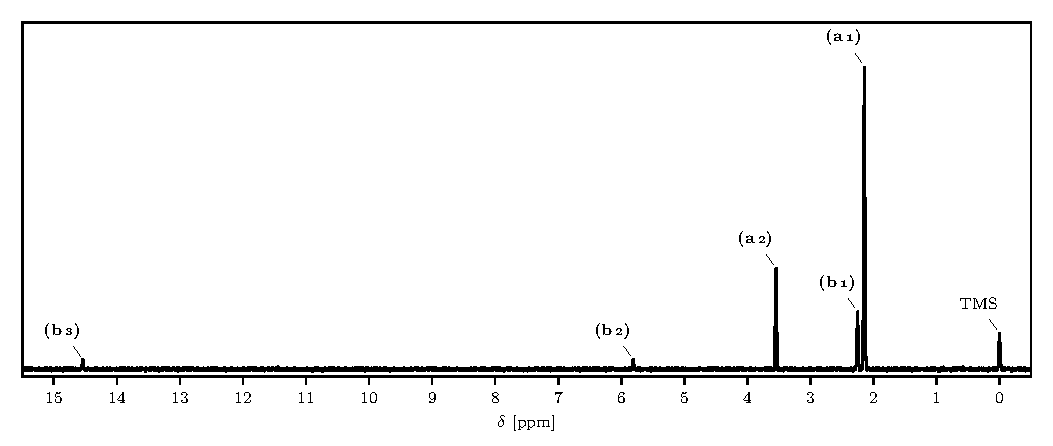
\includegraphics[width=\linewidth]{chimiePC/orga/keto1.pdf},
    \centering
    \begin{tabularx}{.7\linewidth}{c|l|CcCCCC}
        & & \multicolumn{6}{l}{\textbf{Intégration} pour différents solvants} \\
        & $\boldsymbol{\delta}$ \textbf{[ppm]} & $\mathrm{D_2O}$ & $\mathrm{DMSO}$-$d_6$ & $\mathrm{D_3COD}$ & Pur & $\mathrm{DCC\ell_3}$ & $\mathrm{C_6D_{12}}$ \\ \hline\hline
        \textbf{(a{\tiny\,1})} & $2.14$ & $1.00$ & $0.61$ & $0.35$ & $0.23$ & $0.05$ & $0.03$ \\
        \textbf{(a{\tiny\,2})} & $3.54$ & $0.33$ & $0.20$ & $0.12$ & $0.08$ & $0.02$ & $0.01$ \\
        \textbf{(b{\tiny\,1})} & $2.25$ & $0.19$ & $1.00$ & $1.00$ & $1.00$ & $1.00$ & $1.00$ \\
        \textbf{(b{\tiny\,2})} & $5.81$ & $0.03$ & $0.17$ & $0.17$ & $0.17$ & $0.17$ & $0.17$ \\
        \textbf{(b{\tiny\,3})} & $14.54$ & $0.03$ & $0.17$ & $0.17$ & $0.17$ & $0.17$ & $0.17$ \\\hline
    \end{tabularx}
    \caption{Spectres RMN $^{1}$H à 600 Hz du composé $\mathrm{C_5H_8O_2}$ réalisés dans différents solvants. \newline Le spectre tracé est effectué dans $\mathrm{D_2O}$.}
\end{figure}

\question \'Etant donné le spectre RMN ci-dessus, retrouver la structure du composé \textbf{A} de formule brute $\mathrm{C_5H_8O_2}$. On ne prendra en compte que les pics numérotés $\textbf{(a\,i)}$.

\question La présence du second groupe de pics, notés $\textbf{(b\,i)}$, est due à un second composé \textbf{B} en équilibre avec \textbf{A}, $\textbf{A} \xrightleftharpoons{} \textbf{B}.$ \\
Quelle est la structure de \textbf{B} ?

\question Commenter le déplacement chimique du pic \textbf{(b{\tiny\,3})}. Connaissez-vous d'autres fonctions qui ont un déplacement aussi élevé ? Pourquoi utiliser des solvants deutérés ?

\question \`A partir de la table d'intégration, donnez la fraction molaire $x_\textbf{A}$ de \textbf{A} pour chaque solvant.

\question Commenter l'évolution de $x_\textbf{A}$ dans chaque sovlant.
\end{questions}

\plusloin Discuter des constantes de vitesse de la réaction $\textbf{A} \xrightleftharpoons{} \textbf{B}$ par rapport à la résolution en fréquence de l'appareil.

\end{exercise}
% Niveau :      PCSI *
% Discipline :  Chimie Orga
% Mots clés :   Stéréochimie

\begin{exercise}{Spectre RMN des acides aminés}{2}{PCSI}
{Chimie organique I,Spectroscopie,RMN}{bermu}

\begin{questions}
\questioncours Couplage spin-spin $^{2}J$, $^{3}J$ et $^{4}J$ en RMN du proton $^{1}$H. \\
On prendra soin d'expliquer l'origine du phénomène sur un exemple simple et d'énoncer des facteurs d'influence de la valeur de $J$.

\begin{EnvUplevel}
    Un$\cdot$e étudiant$\cdot$e de chimie a synthétisé le composé ci-dessous mais a trouvé étrange le spectre RMN qu'elle a obtenu :
    
    \noindent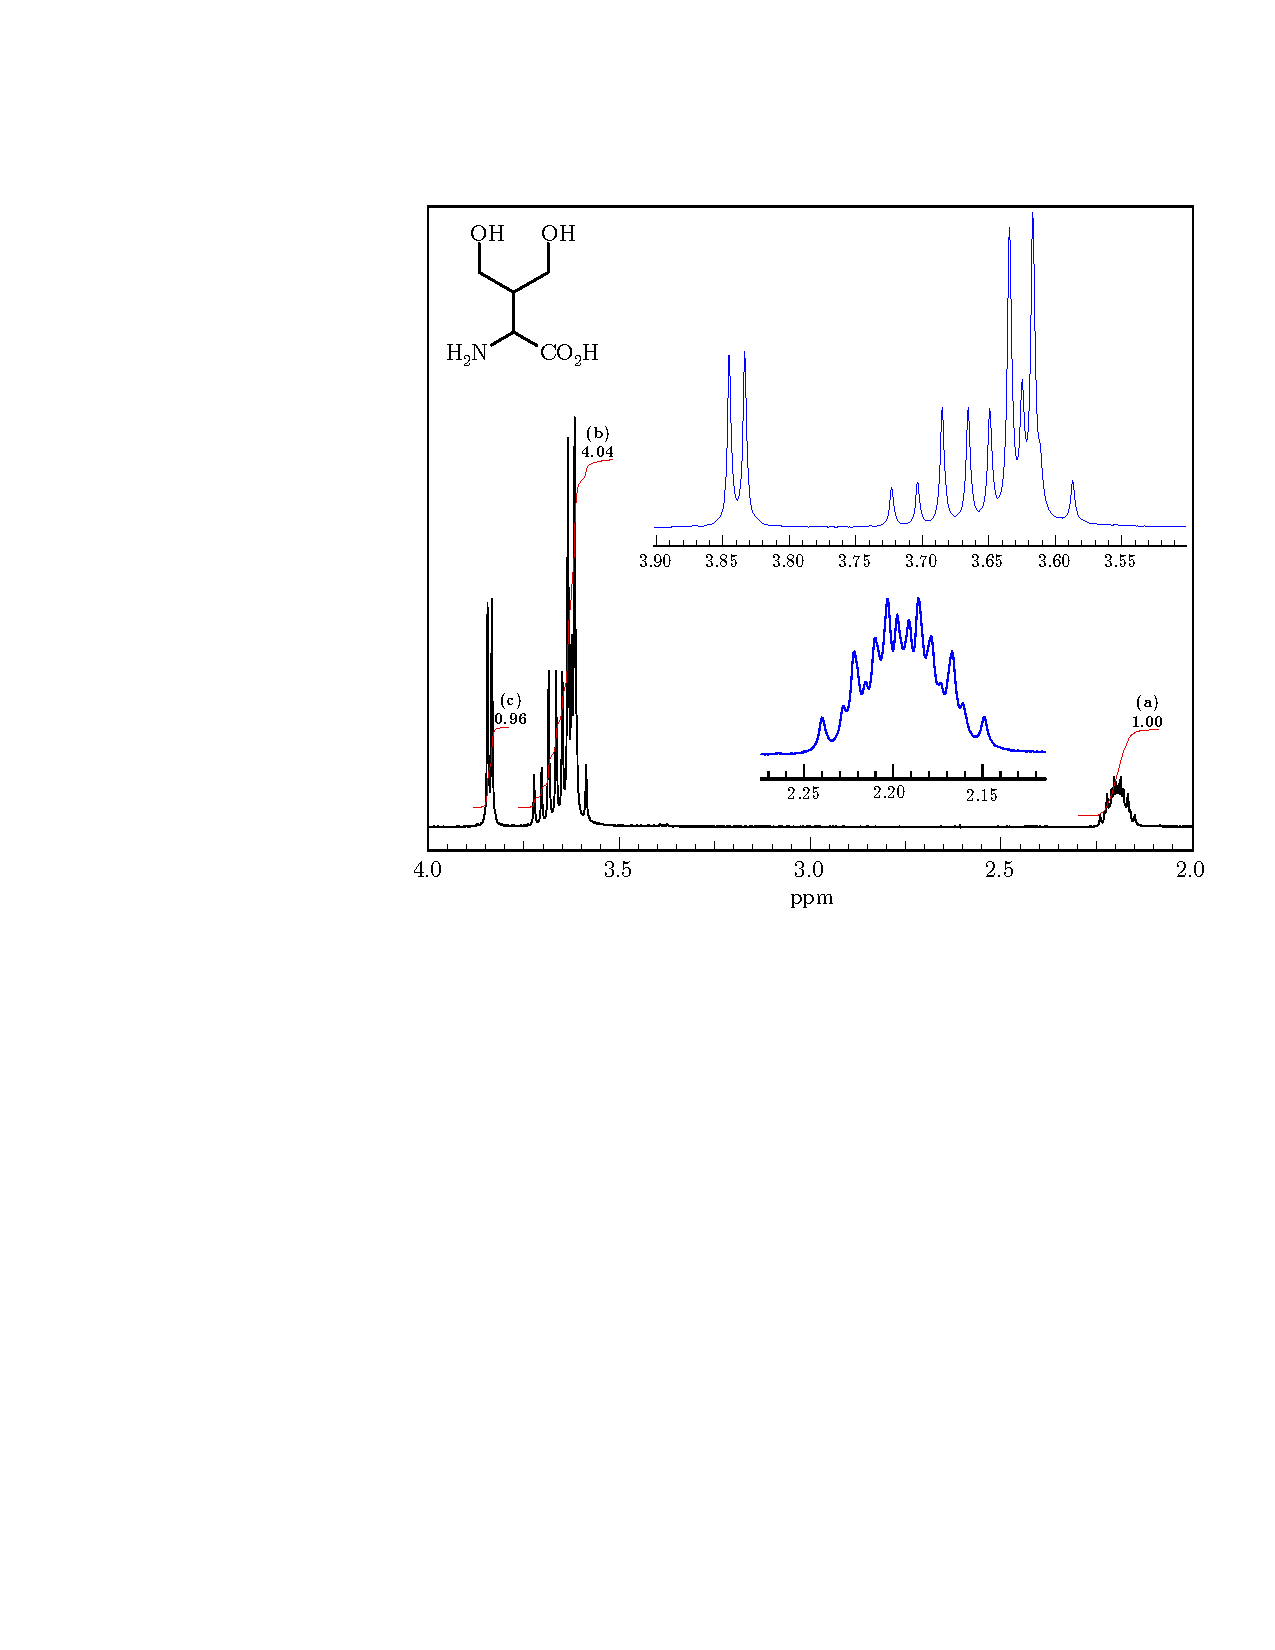
\includegraphics[width=\linewidth]{chimiePC/orga/acideamine.pdf}
    
    Le spectre RMN est effectué dans le $\mathrm{D_2O}$ à 300 MHz.
    
    Nous allons essayer de voir si l'étudiant$\cdot$e a bien synthétisé cette molécule ou non.
\end{EnvUplevel}

\question Identifiez chaque groupe de pics \textbf{(a)}, \textbf{(b)} et \textbf{(c)}.

\question Quels sont les différents couplages possibles ?

\question Calculez le couplage $J_c$ du doublet \textbf{(c)} et commentez sa valeur. \`A quoi correspond ce couplage ?

\question En essayant d'identifier des doublets dans le groupe \textbf{(b)}, attribuez les différents signaux aux couplages associés. On pourra s'aider de l'annexe du handbook.

\end{questions}


\end{exercise}
% Niveau :      PCSI *
% Discipline :  Chimie Orga
% Mots clés :   Stéréochimie

\begin{exercise}{Spectre RMN du [18]annulène}{3}{PCSI}
{Chimie organique I,Spectroscopie,RMN}{bermu}

\begin{questions}
\questioncours RMN du proton $^{1}$H. Réalisation d'un spectre, principe de fonctionnement. Déplacement chimique $\delta$ : influence de l'environnement chimique et du solvant.

\question Commentez les spectres RMN du [18]annulène :
\end{questions}

\noindent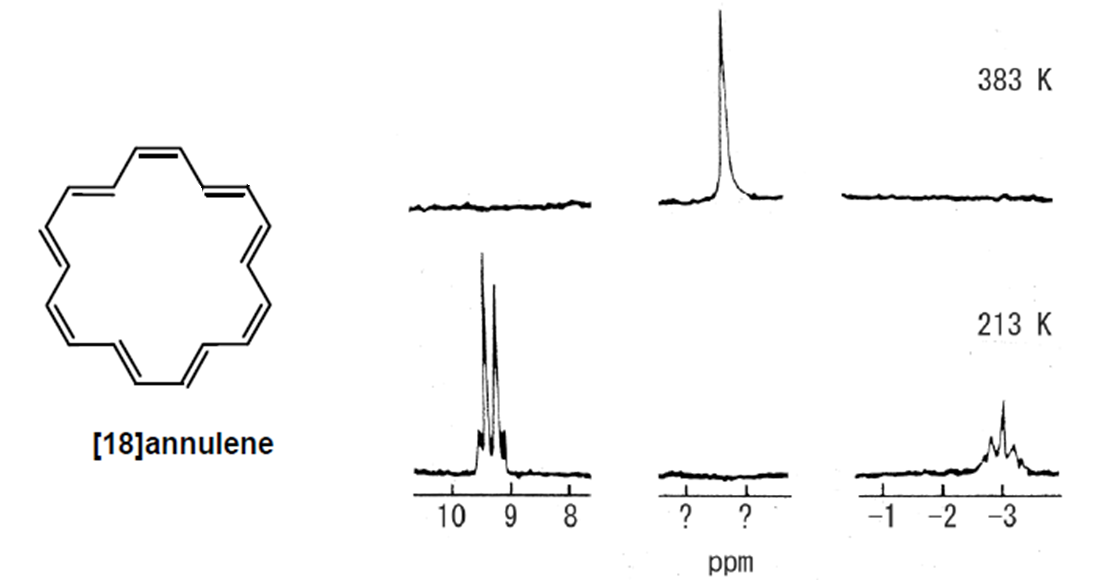
\includegraphics[width=\linewidth]{chimiePC/orga/annulene.png}

\end{exercise}
% Niveau :      PCSI *
% Discipline :  Chimie Orga
% Mots clés :   IR RMN

\begin{exercise}{Identification IR RMN 1}{1}{PCSI}
{Chimie organique I,Spectroscopie,RMN,Infrarouge}{bermu}

À l'aide des spectres IR et RMN $^{1}$H donnés ci-dessous, ainsi que des tables fournies en annexe, identifier la structure et attribuer les signaux spectroscopiques pertinents de ce composé de formule brute $\mathrm{C_{10}H_{14}O}$.
 
\vspace{2em}
 
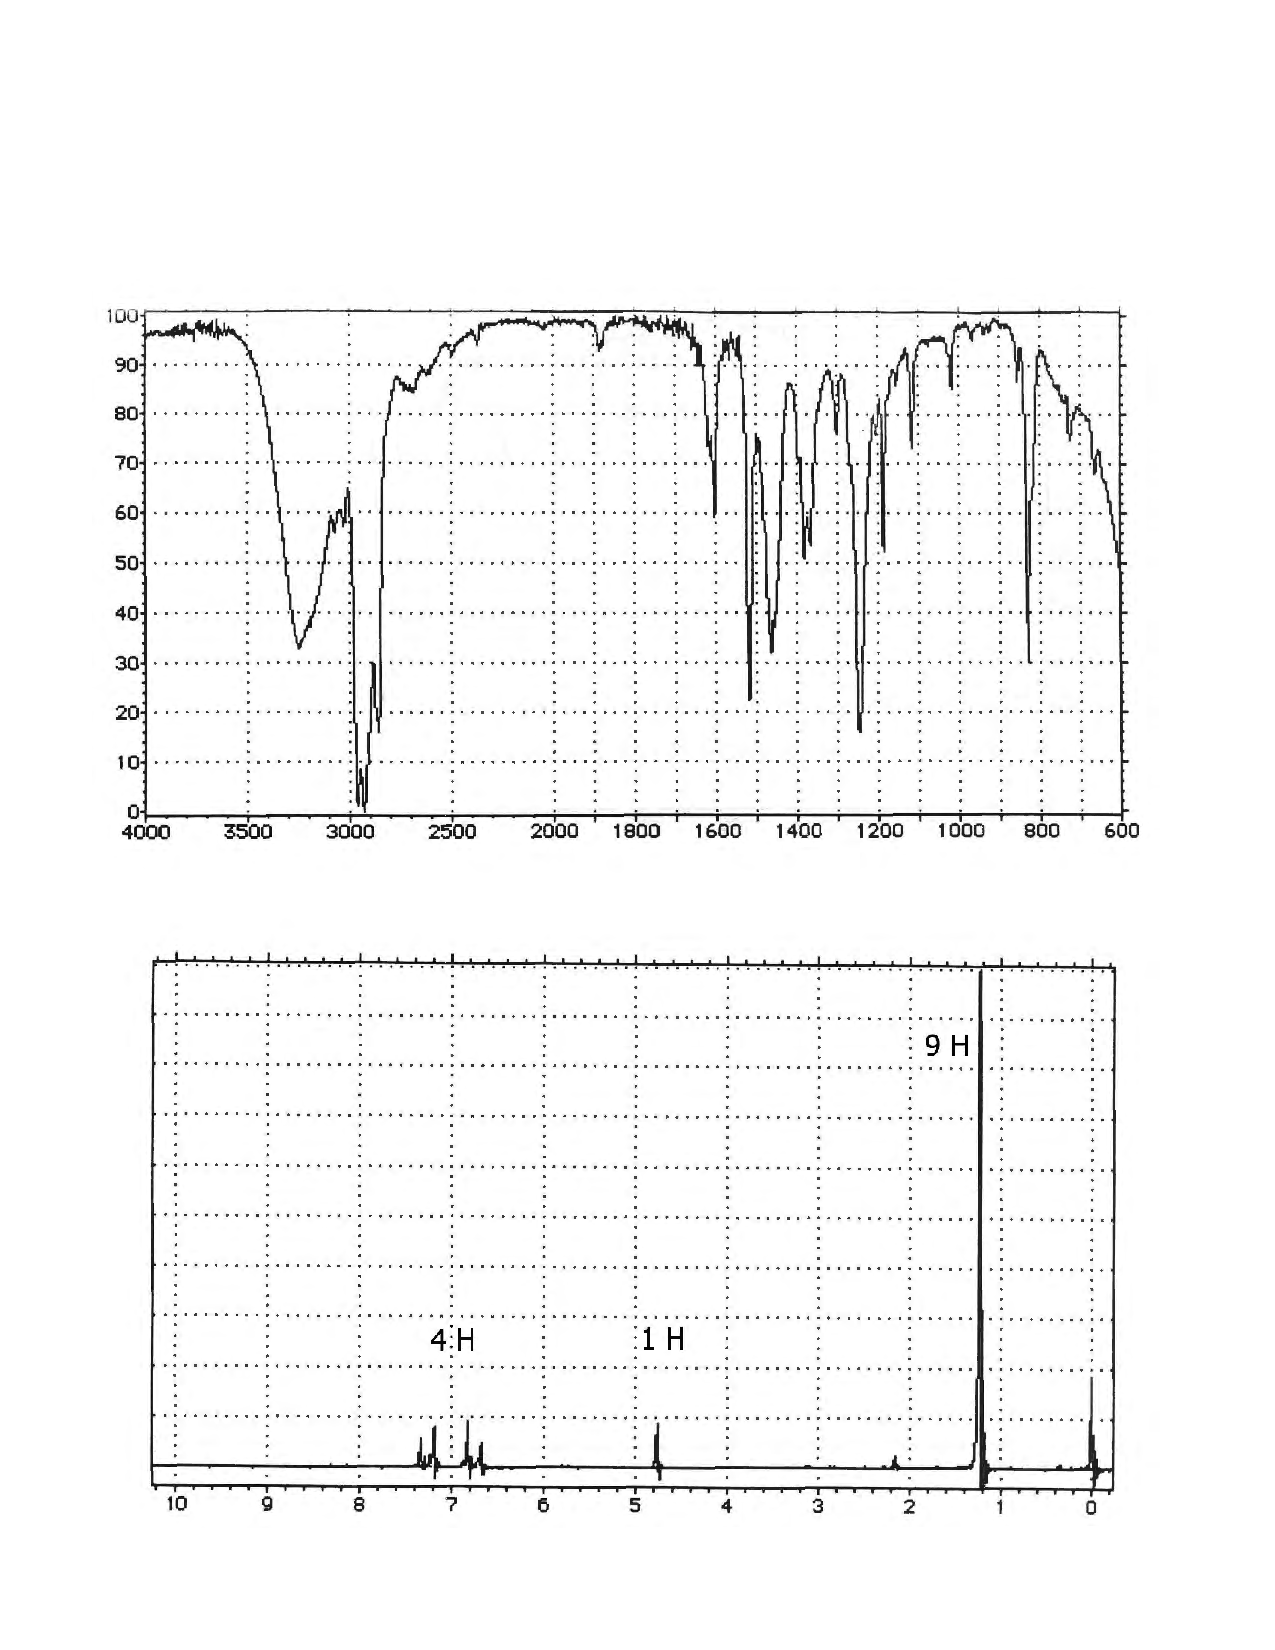
\includegraphics[width=\linewidth]{chimiePC/orga/IR_RMN_1.pdf}

\end{exercise}

\begin{solution}
\begin{center}
    \chemfig{HO-*6(=-=(-(-[:90]CH_3)(-CH_3)(-[:-90]CH_3))-=-)}
\end{center}
\end{solution}

\begin{exercise}{Identification IR RMN 2}{2}{PCSI}
{Chimie organique I,Spectroscopie,RMN,Infrarouge}{bermu}

À l'aide des spectres IR et RMN $^{1}$H donnés ci-dessous, ainsi que des tables fournies en annexe, identifier la structure et attribuer les signaux spectroscopiques pertinents de ce composé de formule brute $\mathrm{C_4H_{10}O_2}$.
 
\vspace{2em}
 
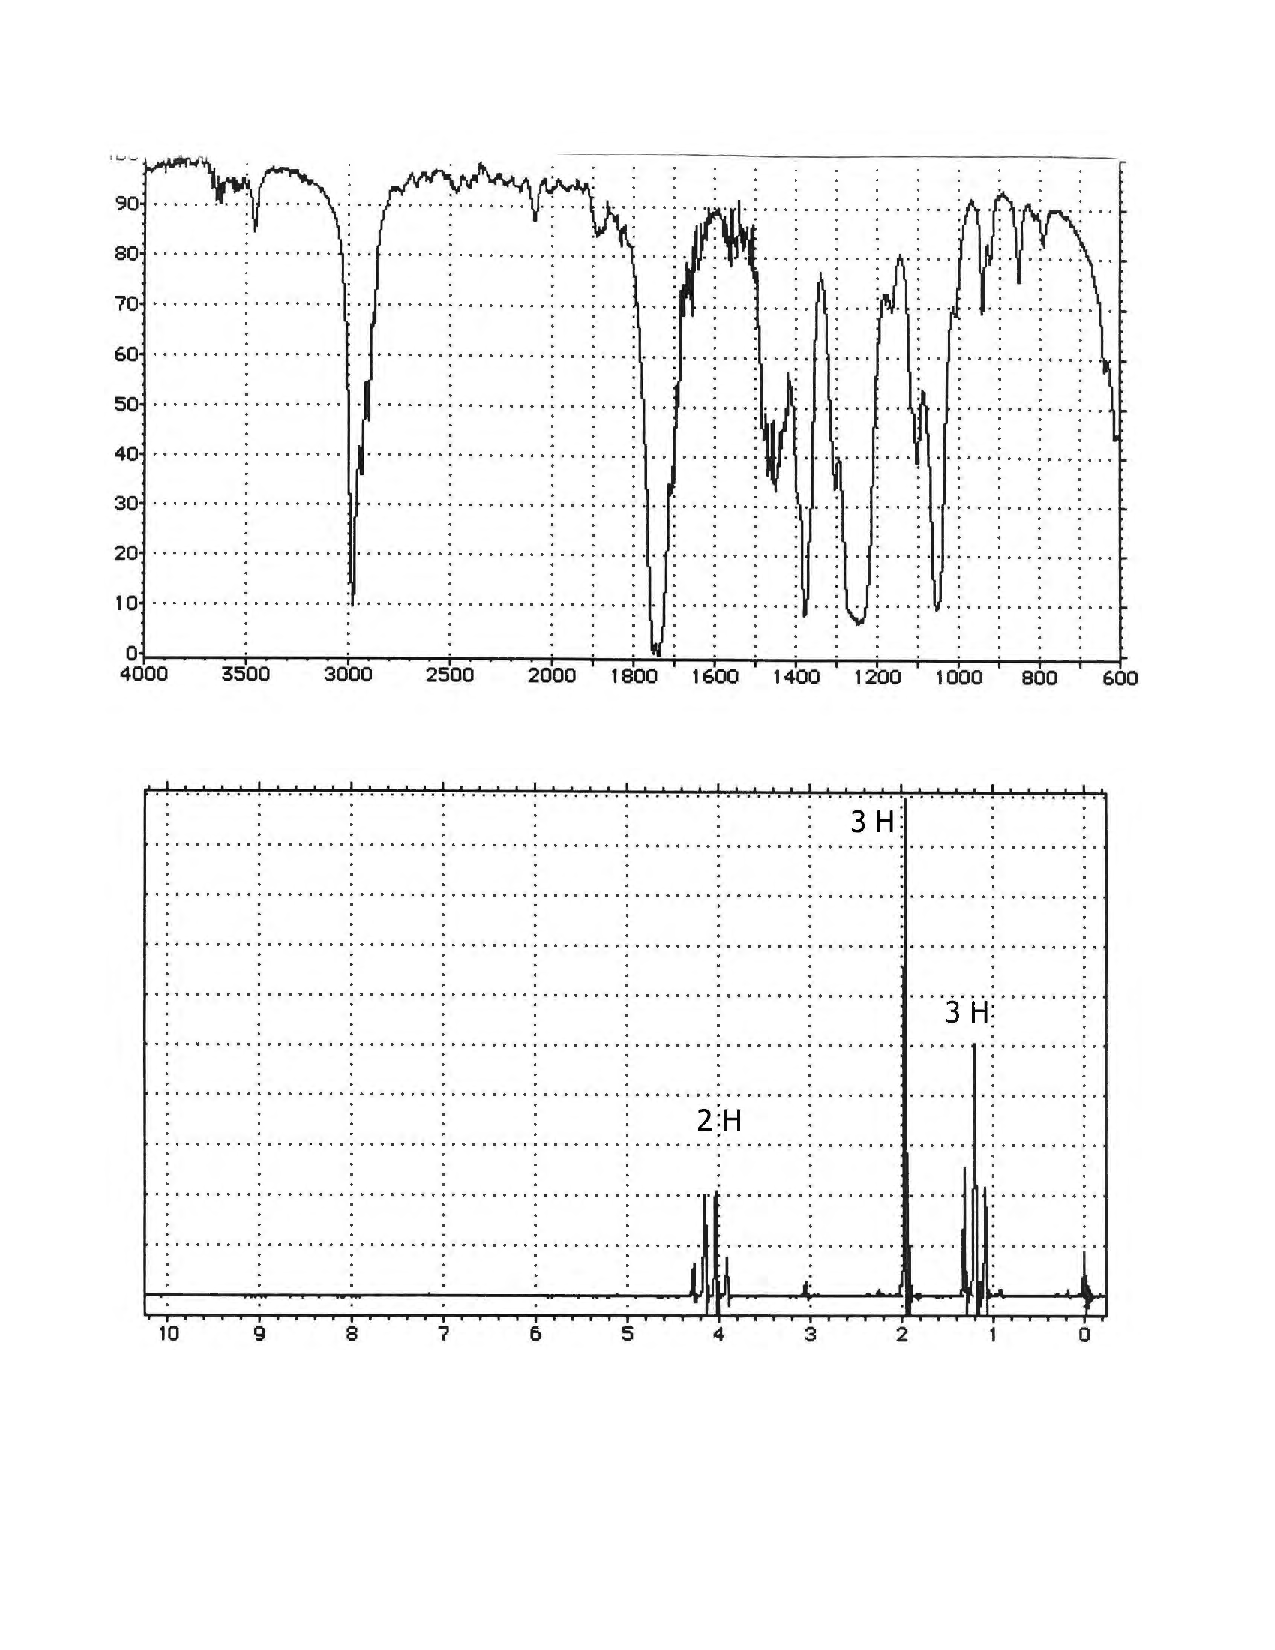
\includegraphics[width=\linewidth]{chimiePC/orga/IR_RMN_2.pdf}

\end{exercise}

\begin{solution}
\begin{center}
    \chemfig{-[1](=[3]O)-[-1]O-[1]-[-1]}
\end{center}
\end{solution}

\begin{exercise}{Identification IR RMN 3}{1}{PCSI}
{Chimie organique I,Spectroscopie,RMN,Infrarouge}{bermu}

À l'aide des spectres IR et RMN $^{1}$H donnés ci-dessous, ainsi que des tables fournies en annexe, identifier la structure et attribuer les signaux spectroscopiques pertinents de ce composé de formule brute $\mathrm{C_{10}H_{14}}$.
 
\vspace{2em}
 
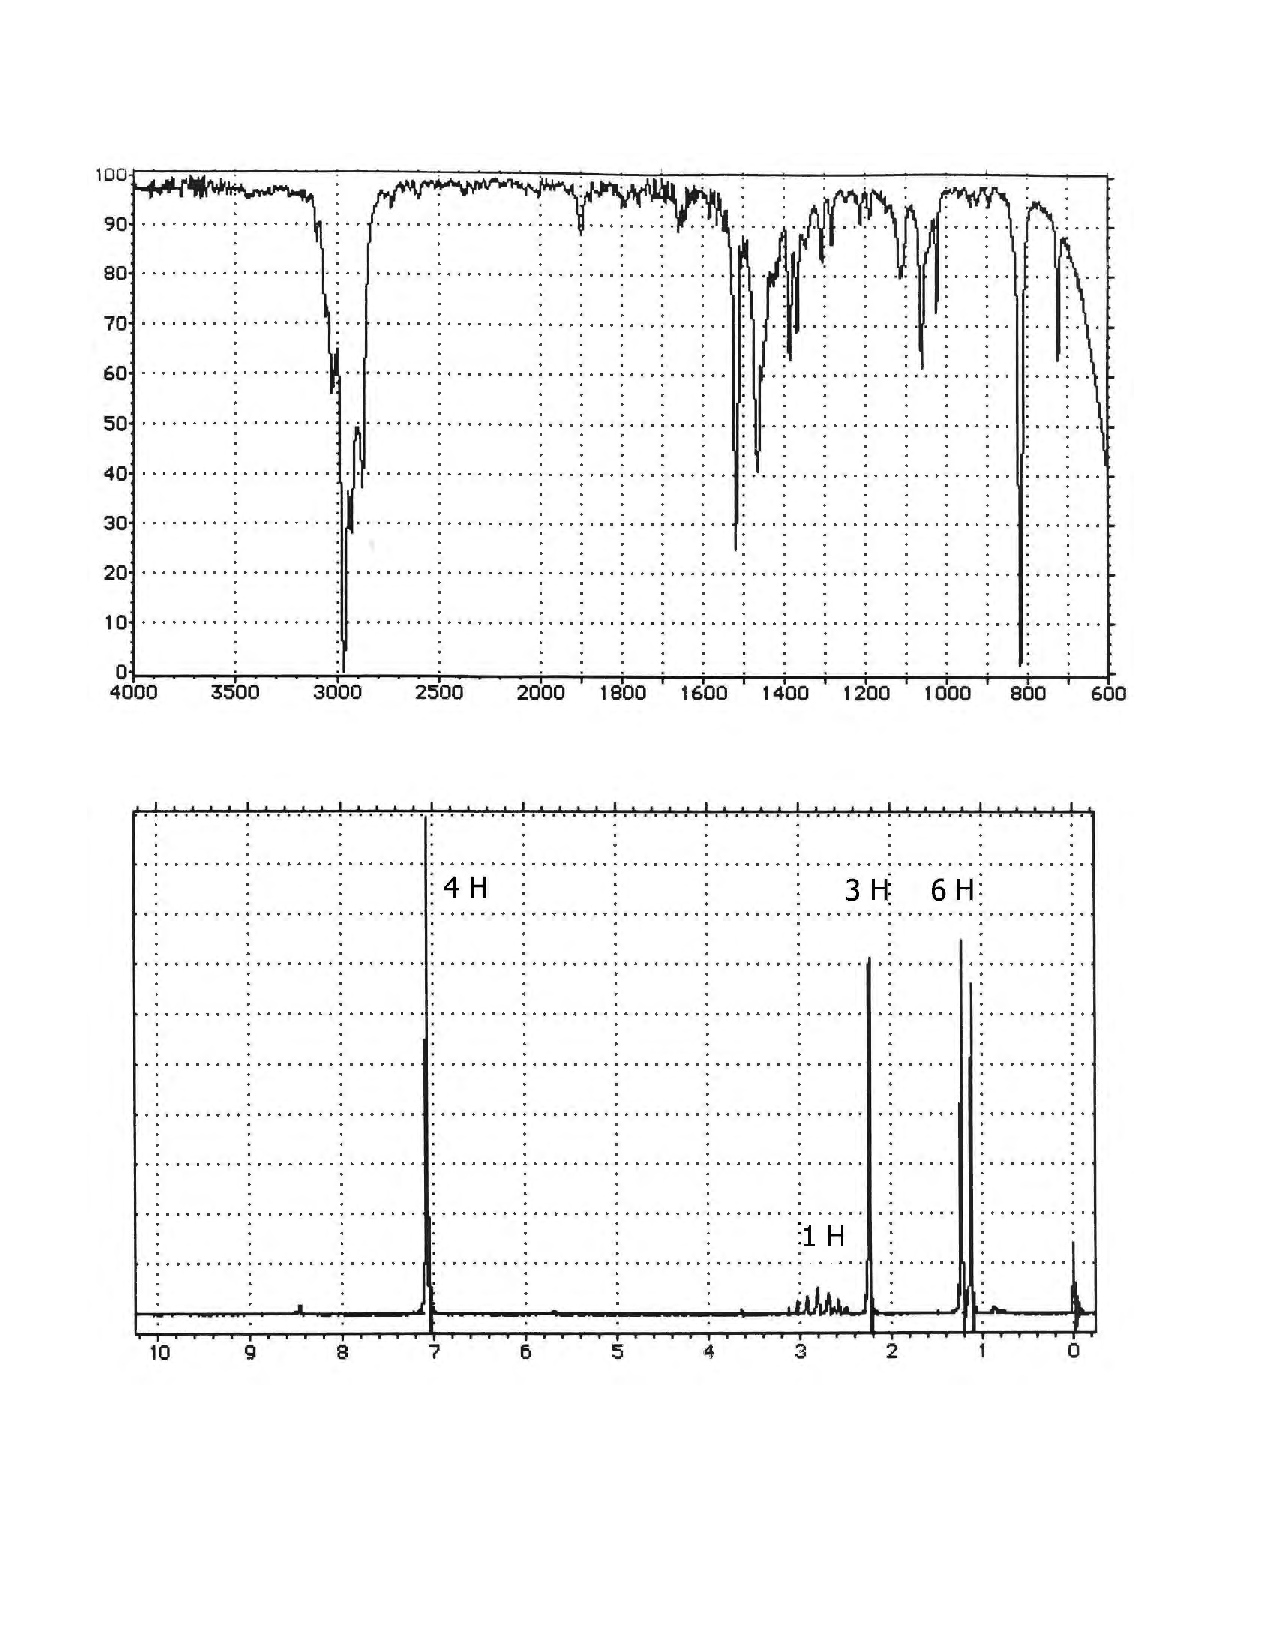
\includegraphics[width=\linewidth]{chimiePC/orga/IR_RMN_3.pdf}

\end{exercise}

\begin{solution}
\begin{center}
    \chemfig{H_3C-*6(=-=(-(-[2]CH_3)(-[-2]CH_3))-=-)}
\end{center}
\end{solution}

\begin{exercise}{Identification IR RMN 4}{2}{PCSI}
{Chimie organique I,Spectroscopie,RMN,Infrarouge}{bermu}

À l'aide des spectres IR et RMN $^{1}$H donnés ci-dessous, ainsi que des tables fournies en annexe, identifier la structure et attribuer les signaux spectroscopiques pertinents de ce composé de formule brute $\mathrm{C_9H_{10}O_2}$.
 
\vspace{2em}
 
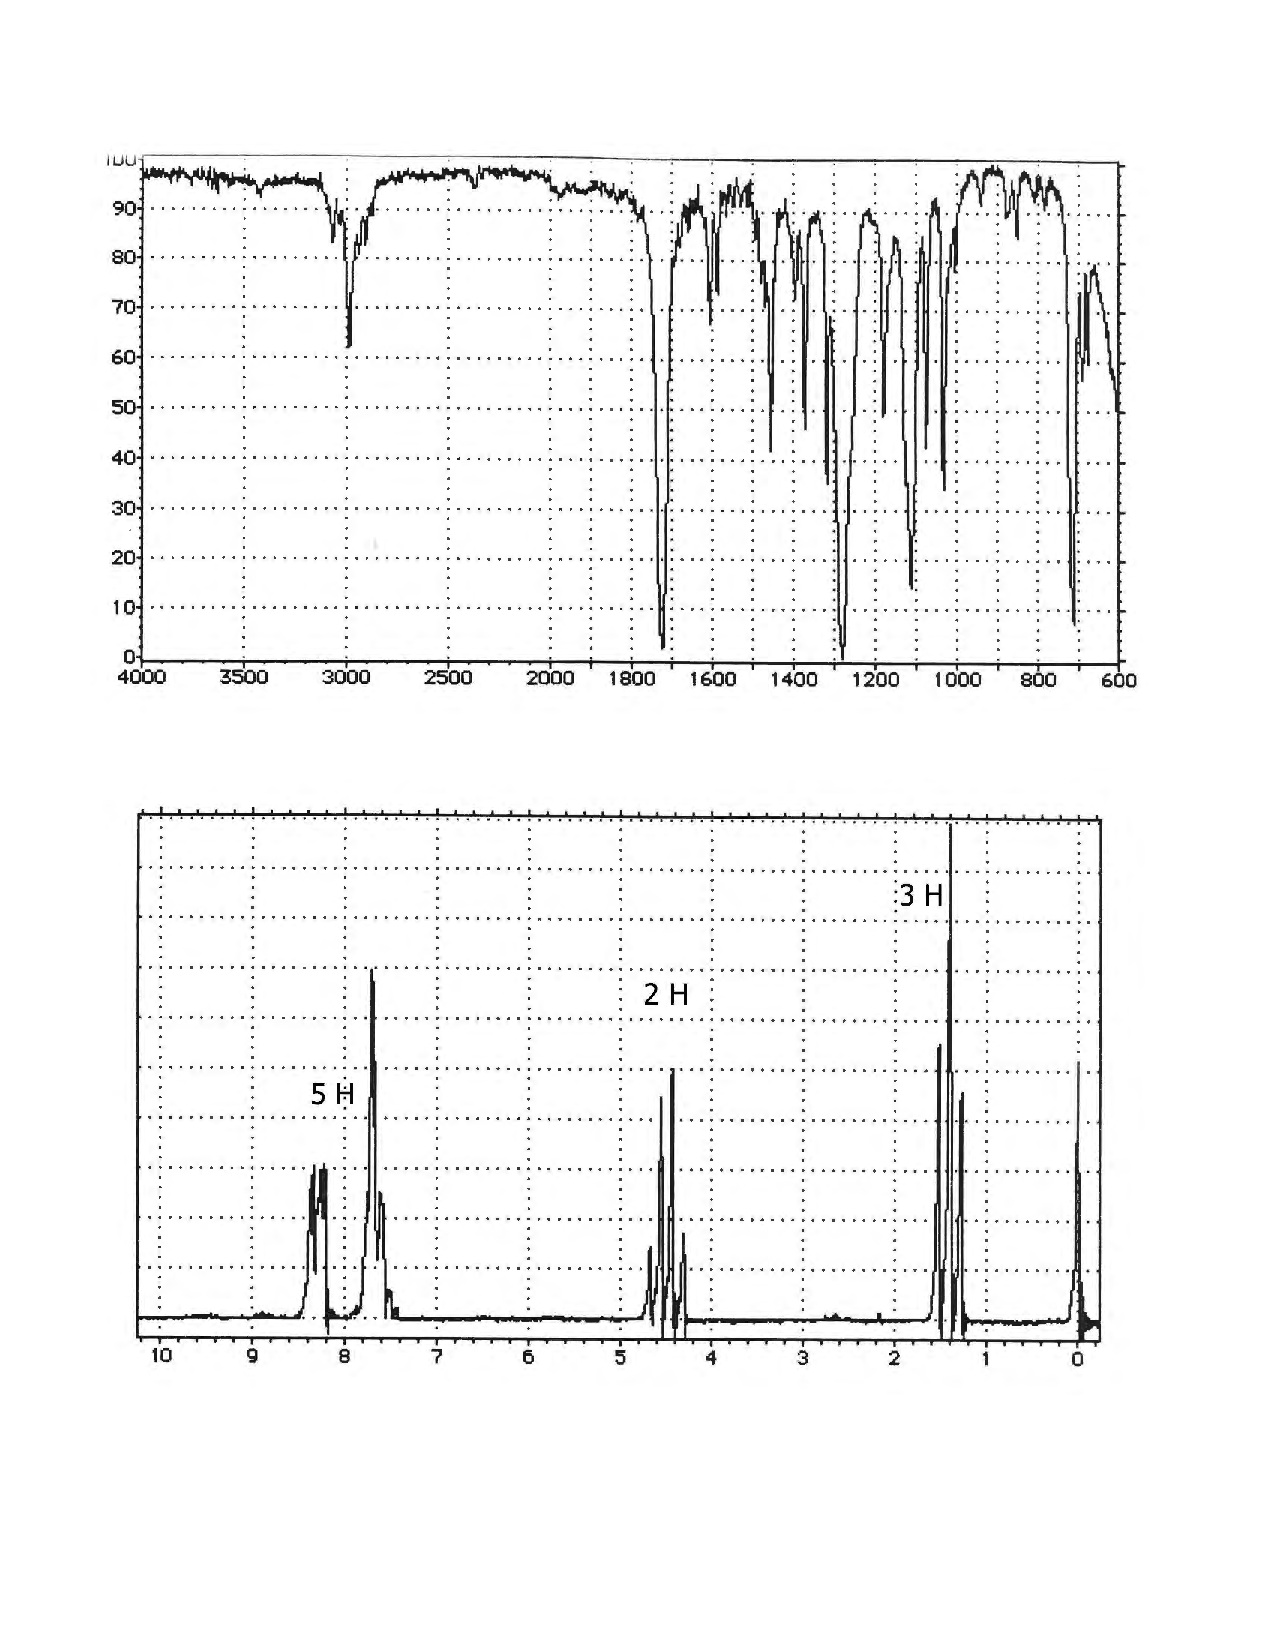
\includegraphics[width=\linewidth]{chimiePC/orga/IR_RMN_4.pdf}

\end{exercise}

\begin{solution}
\begin{center}
    \chemfig{[2]*6(=-(-[1](=[3]O)-[-1]O-[1]-[-1])=-=-)}
\end{center}
\end{solution}

\begin{exercise}{Identification IR RMN 5}{2}{PCSI}
{Chimie organique I,Spectroscopie,RMN,Infrarouge}{bermu}

À l'aide des spectres IR et RMN $^{1}$H donnés ci-dessous, ainsi que des tables fournies en annexe, identifier la structure et attribuer les signaux spectroscopiques pertinents de ce composé de formule brute $\mathrm{C_5H_{10}O_2}$.
 
\vspace{2em}
 
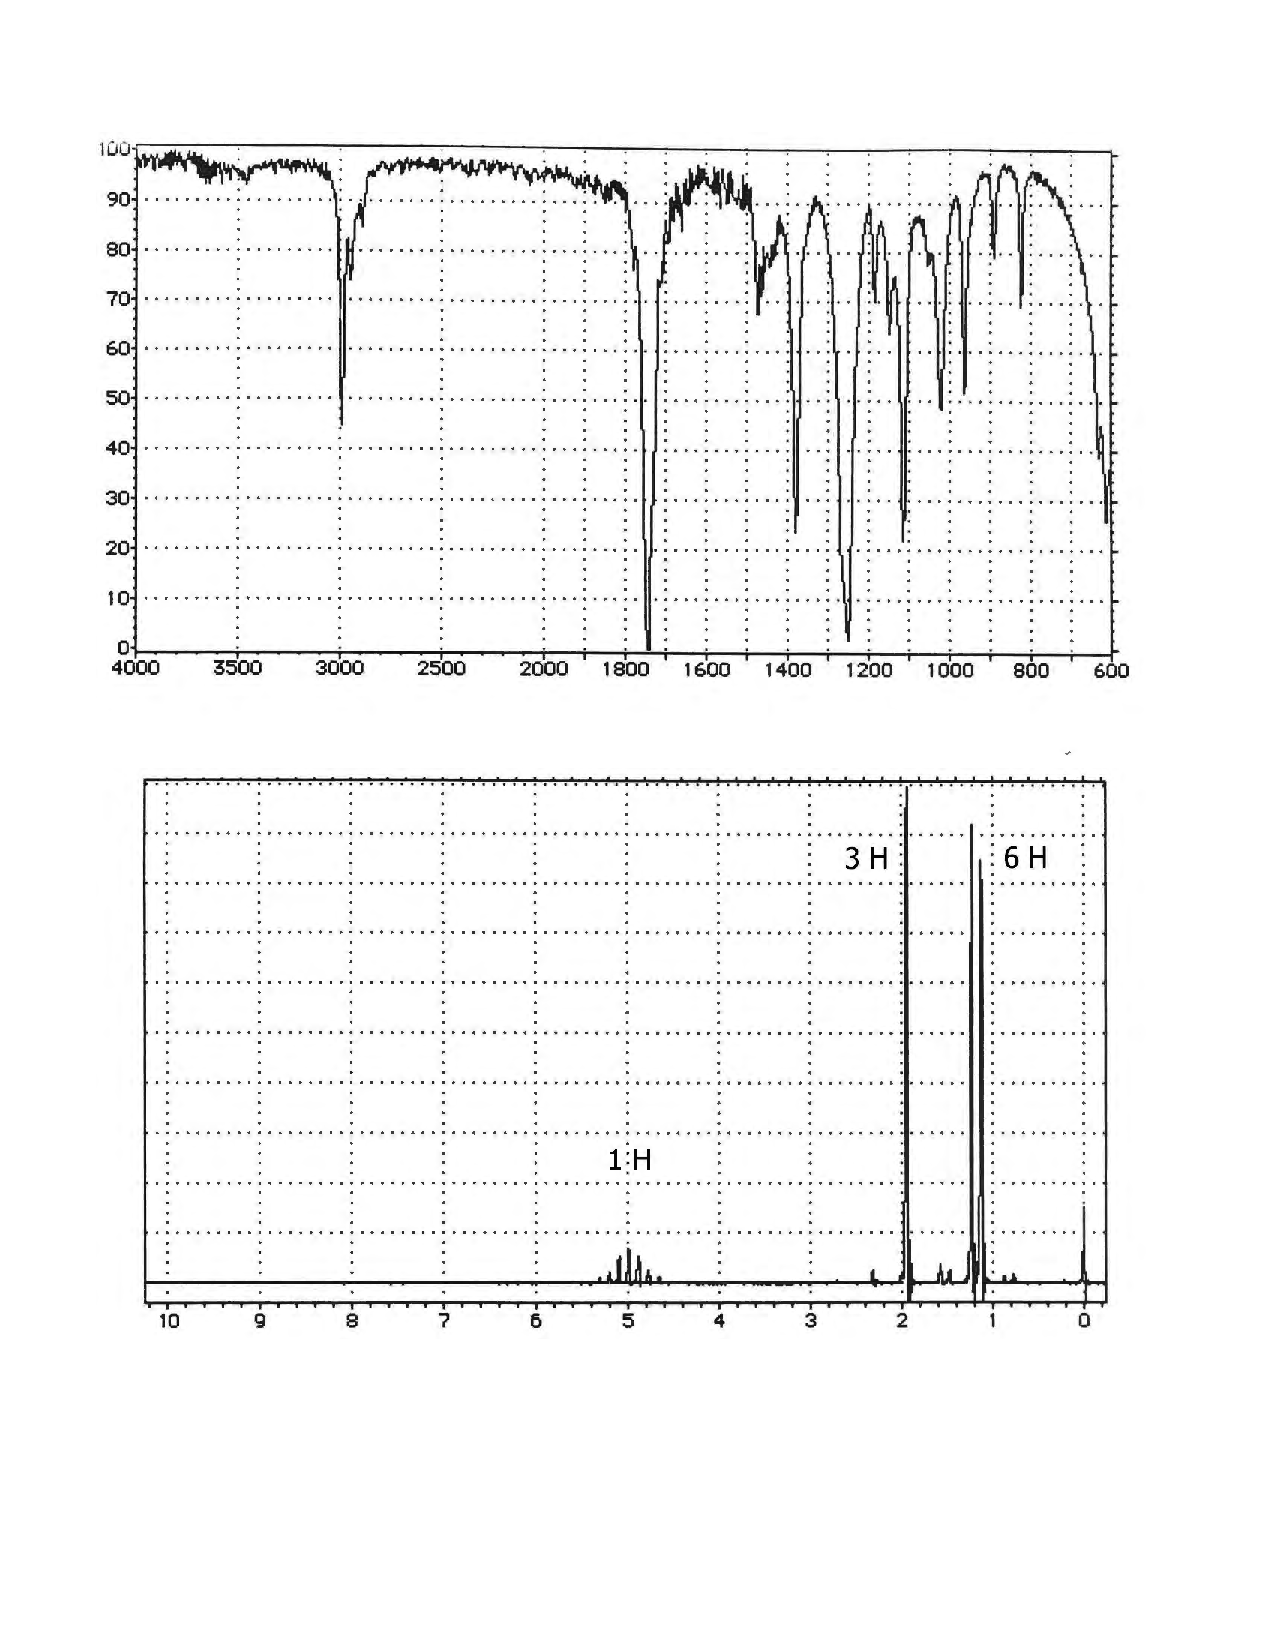
\includegraphics[width=\linewidth]{chimiePC/orga/IR_RMN_5.pdf}

\end{exercise}
\begin{solution}
\begin{center}
    \chemfig{-[1](=[3]O)-[-1]O-[1](-[3])-[-1]}
\end{center}
\end{solution}

\begin{exercise}{Identification IR RMN 6}{1}{PCSI}
{Chimie organique I,Spectroscopie,RMN,Infrarouge}{bermu}

À l'aide des spectres IR et RMN $^{1}$H donnés ci-dessous, ainsi que des tables fournies en annexe, identifier la structure et attribuer les signaux spectroscopiques pertinents de ce composé de formule brute $\mathrm{C_3H_6O_2}$.
 
\vspace{2em}
 
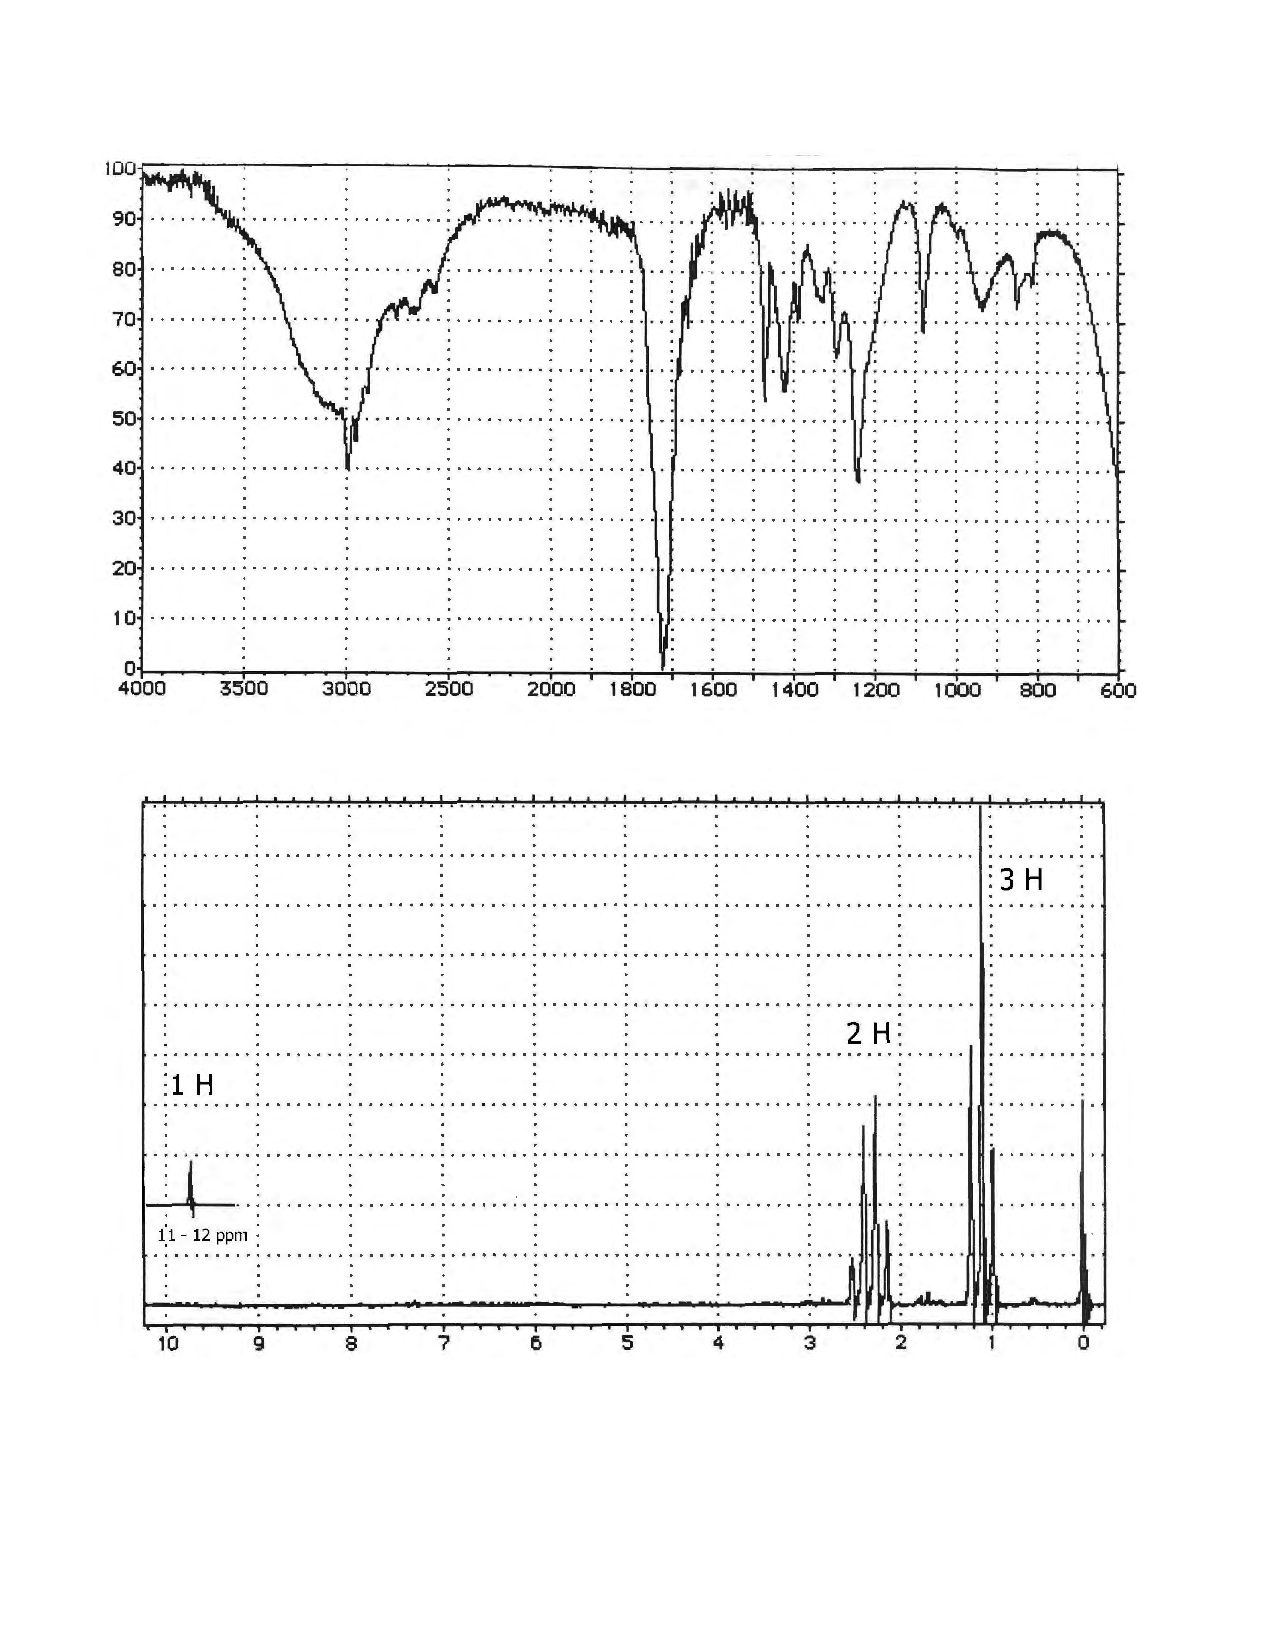
\includegraphics[width=\linewidth]{chimiePC/orga/IR_RMN_6.pdf}

\end{exercise}

\begin{solution}
\begin{center}
    \chemfig{-[-1]-[1](=[3]O)-[-1]OH}
\end{center}
\end{solution}

\begin{exercise}{Identification IR RMN 7}{2}{PCSI}
{Chimie organique I,Spectroscopie,RMN,Infrarouge}{bermu}

À l'aide des spectres IR et RMN $^{1}$H donnés ci-dessous, ainsi que des tables fournies en annexe, identifier la structure et attribuer les signaux spectroscopiques pertinents de ce composé de formule brute $\mathrm{C_9H_{21}N}$.
 
\vspace{2em}
 
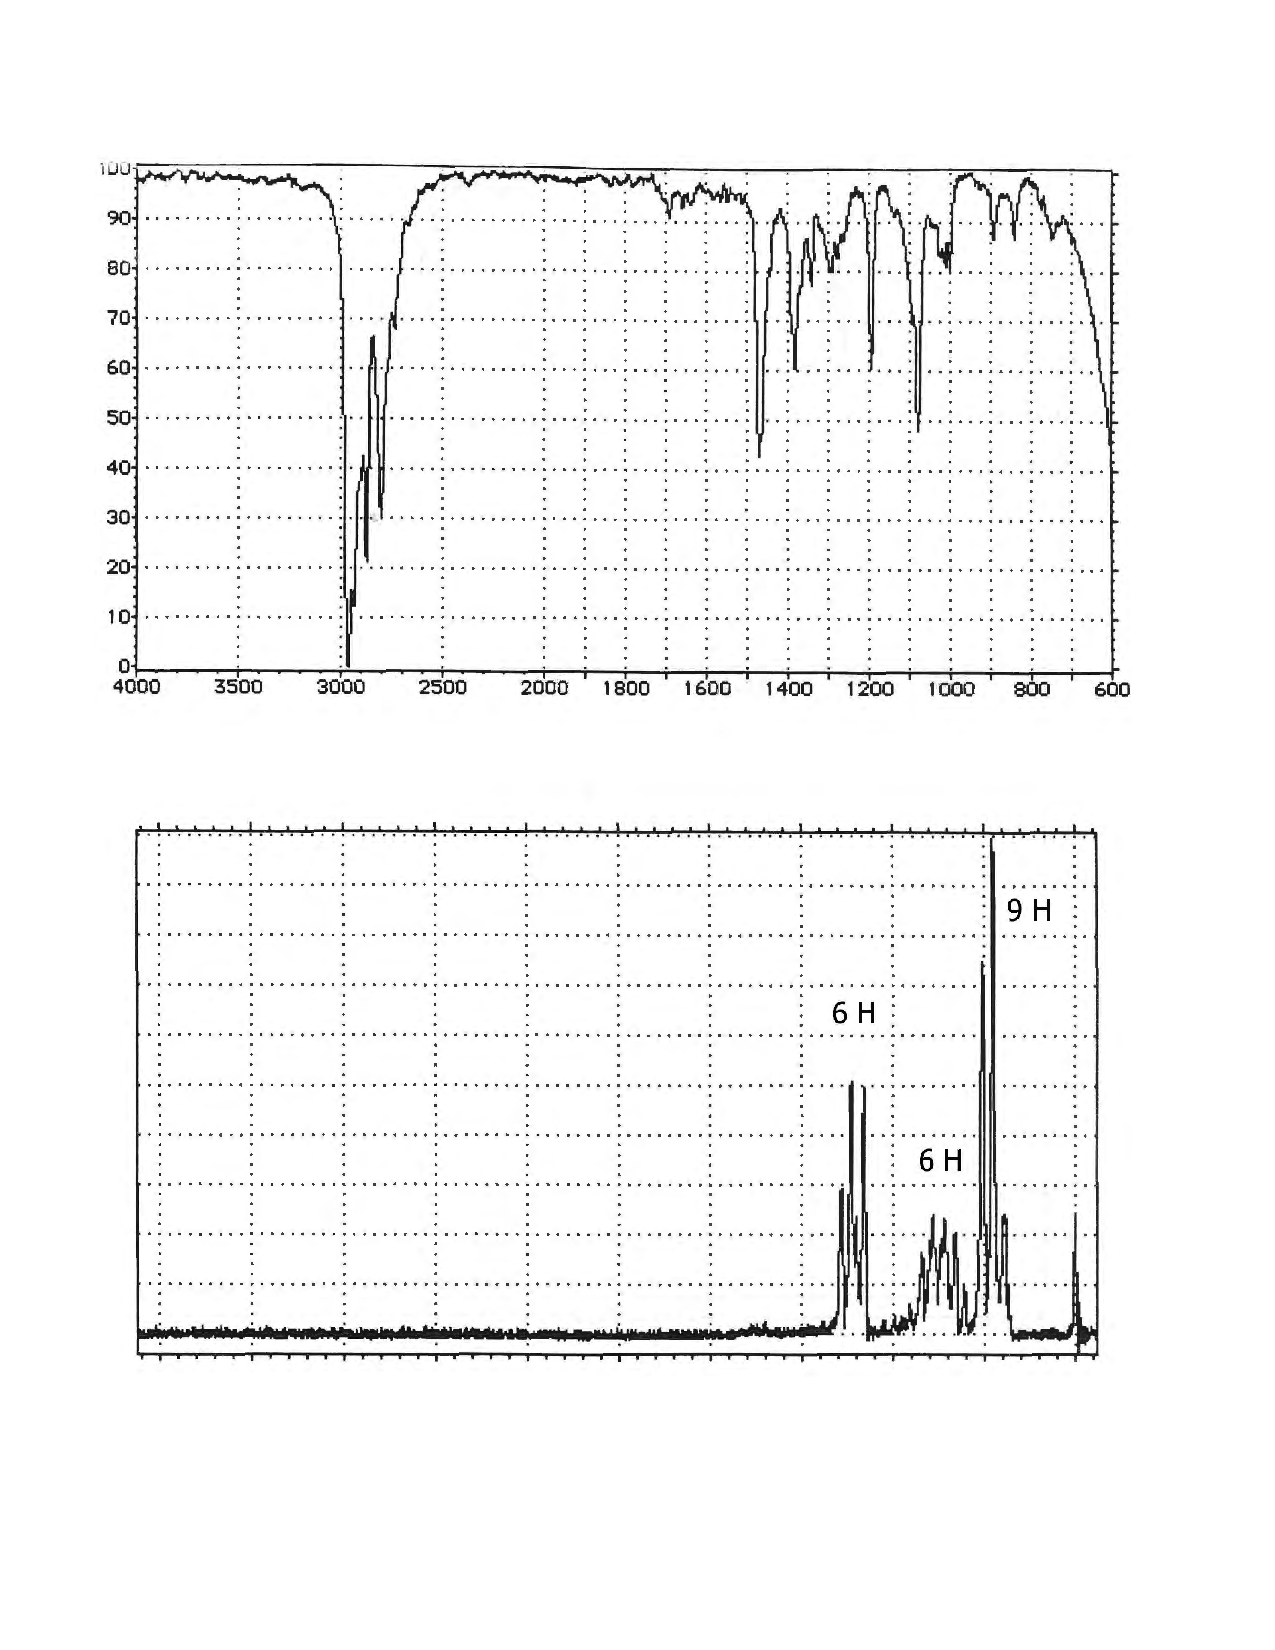
\includegraphics[width=\linewidth]{chimiePC/orga/IR_RMN_7.pdf}

\end{exercise}

\begin{solution}
\begin{center}
    \chemfig{N-[@{left,.5}1]-[-1]-[1]-[@{right,0.75}-1,,,,draw=none]}
    \polymerdelim[height = 5pt, indice = \!3]{left}{right}
\end{center}
\end{solution}

\begin{exercise}{Identification IR RMN 8}{2}{PCSI}
{Chimie organique I,Spectroscopie,RMN,Infrarouge}{bermu}

À l'aide des spectres IR et RMN $^{1}$H donnés ci-dessous, ainsi que des tables fournies en annexe, identifier la structure et attribuer les signaux spectroscopiques pertinents de ce composé de formule brute $\mathrm{C_5H_7NO_2}$.
 
\vspace{2em}
 
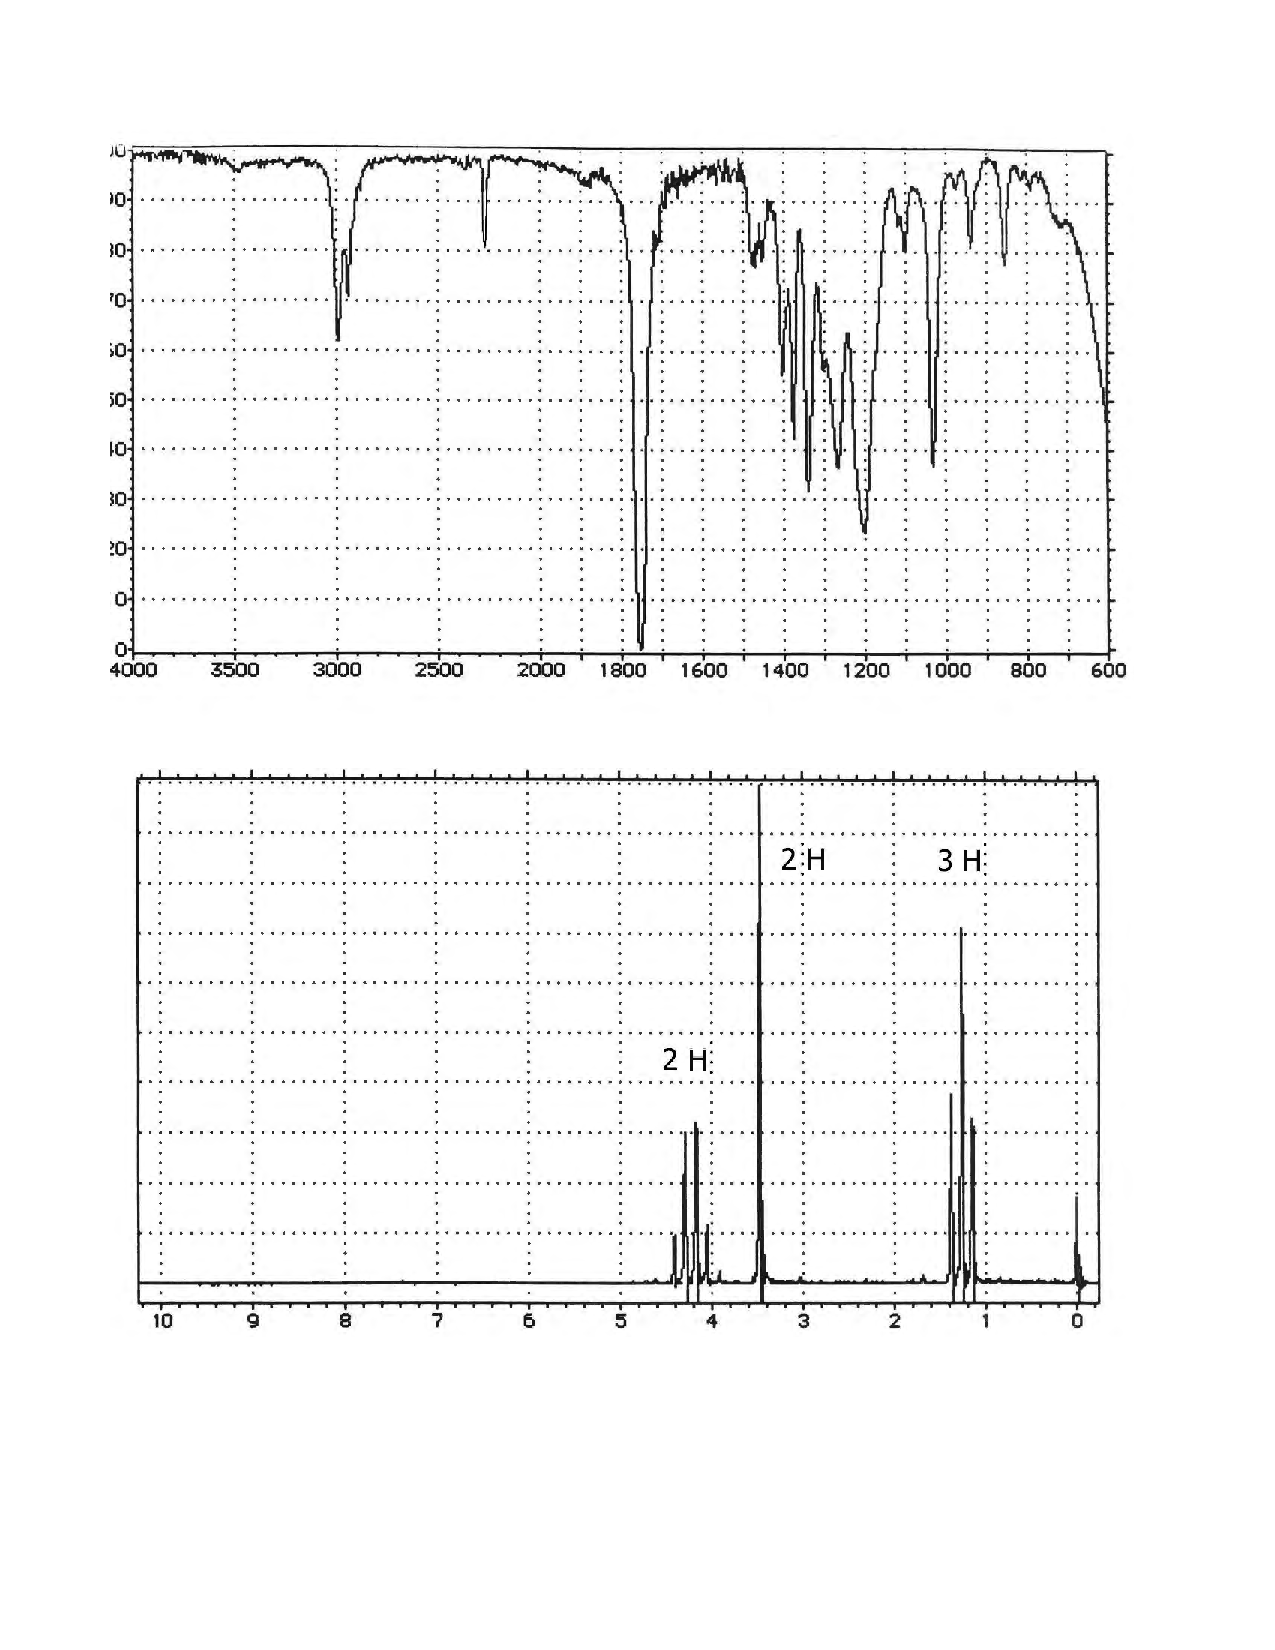
\includegraphics[width=\linewidth]{chimiePC/orga/IR_RMN_8.pdf}

\end{exercise}

\begin{solution}
\begin{center}
    \chemfig{-[-1]-[1](=[3]O)-[-1]O-[1]-[-1]~[-1]N}
\end{center}
\end{solution}

\section{SN/E}
% Niveau :      PCSI *
% Discipline :  Chimie Orga
% Mots clés :  SN, stéréo, cyclohexane

\begin{exercise}{\'Expérience d'Eschenmoser}{3}{PCSI}
{Chimie organique I, SN}{bermu}

\begin{questions}
\questioncours Donnez les mécanismes réactionnels de la $\mathrm{S_N1}$ et de la $\mathrm{S_N2}$ et comparez dans un tableau les différentes propriétés associées (contrôle, sélectivité, nature des réactifs, influence du solvant, de la température, de la concentration ...).

\begin{EnvUplevel}
    En 1970, Albert Eschenmoser réalise une expérience mettant en jeu un réactif $\boldsymbol{\mathrm{(R_H)}}$ et le même réactif avec deux marqueurs deutérés $\mathrm{CD_3}$ $\boldsymbol{\mathrm{(R_D)}}$ en proportion $1:1$,
    \begin{center}
        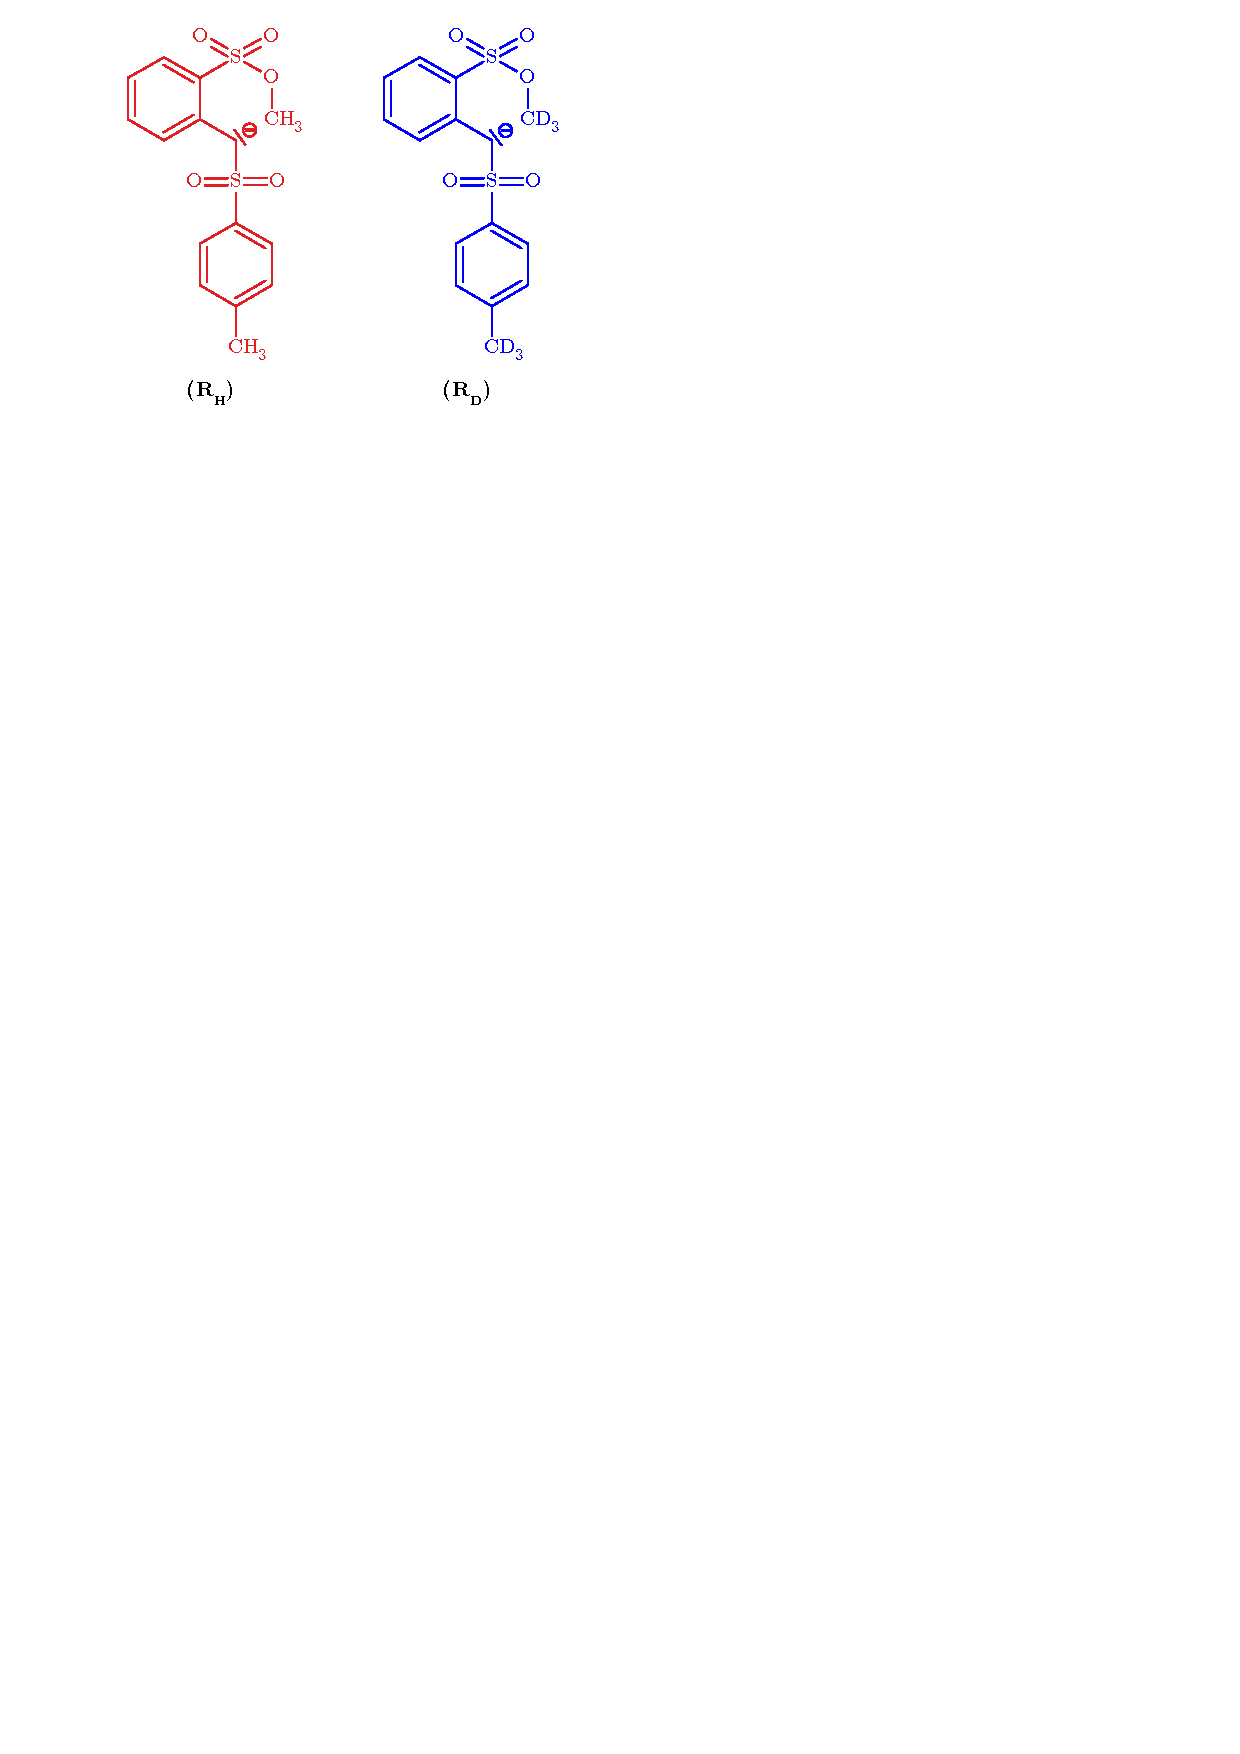
\includegraphics[scale=1.]{chimiePC/orga/eschenmoser.pdf}.
    \end{center}
    Ces molécules réagissent entre elles par substitution nucléophile.
\end{EnvUplevel}
\question Identifiez les groupes nucléophile et nucléofuge de la molécule et en déduire le mécanisme prédominant.

\question Identifiez les 6 réactions possibles et donnez leurs 4 produits formés. \\
On pourra utiliser la notation ---Bs--- (benzènesuflonyle) pour désigner \hspace{-1em} {\footnotesize\chemfig{\text{\color{white}M}-[,.9]*6(=-=(-S(=[3]O)(=[-3]O)-[,.9])-=-=-)}}.

\question \textsf{À l'oral :} Justifiez rapidement l'appellation $\mathrm{S_Ni}$ pour les mécanismes intramoléculaires.

\uplevel{Le résultat de l'expérience d'Eschenmoser est 4 produits trouvés en proportions quasi identiques \mbox{$1:1:1:1$}.}

\question Quelles réactions n'ont pas eu lieu ? Comment qualifier cette sélectivité ?

\uplevel{Nous allons voir pourquoi ces réactions n'ont pas eu lieu. Nous allons tout d'abord nous intéresser aux réactions intramoléculaires.}

\question En supposant que le cycle formé lors du mécanisme concerté est de  même géométrie qu'un cyclohexane en série aliphatique, représentez l'état de transition de la réaction intramoléculaire. \\
On pourra utiliser des notations abrévier les parties superflues des molécules.

\question Conclure quant à la sélectivité observée.

\plusloin A. Eschenmoser \emph{et al.} Endocyclische SN‐Reaktionen am gesättigten Kohlenstoff ?, \textit{Helvetica Chimica Acta}, Vol. 53, No. 8, \textbf{1970},  2059--2069.

\end{questions}
\end{exercise}
% Niveau :      PCSI *
% Discipline :  Chimie Orgam
% Mots clés :   Ballistique, Mécanique du point, PFD, Chute libre

\begin{exercise}{Réactivité du 2-chlorométhylfurane}{2}{PCSI}
{Chimie organique I, SN, SN'{},E}{bermu}

\begin{questions}
\questioncours Aspects cinétiques et thermodynamiques de la concurrence entre les réactions de $\mathrm{S_N1}$, $\mathrm{S_N2}$, et E2. On listera dans un tableau, dans quels cas chaque mécanisme domine.

\begin{EnvUplevel}
    Par la suite, on étudie la réaction du 2-chlorométhylfurane \textbf{A} avec le cyanure de potassium :
    \begin{center}
    \schemestart
        \chemname{\chemfig{[:-18]*5((!\Cnum5)-O(!\Cnum1)-((!\Cnumo{1}2)-[:-24](!\Cnumo{-3}1'{})-[:36]C\ell)=(!\Cnum3)-(!\Cnum4)=(!\Cnum5))}}{\textbf{A}}
        \arrow(.mid east--.mid west){->[KCN][H$_2$O, $40^\circ$C]}[,2]
        \chemname{\chemfig{C_6H_5NO}}{\textbf{B}}
    \schemestop\chemnameinit{}
    \end{center}
\end{EnvUplevel}
\question Proposez une structure pour la molécule \textbf{B}. Quel$\cdot$s mécanisme$\cdot$s peut-on envisager ?

\question Commenter les conditions expérimentales. Quelles précautions faut-il prendre ici ?

\begin{EnvUplevel}
    \vspace{-1.5em}
    \paragraph{Données :} $\mathrm{pK_a}\Big($ \chemfig{N~\chemabove{C}{\scriptstyle\hspace{3.5mm}\ominus}} $\Big/$ \chemfig{N~C-H}$\Big) = 9,2$.
    
    \bigskip
    
    Une étude RMN montre qu'autre produit \textbf{C} est formé en plus de \textbf{B} en proportion 40 : 60. Sur \textbf{C}, le nucléophile s'est substitué sur le C$_5$ de \textbf{A}. Proposer deux mécanismes pour expliquer ce résultat :
\end{EnvUplevel}
    \question l'un s'apparentant à une $\mathrm{S_N1}$, nommé $\mathrm{S_N1}$' ;
    \question l'autre s'apparentant à une $\mathrm{S_N2}$, nommé $\mathrm{S_N2}$'.
    
\uplevel{Il a été montré que la réaction était sous contrôle thermodynamique.}
    \question Expliciter ce que cela signifie et donner, en justifiant, le mécanisme dominant.
    
\begin{EnvUplevel}
    Une étude a été menée cette réaction pour différents substituants sur le carbone 4 de la molécule \textbf{A} :
    \begin{table}[H]
    \centering
    \begin{tabular}{cccc}
        & R$_4$ & \textbf{B} (\%) & \textbf{C} (\%) \\ \hline\hline
       (\textit{i})    &  H    & 40              & 60              \\ \hline
       (\textit{ii})   &  CH(CH$_3$)$_2$     & 16              & 84              \\ 
       (\textit{iii})  &  Br     & 17              & 83             \\  
       (\textit{iv})   &  C(CH$_3$)$_3$     & 25              & 75              \\           
       (\textit{v})   &  CN     & 99              & 1           \\    \hline
    \end{tabular}
    \caption{Proportion des produits \textbf{B} et \textbf{C} formés par la réaction entre \textbf{A} et KCN.}
    \end{table}
\end{EnvUplevel}
    \question Interprétez dans la mesure de vos connaissances ces résultats.
\end{questions}~

\vfill

\plusloin S. Divald \emph{et al.} Reaction of 2,4-chloromethylfurans with Aqueous Potassium Cyanide and Other Nucleophiles, \textit{J. Org. Chem.}, Vol. 41, No. 17, \textbf{1976},  2835--2846.
\end{exercise}
% Niveau :      PCSI *
% Discipline :  Chimie Orgam
% Mots clés :   Ballistique, Mécanique du point, PFD, Chute libre

\begin{exercise}{Réactivité du 2-chlorométhylfurane (II)}{2}{PCSI}
{Chimie organique I, SN, SN'{}}{bermu}

\begin{questions}
\questioncours Aspects cinétiques et thermodynamiques de la concurrence entre les réactions de $\mathrm{S_N1}$, $\mathrm{S_N2}$, et E2. On listera dans un tableau, dans quels cas chaque mécanisme domine.

\begin{EnvUplevel}
    Par la suite, on étudie la réaction suivante :
    
    \begin{center}
    \schemestart
        \chemname{\chemfig{[:-18]*5((!\Cnum5)-O(!\Cnum1)-((!\Cnumo{1}2)-[:-24](!\Cnumo{-3}1'{})-[:36]C\ell)=(!\Cnum3)-(!\Cnum4)=(!\Cnum5))}}{\textbf{A}}
        \+\chemfig{N~\chemabove{C}{\scriptstyle\hspace{3.5mm}\ominus}}\hspace{3.5mm}
        \arrow(.mid east--.mid west)\hspace{3.5mm}
        \chemname{\chemfig{C_6H_5NO}}{\textbf{B}}
        \+\chemfig{\chemabove{C\ell}{\scriptstyle\hspace{5.5mm}\ominus}}
    \schemestop\chemnameinit{}
    \end{center}
\end{EnvUplevel}
\question Proposez une structure pour la molécule \textbf{B}. Quel$\cdot$s mécanisme$\cdot$s peut-on envisager ?

\begin{EnvUplevel}
    \vspace{-2em}
    \paragraph{Données :} $\mathrm{pK_a}\Big($ \chemfig{N~\chemabove{C}{\scriptstyle\hspace{3.5mm}\ominus}} $\Big/$ \chemfig{N~C-H}$\Big) = 9,2$.
    
    \bigskip
    
        Une étude RMN montre qu'autre produit \textbf{C} isomère de \textbf{B} est formé en proportion 40:60.
\end{EnvUplevel}
    
    \question \`A l'aide de la table ci-dessous, donner la structure de \textbf{C}.
  
\begin{EnvUplevel}

\vspace{-2em}
    
\newcolumntype{d}{D{.}{.}{3.2}}

\begin{table}[H]
\centering
\begin{tabular}{rddddddd}
\textbf{OM}                                       & \multicolumn{1}{c}{\textbf{1}} & \multicolumn{1}{c}{\textbf{2}} & \multicolumn{1}{c}{\textbf{3}} & \multicolumn{1}{c}{\textbf{4}} & \multicolumn{1}{c}{\textbf{5}} & \multicolumn{1}{c}{\textbf{6}} & \multicolumn{1}{c}{\textbf{7}} \\
\textbf{\'Energie}                 & \multicolumn{1}{c}{$\alpha + 2,60\beta$}           & 
\multicolumn{1}{c}{$\alpha + 1,78\beta$}           & \multicolumn{1}{c}{$\alpha + 1,39\beta$}           & \multicolumn{1}{c}{$\alpha + 0,88\beta$}           & \multicolumn{1}{c}{$\alpha - 0,15\beta$}           & \multicolumn{1}{c}{$\alpha - 1,17\beta$}           & \multicolumn{1}{c}{$\alpha - 1,75\beta$}           \\ \hline
\multicolumn{1}{r|}{$\mathbf{O_1}$}      & -0,83                          & -0,26                          & -0,42                          & 0,02                           & 0,17                           & 0,20                           & -0,05                          \\
\multicolumn{1}{r|}{$\mathbf{C_2}$}      & -0,35                          & 0,20                           & 0,24                           & -0,54                          & -0,05                          & -0,45                          & 0,53                           \\
\multicolumn{1}{r|}{$\mathbf{C_3}$}      & -0,21                          & 0,13                           & 0,57                           & -0,13                          & 0,52                           & -0,05                          & -0,57                          \\
\multicolumn{1}{r|}{$\mathbf{C_4}$}      & -0,19                          & 0,03                           & 0,55                           & 0,43                           & -0,03                          & 0,50                           & 0,47                           \\
\multicolumn{1}{r|}{$\mathbf{C_5}$}      & -0,28                          & -0,08                          & 0,20                           & 0,50                           & -0,51                          & -0,54                          & -0,25                          \\
\multicolumn{1}{r|}{$\mathbf{C_{1'{}}}$} & -0,16                          & 0,41                           & 0,04                           & -0,36                          & -0,62                          & 0,44                           & -0,32                          \\
\multicolumn{1}{r|}{$\mathbf{C\ell}$}    & -0,09                          & 0,84                           & -0,30                          & 0,37                           & 0,23                           & -0,10                          & 0,06                           \\ \hline
\end{tabular}
\caption{Coefficients des orbitales moléculaires de \textbf{A}.}
\end{table}

\vspace{-1em}

Proposer deux mécanismes pour expliquer ce résultat :
\end{EnvUplevel}  
    \question l'un s'apparentant à une $\mathrm{S_N1}$, nommé $\mathrm{S_N1}$' ;
    \question l'autre s'apparentant à une $\mathrm{S_N2}$, nommé $\mathrm{S_N2}$'.
    
\uplevel{Il a été montré que la température n'avait que peu d'influence sur la proportion \textbf{B}/\textbf{C}.}
    \question Proposer une hypothèse sur les deux mécanismes en concurrence.
    
\begin{EnvUplevel}
    Une étude a été menée cette réaction en variant les substituants aux positions 3 et 4 sur \textbf{A} :
    \begin{table}[H]
    \centering
    \begin{tabular}{ccccc}
        & R$_3$ & R$_4$ & \textbf{B} (\%) & \textbf{C} (\%) \\ \hline\hline
       (\textit{i}) & H     &  H    & 40              & 60              \\
       (\textit{ii}) & H     &  C(CH$_3$)$_3$     & 25              & 75              \\           
       (\textit{iv}) & H     &  CH(CH$_3$)$_2$     & 16              & 84              \\    
       (\textit{v}) & C(CH$_3$)$_3$ & H       & 39              & 61              \\    
       (\textit{vi}) & H     &  Br     & 17              & 83             \\    
       (\textit{vii}) & H     &  CN     & 99              & 1           \\    \hline
    \end{tabular}
    \caption{Proportion des produits \textbf{B} et \textbf{C} formés par la réaction entre \textbf{A} et KCN.}
    \end{table}
    
\vspace{-1em}
\end{EnvUplevel}

    \question Interprétez dans la mesure de vos connaissances ces résultats.
\end{questions}

\plusloin S. Divald \emph{et al.} Reaction of 2,4-chloromethylfurans with Aqueous Potassium Cyanide and Other Nucleophiles, \textit{J. Org. Chem.}, Vol. 41, No. 17, \textbf{1976},  2835--2846.

\end{exercise}

%\begin{center}
%        \chemname{\chemfig{[:-18]**[0,360,dash pattern=on 3pt off 3pt,
%       late options={name=arccenter,label=center:$\oplus$}]5((!\Cnum5)-O(!\Cnum1)-((!\Cnum2)-[:-24,,,,,lddbond](!\Cnum1'{}))-(!\Cnum3)-(!\Cnum4)-(!\Cnum5))}}{\textbf{A'}}
%\end{center}
% Niveau :      PCSI *
% Discipline :  Chimie Orgam
% Mots clés :   Ballistique, Mécanique du point, PFD, Chute libre

\begin{exercise}{\'Elimination de Hofmann}{2}{PCSI}
{Chimie organique I, SN, E}{bermu}

\noindent\textsl{On s'intéresse à la sélectivité de différentes réactions sur le 2-bromo-2-méthylbutane.} \\
\textsl{Pour chaque question, on précisera bien le rôle de chaque composé et des conditions expérimentales.}

\begin{questions}
\questioncours Sélectivité$\cdot$s et spécificité$\cdot$s de la réaction d'élimination sur les halogénoalcanes. On illustrera la question de cours entre autres par les résultats expérimentaux suivants :
\begin{center}
    \schemestart
        \chemfig{-[1]-[-1](-[-3]Br)(<:[2])-[1]}
        \arrow{->[NaOEt][EtOH]}
        \chemname{\chemfig{-[1]=[-1](-[-3])-[1]}}{71\%}
        \arrow{0}[,0]\+\arrow{0}[,0]
        \chemname{\chemfig{-[1]-[-1](-[-3])=[1]}}{29\%}
    \schemestop\chemnameinit{}
    
    \schemestart
        \chemfig{-[1]-[-1](-[-3]Br)(<:[2])-[1]}
        \arrow(.mid east--.mid west){->[NaO$^\textit{t}$Bu][$^\textit{t}$BuOH]}
        \chemname{\chemfig{-[1]=[-1](-[-3])-[1]}}{28\%}
        \arrow{0}[,0]\+\arrow{0}[,0]
        \chemname{\chemfig{-[1]-[-1](-[-3])=[1]}}{72\%}
    \schemestop\chemnameinit{}
    \end{center}
    \noindent--$^\textit{t}$Bu (\emph{tert}-butyle) désigne --$\mathrm{(CH_3)_3}$.
    
    \bigskip

\begin{EnvUplevel}
    Une variante du mécanisme précédent consiste à remplacer le brome par une amine tertiaire à l'aide d'une amidure pour augmenter la sélectivité :
    
    \quad\textbf{\'Etape 1 :}\hspace{2em}\schemestart[][-6]
        \chemfig{-[1]-[-1](-[-3]Br)(<:[2])-[1]}
        \arrow{->[NaNH$_2$][THF, $-70^\circ$C]}[,2.2]
        \textbf{A}
    \schemestop\chemnameinit{}\hspace{1.9em}puis lavage sur Büchner et séchage.
    
    \quad\textbf{\'Etape 2 :}\hspace{1.9em}\schemestart[][base west]
        \textbf{A}
        \arrow{->[MeI (3 eq.)][NaHCO$_3$]}[,1.9]
        \textbf{B}
        \arrow{->[AgOH, H$_2$O][$80^\circ$C]}[,2.1]
        \chemname{\chemfig{-[1]=[-1](-[-3])-[1]}}{5\%}
        \arrow{0}[,0]\+\arrow{0}[,0]
        \chemname{\chemfig{-[1]-[-1](-[-3])=[1]}}{95\%}
    \schemestop\chemnameinit{}
    
    THF (tétrahydrofurane) désigne le solvant \chemfig{[:-198,.7]*5(-O----)}\,.
\end{EnvUplevel}
    \question Quelle est la nature de la première étape ? Donner la structure de \textbf{A}. \\
        Justifier le choix de température et de solvant.
    \question Quelle est la nature de la réaction \textbf{A} $\longrightarrow$ \textbf{B} ? Donner la structure de \textbf{B}.
    \question Préciser le rôle de NaHCO$_3$. Quel est l'intérêt de NaHCO$_3$ en particulier ?
    \question Que se passe-t-il lors de la dernière étape ?  Interpréter la sélectivité finale.
    \question Discuter du choix de $\mathrm{I}^\ominus$ et $\mathrm{Ag}^\oplus$.
    
    \question Conclure quant à l'effet des chaînes carbonées sur la sélectivité des réactions des questions précédentes.
\end{questions}

\vfill

\plusloin A. W. von Hofmann,Beiträge zur Kenntniss der flüchtigen organischen Basen, \textit{Annalen der Chemie und Pharmacie}, Vol. 78, No. 3, \textbf{1851},  253--286.

\end{exercise}

\begin{solution}
\begin{center}\small\schemestart
        \chemfig{-[1]-[-1](-[-3]Br)(<:[2])-[1]}
        \arrow{->[NaNH$_2$]}
        \chemname{\chemfig{-[1]-[-1](-[-3]NH_2)(<[2])-[1]}}{\textbf{A}}
        \arrow{->[MeI]}
        \chemname{\chemfig{-[1]-[-1](-[-3]\chemabove{N}{\scriptstyle\hspace{3.5mm}\oplus}(-[0,1.4]\chemabove{\ ,\ I}{\scriptstyle\hspace{5.5mm}\ominus})(-[-3])-[6])(<[2])-[1]}}{\textbf{B}}
        \arrow{->[AgOH]}
        ...
    \schemestop\chemnameinit{}\end{center}
\end{solution}
% Niveau :      PCSI *
% Discipline :  Chimie Orgam
% Mots clés :   Ballistique, Mécanique du point, PFD, Chute libre

\begin{exercise}{Réactivité du chlorure de menthyle}{2}{PCSI}
{Chimie organique I, SN, E}{poublanc,bermu}

\begin{questions}
\questioncours Activation nucléophile des alcools : principe et intérêt synthétique.
%Sélectivité$\cdot$s et spécificité$\cdot$s de la réaction d'élimination sur les halogénoalcanes.

\begin{EnvUplevel}
    On s'intéresse à présent à la réactivité du chlorure de menthyle \textbf{A} et du chlorure de néomenthyle \textbf{B}.
    
        ~\hfill
        \chemfig{>:[-3]*6(---(-[-3,,,,Cram2Sides](-[7])(-[-3,1.2,,,draw=none]{\textbf{A}})-[-1])-(<:[-1,1.2]C\ell)--)}
        \hfill
        \chemfig{>:[-3]*6(---(-[-3,,,,Cram2Sides](-[7])(-[-3,1.2,,,draw=none]{\textbf{B}})-[-1])-(<[-1,1.2]C\ell)--)}
        \hfill~
\end{EnvUplevel}
    \question Quelle est la relation de stéréochimique entre ces deux isomères ?

\begin{EnvUplevel}
    Lors de la réaction de \textbf{A} et \textbf{B} avec l'éthanolate de sodium, on observe la formation de deux produits :
    
    ~\hfill\schemestart[][west]
        \textbf{A}, \textbf{B}
        \arrow{->[NaOEt][EtOH, $70^\circ$C]}[,2.1]
        \textbf{C} + \textbf{D},
    \schemestop\chemnameinit{}\hfill (R\arabic{exercise})
    
    \textbf{C} étant le produit ayant un stéréodescripteur RS, et \textbf{D} celui ayant un stéréodescripteur S.
\end{EnvUplevel}
    \question Quelle est la nature de la réaction précédente ? Donner la structure des produits formés.
    \question Commenter les conditions expérimentales.
\begin{EnvUplevel}
On observe que la vitesse de réaction et la proportion \textbf{C} : \textbf{D} varie selon que le substrat soit \textbf{A} ou \textbf{B}.
\begin{table}[H]
    \centering
    \begin{tabular}{rccc}
        Substrat & $k$ (rel.) & \textbf{C} (\%) & \textbf{D} (\%) \\ \hline\hline
        \textbf{A} & $10^{-2}$ & 99,9 & 0,01 \\
        \textbf{B} & $10^{0}$  & 25,4 & 74,6 \\ \hline
    \end{tabular}
    \caption{Constante de vitesse et proportion des produits obtenus lors de la réaction (R\arabic{exercise}).}
\end{table}
\end{EnvUplevel}
    \question Qualifier ce constat expérimental.
    \question Interpréter ces faits expérimentaux et écrire le mécanisme de la réaction dans chaque cas.
    \paragraph{Aide :} représenter \textbf{A} et \textbf{B} dans leur conformation la plus stable.\vspace{1.5em}
\end{questions}

\end{exercise}

    

\section{AN/Organomet}
% Niveau :      PCSI *
% Discipline :  Chimie Orgam
% Mots clés :   Ballistique, Mécanique du point, PFD, Chute libre

\begin{exercise}{Régiosélectivité des organométalliques}{2}{PCSI}
{Chimie organique I, AN, organométallique}{bermu}

\begin{questions}
\questioncours Structure et propriétés chimiques des organomagnésiens mixtes.

\begin{EnvUplevel}
On étudie la réaction de différents composés organométalliques sur la pent-3-èn-2-one \textbf{A} :
\begin{center}
    \schemestart
        \textbf{A}
        \arrow(--[xshift=-3.5em]){->[MeMgBr][Et$_2$O, reflux]}[,2.1]
        \mbox{}%
        \arrow{->[H$^+$][H$_2$O, $0^\circ$C]}[,1.9]
        \chemname{\chemfig{C_6H_{12}O}}{\textbf{B}}
    \schemestop\chemnameinit{}
    \end{center}
\end{EnvUplevel}

\question Donner la structure de \textbf{B} et le mécanisme de la réaction. \\
On précisera la structure de l'intermédiaire réactionnel formé avant l'hydrolyse finale ?

\question Commenter les conditions expérimentales. Quelles précautions expérimentales faut-il prendre lors de cette synthèse ?

\question Donner rapidement le mode de formation de MeMgBr.

\question Quel sont les deux effets de l'hydrolyse finale ?

\uplevel{Lors de cette réaction, on observe la présence d'un produit supplémentaire \textbf{C} isomère de chaîne de \textbf{B}.}

\question Identifier le second site électrophile de \textbf{A} et donner la structure de \textbf{C}.

\question Donner le mécanisme de la première étape de la formation de \textbf{C}.

\begin{EnvUplevel}
Il exsite d'autres composés organometalliques qui ont un comportement analogue à celui des organomagnésiens dont les propriétés varient en fonction du métal M employé lors de la réaction. Ainsi, lors de la réaction précédente, la proportion \textbf{B} : \textbf{C} varie comme l'indique la table ci-dessous.

\begin{table}[H]
    \centering
    \begin{tabular}{rlccr}
        Organométallique & CH$_3$--M & \'Electroneg.$^\ast$ & \% ion. C--M & \textbf{B} : \textbf{C} \\ \hline\hline
        Organopotassique      & CH$_3$--K    & 0,82 & 53 & $\sim 1:0$~ \\
        Organosodique         & CH$_3$--Na   & 0,93 & 48 & $99:1$~ \\
        Organolithien         & CH$_3$--Li   & 0,98 & 46 & $98:2$~ \\
        Organomagnésien mixte & CH$_3$--MgBr & 1,55 & 32 & $86:14$ \\
        Organozincique mixte  & CH$_3$--ZnBr & 1,65 & 32 & $72:28$ \\
        Organocuprate lithié  & CH$_3$--CuLi & 1,90 & 10 & $\sim 0:1$~ \\ \hline
    \end{tabular}
    \begin{flushleft}
        \small $^\ast$ \'Electronégativité de M au sens de Pauling, à comparer avec celle du carbone : 2,55.
    \end{flushleft}
    \caption{Propriétés et sélectivité de différents composés organométalliques.}
\end{table}
\end{EnvUplevel}

\question Interpréter à l'aide des données ci-dessus l'évolution du caractère ionique de la liaison carbone--métal (C--M) des différents composés organométalliques.

\question Commenter la sélectivité de ces composés. Les organomagnésiens sont-ils sélectifs ?


\end{questions}
\end{exercise}
% Niveau :      PCSI *
% Discipline :  Chimie Orgam
% Mots clés :   Ballistique, Mécanique du point, PFD, Chute libre

\begin{exercise}{Synthèse de Bouveault}{2}{PCSI}
{Chimie organique I, AN,  organométallique}{bermu}
\index{AN+E}\index{amide}

\begin{questions}
\questioncours Réactivité et intérêt synthétique des organomagnésiens mixtes.

\begin{EnvUplevel}
Parmi les autres intérêts sythétiques des organomagnésiens, le chimiste français Louis Bouveault a trouvé en 1904 une voie de synthèse originale utilisant les organomagnésiens.

Partant du chlorure d'éthyle \textbf{A},
\begin{center}
    \schemestart
        \textbf{A}
        \arrow{->[Mg$^0$][DMF, reflux]}[,2.1]
        \textbf{B}
        \arrow{->[DMF][reflux]}[,1.5]
        \textbf{C}
        \arrow{->[H$^+$][H$_2$O, $0^\circ$C]}[,1.9]
        \textbf{D}
        %\chemname{\chemfig{C_3H_6O}}{\textbf{D}}
    \schemestop\chemnameinit{}~,
    \end{center}
on forme le composé \textbf{D}. DMF désigne ici le N,N-diméthylformamide : \chemfig{H-[1,.7](=[3,.7]O)-[-1,.7]N(-[-3,.7])-[1,.7]}\,.
\end{EnvUplevel}

\question Donner la structure et préciser le protocole expérimental de formation de \textbf{B}.

\question Donner la structure de l'intermédiaire \textbf{C} et le mécanisme de sa formation.

\begin{EnvUplevel}
L'espèce \textbf{C} est ensuite hydrolysée à basse température. Après lavage et séchage, l'espèce \textbf{D} est caractérisée par spectroscopie infrarouge. On donne ci-dessous les spectres des produits et des réactifs de la synthèse. \vspace{-1em}
\begin{figure}[H]
    \centering
    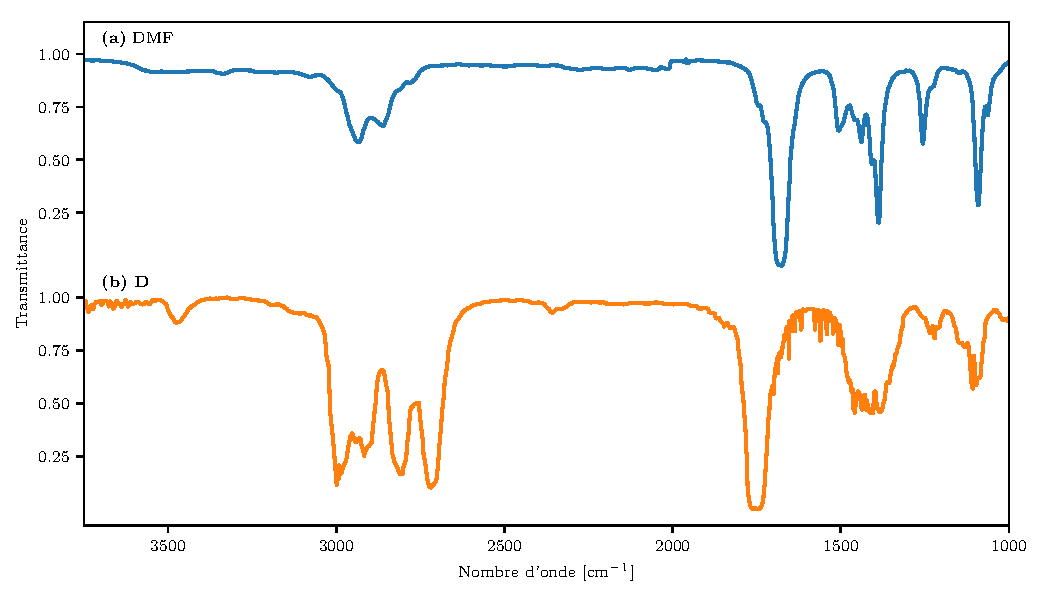
\includegraphics[width=\linewidth]{chimiePC/orga/bouveault.pdf}\vspace{-.5em}
    \caption{Spectres infrarouges du DMF \textbf{(a)} et du produit final obtenu \textbf{D (b)}.}
\end{figure}
\end{EnvUplevel}

\question Justifier les conditions expérimentales de la dernière étape.

\question Identifier sur les spectres IR ci-dessus les fonctions créées et détruites lors de la synthèse. \\
Vous pouvez vous aider si besoin d'une table IR.

\question Donner la structure de \textbf{D} et justifier le caractère nucléofuge du groupe partant lors de \textbf{C} $\longrightarrow$ \textbf{D}.

\question Proposer succinctement un protocole pour isoler \textbf{D}.

\question Proposer d'éventuels sous-produits de ce protocole expérimental.

\question Quel est l'intérêt de cette synthèse ?


\end{questions}
\end{exercise}

\begin{solution}
\begin{questions}
    \questioncours R--Mg--X est un excellent nucléophile, une excellente base (au sens de Lewis et de Brönsted) et un bon réducteur.
    
    Le carbone de R--Mg--X est chargé $\delta^-$, ce qui est très utile en chimie organique pour assembler différents édifices carbonés : moyen de créer des liasons C--C.
    
    Permet aussi de former des alcools par réaction sur les carbonylés.
    
    \question \textbf{B} : $\mathrm{CH_3}$--Mg--Br, cf{.} cours pour le protocole.
    
    \question\hfill
    \schemestart
        \chemname{\chemfig{CH_3-[@{a1},1.5,,,red]MgBr}}{\textbf{B}}
        \+
        \chemname{\chemfig{H-[1]@{b1}(=[@{a2}3]@{b2}\lewis{13,O})-[-1]\lewis{2,N}(-[-3])-[1]}}{DMF}
        \chemmove[red,-stealth,red,shorten >=3pt]{
            \draw(a1)..controls +(up:10mm) and +(north west:10mm).. (b1);}
        \chemmove[red,-stealth,red,shorten <=2pt]{
            \draw(a2)..controls +(west:2mm) and +(south west:5mm).. (b2);}
        \arrow{->}
        \chemname{\chemfig{H-[1](-[4])(-[2]O^\ominus,\:MgBr^\oplus)-[-1]\lewis{2,N}(-[-3])-[1]}}{\textbf{C}}
    \schemestop\chemnameinit{}\hfill~
    
    \question Lors de \textbf{C} $\longrightarrow$ \textbf{D}, l'eau sert à hydrolyser \textbf{C} mais aussi à détruire l'excédent de \textbf{B} et de magnésium. La réaction est très exothermique ($\Delta$pK$_a \simeq$ 20), et donc il faut la faire à basse température par précaution.
    
    \question \`A la fin de cette étape, il y a une phase organique chargée en \textbf{D} avec quelques polluants ioniques et une phase aqueuse chargée de sous-produits.
    
    On peut laver et décanter la phase organique puis évaporer le gros du solvant à l'évaporateur rotatif. Enfin, on peut isoler \textbf{D} par distillation fractionnée.
    
    \question Il n'y a pas de bande large O--H à 3500 cm$^{-1}$ comme on s'y attendrait : on ne forme donc pas un alcool. La bande C$=$O à 1700 cm$^{-1}$ se décale suggérant que l'on passe d'une amide à un carbonyle (cétone ou aldéhyde). Le pic C--N à 1150 cm$^{-1}$ disparaît.
     
    \question Penser à l'analogie entre les esters et les amides. Suggestion de mécanisme concerté (on peut l'envisager aussi en plusieurs étapes) :
    \begin{center}\schemestart
        \chemname{\chemfig{H-[1](-[4])(-[2]O^\ominus,\:MgBr^\oplus)-[-1]\lewis{2,N}(-[-3])-[1]}}{\textbf{C}}
        \arrow{->[H$^+$][$-$ MgBr$^\oplus$]}[,1.9]
        \chemname{\chemfig{H-[1](-[4])(-[@{b1}2]\lewis{23,O}-[@{a1},,,,red]@{b2}H)-[@{a2}-1,,,,red]\lewis{2,N}(-[-3])-[1]}}{\textbf{C'}}
        \chemmove[red,-stealth,red,shorten >=3pt]{
            \draw(a1)..controls +(south:5mm) and +(south east:3mm).. (b1);
            \draw(a2)..controls +(north east:4mm) and +(down:7mm).. (b2);}
        \arrow{->[][$-$ HN(CH$_3$)$_2$]}[,2.1]
        \chemname{\chemfig{-[1](=[3]O)-[-1]H}}{\textbf{D}}
    \schemestop\chemnameinit{}
    \end{center}
    
    L'amine HN(CH$_3$)$_2$ est un très bon nucléofuge car elle est une base de Lewis encombrée.
    
    \question L'amine HN(CH$_3$)$_2$ est rejetée à la suite de la seconde étape, on peut la faire passer en solution en diminuant le pH : $\mathrm{HN(CH_3)_2 + H^+ \longrightarrow H_2N^+(CH_3)_2}$. On pourrait également envisager la présence comme sous-produit de \textbf{C'}, intermédiaire pour lequel il n'y a pas eu de départ nucléofuge.
    
    \question Cette synthèse permet donc de synthétiser des aldéhydes avec des organomagnésiens ce qui est normalement compliqué car les aldéhydes sont attaqués par les organomagnésiens.
    
\end{questions}
\end{solution}
% Niveau :      PCSI *
% Discipline :  Chimie Orgam
% Mots clés :   Ballistique, Mécanique du point, PFD, Chute libre

\begin{exercise}{Réaction de Meerwein--Ponndorf--Verley}{3}{PCSI}
{Chimie organique I, AN, SN, E, acétalisation, organométallique}{bermu}

\begin{questions}
\questioncours Préparation expérimentale du bromure de 2-méthylpropylmagnésium \textbf{A}. \\
On détaillera précisément le protocole expérimental avec schémas ainsi que les précautions à prendre et les réactions parasites.

\begin{EnvUplevel}
On se propose d'étudier la séquence réactionnelle qui, partant de la 4,4-diméthylpentan-2-one \textbf{B}
\begin{center}
    \schemestart
        \textbf{B}
        \arrow{->[\textbf{A}][Et$_2$O, reflux]}[,2.1]
        \textbf{C $+$ D}
        \arrow{->[H$^+$][H$_2$O, $0^\circ$C]}[,1.9]
        \textbf{E $+$ D}
    \schemestop\chemnameinit{}~,
    \end{center}
forme l'alcène \textbf{D} ($\mathrm{C_4H_8}$) et l'alcool \textbf{E} ($\mathrm{C_7H_{15}OH}$).
\end{EnvUplevel}

\question Donner la structure de \textbf{C} ainsi que son mécanisme de formation.

\question Déduire la structure de \textbf{E} et commenter les conditions expérimentales de la réaction \textbf{D} $\longrightarrow$ \textbf{E}.

\question Quelles structures sont possibles pour \textbf{D} ? Laquelle vous parait la plus cohérente ?

\uplevel{Zimmerman et Traxler ont proposé d'interpréter la formation de \textbf{D} par un état de transition \textbf{AB} \\ (\textbf{A} + \textbf{B}) ayant une géométrie de cycle cyclohexanique.}

\question En représentant en pointillés les liaisons créées et détruites entre \textbf{A} et \textbf{B}, donner la structure de \textbf{AB}.

\question En déduire le mécanisme concerté \textbf{A} + \textbf{B} $\longrightarrow$ \textbf{C} + \textbf{D}.

\uplevel{Mosher en 1950 a montré que la réaction était énantiosélective en effectuant la séquence réactionnelle précédente en remplacant \textbf{A} par \\
\chemfig{-[1](-[3]Et)-[-1]-[1]MgBr}.}

\question Interpréter ce résultat.


\end{questions}
\end{exercise}
% Niveau :      PCSI *
% Discipline :  Chimie Orgam
% Mots clés :   Ballistique, Mécanique du point, PFD, Chute libre

\begin{exercise}{Brèves : rétrosynthèse}{2}{PCSI}
{Chimie organique I, AN, SN, E, acétalisation, organométallique}{bermu}

Proposer un schéma de synthèse pour les espèces suivantes : \\[1em]

\begin{tabular}{cc}
    \chemfig{*6(---(-(-[3]OH)-[-1]*6(------))---)} & \chemfig{-[1](-[3])-[-1]-[1]-[-1](-[-4])(-[-2]OH)-[1]-[-1]-[1](-[3])-[-1]} \\
    \textsfbf{A} & \textsfbf{B}
\end{tabular}

\end{exercise}

\section{Activation de groupes caractéristiques}
% Niveau :      PCSI *
% Discipline :  Chimie Orgam
% Mots clés :   Ballistique, Mécanique du point, PFD, Chute libre

\begin{exercise}{Réarrangement de Wagner--Meerwein}{3}{PCSI}
{Chimie organique I, SN, E, Réarrangement, Activation}{bermu}

\begin{questions}
\questioncours Intérêt synthétiques et méthodes d'activation électrophile des alcools.

\begin{EnvUplevel}
    L'activation électrophile des alcools en milieu acide peut être suivie d'un mécanisme de d'élimination monomoléculaire E1 en deux étapes :
    \begin{itemize}
        \item la première analogue à celle d'une $\mathrm{S_N1}$,
        \item la seconde analogue à une E2.
    \end{itemize}
\end{EnvUplevel}

\question \`A l'aide de vos connaissances et de la question précédente proposer un mécanisme d'une E1 sur le 2-méthylpropan-2-ol dans la l'acide sulfurique concentré. \\
On pretera bien attention au fait qu'on se trouve en milieu acide.

\question Quel est le critère cinétique ou thermodynamique qui détermine si une E1 se fait spontanément ?

\begin{EnvUplevel}
    On s'intéresse à présent à la réaction des alcools dérivés du bornane
    \begin{center}
        \chemfig{?[a](!\Cnumo{6}2)-[:10]?[b,1,over line](!\Cnumo{-3}1)(-[:-140](!\Cnumo{:-140}1'{}))-[:-10](!\Cnumo{0}6)-[:50](!\Cnum5)-[:170](!\Cnumo{1}4)(-[:120,1.1]?[b](!\Cnumo{3}7)(-[1](!\Cnum7''{}))-[5](!\Cnumo{6}7'{}))-[:-170,.55]-[:-170,.2,,,draw=none]-[:-170,.25]?[a](!\Cnumo{6}3)}
    \end{center}
    dans l'acide sulfurique concentré.
\end{EnvUplevel}

%\question Combien y a-t-il de monoalcools dérivés du bornane (en prenannt en compte les stéréoisomères) ? Ne pas les représenter.

\question Justifier les résultats expérimentaux suivants :
\begin{parts}
    \part L'alcool substitué sur le carbone 4 ne réagit pas du tout.
    \part Les alcools substitués sur les carbones 1', 7' et 7'' réagissent peu.
\end{parts}

\question Quel est le produit formé par la réaction de l'alcool substitué sur le carbone 2 (ou 6) ?

\begin{EnvUplevel}
Le produit formé par cette réaction est en fait le camphène :
    \begin{center}
        \chemfig{?[a]-[:10]?[b,1,over line]-[:-10](=[-2])-[:50](-[-3])(-[:10])-[:170](-[:120,1.1]?[b])-[:-170,.55]-[:-170,.2,,,draw=none]-[:-170,.25]?[a]}
    \end{center}
\end{EnvUplevel}
    \question Proposez un mécanisme pour expliquer cette réaction.\\
    Justifiez la nomenclature de réarrangement 1,2 pour cette réaction.
\end{questions}

\end{exercise}

\begin{solution}
\begin{questions}
\questioncours Les alcools ne sont pas de bons nucléofuges. Pour les transformer en bon groupe partants (activation électrophile), on peut :
    \begin{itemize}
        \item ajouter un H$^+$ dans un acide fort : R-OH + H$^+$ = R-H$_2$O$^+$
        \item remplacer le OH par un OR très encombré, par exemple avec des sulfonyles (tosylate, mésylate), qui ont l'avantage d'être des bases faibles et des mauvais nucléophiles.
    \end{itemize}

\question En milieu acide, il y a tout d'abord une activation électrophile du brome (Q1) : \\[1ex]

\hfill\schemestart
        \chemfig{-[1](-[:-109])(-[-1])-[3]@{br}\lewis{024,Br}}
        \arrow{->[\chemfig{@{h}\lewis{4|,H}^\oplus}][]}
        \chemfig{-[1](-[:-109])(-[-1])-[3]\lewis{24,Br}^\oplus-[0,1.3]H}
        \chemmove[red,-stealth,red,shorten <= 2pt, shorten >= 4pt]{
            \draw(br)..controls +(up:10mm) and +(west:10mm).. (h);}
\schemestop\hfill~

Puis la E1 :\hfill\schemestart
        \chemfig{-[1](-[:-109])(-[-1])-[@{a1}3,,,,red]@{b1}\lewis{24,Br}^\oplus-[0,1.3]H}
        \arrow{->[][$-$ HBr]}
        \chemfig{-[2](-[6,0.2,,,draw=none]@{b2}\chemabove{\lewis{4|,}}{\quad\scriptsize\oplus})(-[4])-[0]-[@{a2}-2,,,,red]H}
        \chemmove[red,-stealth,red,shorten >= 5pt]{
            \draw(a1)..controls +(west:3mm) and +(south west:3mm).. (b1);
            \draw(a2)..controls +(west:3mm) and +(south east:3mm).. (b2);}
        \arrow{->}
        \chemfig{-[2](-[4])=[0]}
    \schemestop\chemnameinit{}\hfill~

\question ~
\begin{parts}
    \part La formation du carbocation en C$_4$ est impossible à cause des contraintes angulaires cycle.
    \part Les carbocations 1' et 7' sont peu stables car primaires.
\end{parts}

\question Si on suit le mécanisme précédent on obtient la structure (peu stable) suivante

\hfill\schemestart
        \chemfig{?[a](-[:170]@{oh}O-[6,.4,,,draw=none]H)-[:10]?[b,1,over line](-[:-140])-[:-10]-[:50]-[:170](-[:120,1.1]?[b](-[1])-[5])-[:-170,.55]-[:-170,.2,,,draw=none]-[:-170,.25]?[a]}
        \arrow{->[\chemfig{@{h}\lewis{4|,H}^\oplus}][]}
        \chemmove[red,-stealth,red,shorten <= 2pt, shorten >= 4pt]{
            \draw(oh)..controls +(south east:20mm) and +(west:10mm).. (h);}
        \chemfig{?[a](-[6,0.2,,,draw=none]@{b1}\chemabove{\lewis{4|,}}{\quad\scriptsize\oplus})-[:10]?[b,1,over line](-[:-140])-[:-10]-[:50]-[:170](-[:120,1.1]?[b](-[1])-[5])-[:-170,.55]-[:-170,.2,,,draw=none]-[:-170,.25]?[a]-[@{a1}:170,,,,red]H}
        \chemmove[red,-stealth,red,shorten >= 3pt]{
            \draw(a1)..controls +(south west:2mm) and +(west:2mm).. (b1);}
        \arrow{->[][$-$ H$^\oplus$]}
        \chemfig{(=[:50]?[a])-[:10]?[b,1,over line](-[:-140])-[:-10]-[:50]-[:170](-[:120,1.1]?[b](-[1])-[5])-[:-170,.55]-[:-170,.2,,,draw=none]?[a]}
\schemestop\hfill~

    \question Il y a une délocatisation électronique (ce qu'on appelle un réarrangement) :
    
\hfill\schemestart
        \chemfig{?[a](-[:170]@{oh}O-[6,.4,,,draw=none]H)-[:10]?[b,1,over line](-[:-140])-[:-10]-[:50]-[:170](-[:120,1.1]?[b](-[1])-[5])-[:-170,.55]-[:-170,.2,,,draw=none]-[:-170,.25]?[a]}
        \arrow{->[\chemfig{@{h}\lewis{4|,H}^\oplus}][]}
        \chemmove[red,-stealth,red,shorten <= 2pt, shorten >= 4pt]{
            \draw(oh)..controls +(south east:20mm) and +(west:10mm).. (h);}
        \chemfig{?[a](-[6,0.2,,,draw=none]@{b1}\chemabove{\lewis{4|,}}{\quad\scriptsize\oplus})-[:10]?[b,1,over line](-[:-140])-[@{a1}:-10,,,,red]-[:50]-[:170](-[:120,1.1]?[b](-[1])-[5])-[:-170,.55]-[:-170,.2,,,draw=none]-[:-170,.25]?[a]}
        \chemmove[red,-stealth,red, shorten >= 3pt]{
            \draw(a1)..controls +(south west:2mm) and +(south:2mm).. (b1);}
        \arrow{->[][réa$^\text{t}$]}
        \chemfig{?[a]?[c]-[:10]?[b,1,over line](-[:-140])(-[0,0.3,,,draw=none]@{b1}\chemabove{\lewis{4|,}}{\quad\scriptsize\oplus})-[:-10,,,,draw=none]?[c]-[:50]-[:170](-[:120,1.1]?[b](-[1])-[5])-[:-170,.55]-[:-170,.2,,,draw=none]-[:-170,.25]?[a]}
\schemestop\hfill~

Formant le carbocation plus stable
        \chemfig{?[a]?[c]-[:10]?[b,1,over line](-[:-140])(-[0,0.3,,,draw=none]@{b1}\chemabove{\lewis{4|,}}{\quad\scriptsize\oplus})-[:-10,,,,draw=none]?[c]-[:50]-[:170](-[:120,1.1]?[b](-[1])-[5])-[:-170,.55]-[:-170,.2,,,draw=none]-[:-170,.25]?[a]} qui est identique à \chemfig{?[a]-[:10]?[b,1,over line]-[:-10](-[0,0.3,,,draw=none]@{b1}\chemabove{\lewis{4|,}}{\quad\scriptsize\oplus})(-[-2])-[:50](-[-3])(-[:10])-[:170](-[:120,1.1]?[b])-[:-170,.55]-[:-170,.2,,,draw=none]-[:-170,.25]?[a]},
  
\hfill\schemestart
        \chemfig{?[a]-[:10]?[b,1,over line]-[:-10](-[0,0.3,,,draw=none]@{b1}\chemabove{\lewis{4|,}}{\quad\scriptsize\oplus})(-[-2]-[@{a1}0,,,,red]H)-[:50](-[-3])(-[:10])-[:170](-[:120,1.1]?[b])-[:-170,.55]-[:-170,.2,,,draw=none]-[:-170,.25]?[a]}
        \arrow{->[][$-$ H$^\oplus$]}
        \chemfig{?[a]-[:10]?[b,1,over line]-[:-10](=[-2])-[:50](-[-3])(-[:10])-[:170](-[:120,1.1]?[b])-[:-170,.55]-[:-170,.2,,,draw=none]-[:-170,.25]?[a]}
        \chemmove[red,-stealth,red, shorten >= 3pt]{
            \draw(a1)..controls +(south west:2mm) and +(south:2mm).. (b1);}
\schemestop\hfill~      

\end{questions}

\end{solution}
% Niveau :      PCSI *
% Discipline :  Chimie Orgam
% Mots clés :   Ballistique, Mécanique du point, PFD, Chute libre

\begin{exercise}{Synthèse du menthol}{2}{PCSI}
{Chimie organique II, SN, E, Activation}{bermu}

On s'intéresse à la synthèse du menthol \textsfbf{G} suivante : \\[-3em]

\begin{center}
    \schemestart
        \chemname{\chemfig{(=[3]O)-[-1](-[-3])-[1]-[-1]-[1](-[3]=[1]O)-[-1](-[-3])-[1]}}{\textsfbf{A}}
        \arrow{->[\resizebox{5em}{!}{\chemfig{HO-[2]-[0]-[-2]OH}} (1 eq.)][APTS, Chauffage]}[0,2.5]
        \textsfbf{B} + \textsfbf{B'}
        \arrow{->[NaBH$_4$]}[0,1.5]
        \textsfbf{C} + \textsfbf{C'}
        \arrow{->[H$^+$][H$_2$O]}[0,1.5]
        \textsfbf{D} + \textsfbf{D'}
    \schemestop\chemnameinit{}
\end{center}

\noindent Après séparation de \textsfbf{D} et \textsfbf{D'} on obtient : \\[-1.5em]
\begin{center}
    \schemestart
        \chemname{\chemfig{(-[3]HO)-[-1](-[-3])-[1]-[-1]-[1](-[3]=[1]O)-[-1](-[-3])-[1]}}{\textsfbf{D}}
        \arrow{->[HBr][]}[0,1.3]
        \textsfbf{E}
        \arrow{->[Mg][Et$_2$O]}
        \textsfbf{F}
        \arrow{->[Réac. spontanée][]}
        \chemname{C$_{10}$H$_{20}$O}{\textsfbf{G}}
    \schemestop\chemnameinit{}
\end{center}

\begin{questions}
\questioncours \'Etape \textsfbf{A} $\longrightarrow$ \textsfbf{B} + \textsfbf{B'}.
\begin{parts}
    \part Quel est le nom de cette réaction ? Donner le mécanisme de cette réaction sur l'acétone.
    \part Proposer succintement un montage permettant de faire cette réaction.
    \part Quel role joue l'APTS ? Donner deux intérets d'utiliser l'APTS plutôt qu'un acide quelconque.
    \part Quel est l'intérêt synthétique de cette réaction ici ?
    \part Au vu des quantités respectives de réactifs, donner les deux produits formés \textsfbf{B} et \textsfbf{B'}.
\end{parts}

\bigskip

\question \'Etape \textsfbf{B} + \textsfbf{B'} $\longrightarrow$ \textsfbf{C} + \textsfbf{C'}
\begin{parts}
    \part Quelle est la nature de cette réaction ?
    \part Ecrire la demi-équation associée au couple aldéhyde / alcool.
    \part Donner la structure des produits \textsfbf{C} et \textsfbf{C'}.
\end{parts}

\bigskip

\question \'Etape \textsfbf{C} + \textsfbf{C'} $\longrightarrow$ \textsfbf{D} + \textsfbf{D'}
\begin{parts}
    \part Quel est le nom de cette réaction ? Résumer rapidement le mécanisme de cette réaction.
    \part Quel est l'intérêt synthétique de cette réaction ici ?
    \part Proposer une méthode pour séparer les molécules \textsfbf{D} et \textsfbf{D'}.
\end{parts}

\bigskip

\question \'Etape \textsfbf{D} $\longrightarrow$ \textsfbf{E}
\begin{parts}
    \part Donner le mécanisme de cette réaction et la structure de \textsfbf{E}.
    \part Quel est l'intérêt synthétique de HBr ici ?
\end{parts}

\bigskip

\question \'Etape \textsfbf{E} $\longrightarrow$ \textsfbf{F} $\longrightarrow$ \textsfbf{G}
\begin{parts}
    \part Quel est le nom de cette réaction ? Donner le mécanisme de cette réaction et la structure de \textsfbf{F}.
    \part Proposer des conditions expérimentales pour effectuer cette étape.
    \part Donner la structure du menthol \textsfbf{G}.
\end{parts}
\end{questions}

\paragraph{Données :}
\begin{itemize}
    \item APTS désigne l'acide paratoluènesulfonique : \chemfig{-[0]*6(-=-(-SO_3H)=-=)} ;

\item NaBH$_4$ permet de passer d'un aldéhyde à un alcool : \schemestart\chemfig{R-CHO}
        \arrow{->[NaBH$_4$]}[0,1.5]
        \chemfig{R-CH_2-OH}
    \schemestop\chemnameinit{}.

\end{itemize}

\end{exercise}

\begin{solution}
\begin{questions}
\question ~
\begin{parts}
    \part C'est une acétalisation dont le mécanisme est :
\begin{EnvUplevel}
        \centering
        \schemestart
        \chemfig{-[1](-[-1])=[3]@{o}\lewis{13,O}}
        \arrow{<=>[\chemfig{@{h}\lewis{4|,H}^\oplus}][a/b]}[0,1.3]
        \chemmove[red,-stealth,red,shorten <= 2pt, shorten >= 4pt]{
            \draw(o)..controls +(north east:20mm) and +(west:10mm).. (h);}
        \chemfig{-[1]@{c}(-[-1])=[@{co}3]@{o}\chemabove{\lewis{1,O}}{\qquad\scriptsize\oplus}-[5]H}
        \arrow{->[\resizebox{5em}{!}{\chemfig{H@{oh}\lewis{06,O}-[2]-[0]-[-2]\lewis{46,O}H}}][A$_\textsc{n}$]}[0,1.8]
        \chemmove[red,-stealth,red,shorten <= 2pt, shorten >= 4pt]{
            \draw(oh)..controls +(south:10mm) and +(south:10mm).. (c);
            \draw(co)..controls +(west:4mm) and +(south west:2mm).. (o);}
        \chemfig{-[1](-[-1])(-[4]@{oh}\lewis{02,O}-[6,.4,,,draw=none]H)-[2]\chemabove{\lewis{1,O}}{\qquad\scriptsize\oplus}(-[4]@{h}H)-[0]-[2]-[4]H\lewis{02,O}}
        \chemmove[red,-stealth,red,shorten <= 2pt, shorten >= 2pt]{
            \draw(oh)..controls +(north west:2mm) and +(west:5mm).. (h);}
        \arrow{<=>[prototropie][a/b]}[0]
        \chemfig{-[1](-[-1])(-[@{ohh}4]H_2@{o}\lewis{2,O}^\oplus)-[2]\lewis{24,O}-[0]-[2]-[4]H\lewis{02,O}}
        \chemmove[red,-stealth,red,shorten <= 0pt, shorten >= 2pt]{
            \draw(ohh)..controls +(south west:4mm) and +(south:4mm).. (o);}
        \arrow{->[$-$ H$_2$O][E]}[-90,1.3]
        \chemfig{-[1]@{c}(-[4,.2,,,draw=none]\lewis{3|,}^\oplus)(-[-1])-[2]\lewis{04,O}-[4]-[6]H@{oh}\lewis{26,O}}
        \chemmove[red,-stealth,red,shorten <= 2pt, shorten >= 6pt]{
            \draw(oh)..controls +(south:6mm) and +(north west:6mm).. (c);}
        \arrow{->[][A$_\textsc{n}$]}[180,1.3]
        \chemfig{-[1]([:90]*5(-\lewis{04,O}---\lewis{0,O}^\oplus(-[@{oh}6]@{h}H)-))-[-1]}
        \arrow{<=>[$-$ H$^\oplus$][a/b]}[180,1.3]
        \chemfig{-[1]([:90]*5(-\lewis{04,O}---\lewis{04,O}-))-[-1]}
    \schemestop
\end{EnvUplevel}

    \part Montage : Dean Stark (cf. cours) ;
    \part L'APTS joue le role de catalyseur acide qui à l'avantage d'être à la fois un acide bien soluble en phase organique (de l'acide sulfurique par exemple provoquerait l'hydrolyse de l'acétal) dont la base conjuguée est peu nucléophile (ce qui réduit les réactions parasites) ;
    \part Cette réaction permet de protéger la fonction aldéhyde (et cétone également) ;
    \part Comme il n'y a qu'un équivalent, un seul aldéhyde réagit (la cyclisation des deux aldéhydes est négligée car elle engenderait une trop forte tension de cycle) \\
    \hfill \chemname{\chemfig{([:120]*5(-O---O-))-[-1](-[-3])-[1]-[-1]-[1](-[3]=[1]O)-[-1](-[-3])-[1]}}{\textsfbf{B}} \qquad et \qquad \chemname{\chemfig{(=[3]O)-[-1](-[-3])-[1]-[-1]-[1](-[3]([:90]*5(-O---O-)))-[-1](-[-3])-[1]}}{\textsfbf{B'}} \quad notés par la suite R--CHO. \hfill ~
 \end{parts}

\question ~
\begin{parts}
    \part C'est une réduction ;
    \part La demi-équation associée est $\mathrm{R\text{--}CHO + 2 H^+ + 2 e^- = R\text{--}CH_2\text{--}OH}$ ;
    \part \textsfbf{C} et \textsfbf{C'} sont donc R--CH$_2$--OH.
\end{parts}

\question ~
\begin{parts}
    \part Cette réaction est une rétroacétalisation qui est en fait le mécanisme de la \textsfbf{Q\,1.1} à l'envers ;
    \part Il s'agit d'une déprotection ;
    \part \textsfbf{D} et \textsfbf{D'} étant isomères, on peut les séparer par distillation fractionnée.
\end{parts}
\pagebreak

\question ~
\begin{parts}
    \part Il s'agit d'une substitution par Br par activation électrophile de OH :
    \begin{EnvUplevel}
        \centering
        \schemestart
        \chemname{\chemfig{H@{o}\lewis{02,O}-[-2]-[0](-[2]R)-[-2]}}{\textsfbf{D}}
        \arrow{<=>[\chemfig{@{h}\lewis{4|,H}^\oplus}][a/b]}[0,1.3]
        \chemmove[red,-stealth,red,shorten <= 2pt, shorten >= 4pt]{
            \draw(o)..controls +(north:10mm) and +(west:10mm).. (h);}
        \chemfig{H_2@{o}\lewis{2,O}^\oplus-[@{co}-2]@{c}-[0](-[2]R)-[-2]}
        \arrow{<=>[\chemfig{@{br}\lewis{0246,Br}^\ominus}][S$_\textsc{n}$2, \ $-$ H$_2$O]}[0,1.3]
        \chemmove[red,-stealth,red,shorten <= 2pt, shorten >= 4pt]{
            \draw(br)..controls +(west:10mm) and +(south:10mm).. (c);
            \draw(co)..controls +(south west:2mm) and +(south:2mm).. (o);}
        \chemname{\chemfig{(-[3]Br)-[-1](-[-3])-[1]-[-1]-[1](-[3]=[1]O)-[-1](-[-3])-[1]}}{\textsfbf{E}}
    \schemestop
\end{EnvUplevel}
    \part HBr a l'avantage à la fois d'activer OH (H$^+$) et d'être nucléophile (Br$^-$). OH est substitué par Br qui est un meilleur nucléofuge.
\end{parts}

    \question ~
\begin{parts}
    \part C'est une réaction de Grignard (cf. cours) \chemname{\chemfig{(-[3]MgBr)-[-1](-[-3])-[1]-[-1]-[1](-[3]=[1]O)-[-1](-[-3])-[1]}}{\textsfbf{F}} ;
    \part Elle se fait dans l'éther à reflux en milieu anhydre (garde à chlorure) et dilué (pour éviter le couplage de Wurtz) avec un bac à glace pour stopper la réaction dans le cas ou elle s'emballe ;
    \part Vu la formule brute, il y a conservation du nombre de carbone, la réaction est intramoléculaire. C'est une addition nucléophile intramoléculaire de l'organomagnésien sur l'aldéhyde et donc le menthol \textsfbf{G} a pour structure \chemfig{*6(--(-[-1](-[-3])-[1])-(-[1]OH)--(-[5])-)}.
    
\end{parts}
    
\end{questions}

\end{solution}
% Niveau :      PCSI *
% Discipline :  Chimie Orgam
% Mots clés :   Ballistique, Mécanique du point, PFD, Chute libre

\begin{exercise}{Umpolung}{2}{PCSI}
{Chimie organique I, AN, acétalisation, organométallique}{bermu}

%\href{https://fr.wikipedia.org/wiki/Umpolung}{https://fr.wikipedia.org/wiki/Umpolung}

\begin{questions}
\questioncours Donnez les mécanismes réactionnel de la $\mathrm{SN_1}$ et de la $\mathrm{SN_2}$ et comparez dans un tableau les différentes propriétés associées (controle, sélectivité, nature des réactifs, influence du solvant, de la température, de la concentration ...).

\uplevel{Par la suite, on chercher à tirer sur un projectile $M$ avec la balle $m$.}

\end{questions}
\end{exercise}
% Niveau :      PCSI *
% Discipline :  Chimie Orgam
% Mots clés :   Ballistique, Mécanique du point, PFD, Chute libre

\begin{exercise}{Réaction de Bodroux–Chichibabin}{2}{PCSI}
{Chimie organique I, AN, acétalisation, organométallique}{bermu}

%\href{https://en.wikipedia.org/wiki/Bodroux%E2%80%93Chichibabin_aldehyde_synthesis}

\begin{questions}
\questioncours Donnez les mécanismes réactionnel de la $\mathrm{SN_1}$ et de la $\mathrm{SN_2}$ et comparez dans un tableau les différentes propriétés associées (controle, sélectivité, nature des réactifs, influence du solvant, de la température, de la concentration ...).

\uplevel{Par la suite, on chercher à tirer sur un projectile $M$ avec la balle $m$.}

\end{questions}
\end{exercise}